% Template for PLoS
% Version 3.4 January 2017
%
% % % % % % % % % % % % % % % % % % % % % %
%
% -- IMPORTANT NOTE
%
% This template contains comments intended
% to minimize problems and delays during our production
% process. Please follow the template instructions
% whenever possible.
%
% % % % % % % % % % % % % % % % % % % % % % %
%
% Once your paper is accepted for publication,
% PLEASE REMOVE ALL TRACKED CHANGES in this file
% and leave only the final text of your manuscript.
% PLOS recommends the use of latexdiff to track changes during review, as this will help to maintain a clean tex file.
% Visit https://www.ctan.org/pkg/latexdiff?lang=en for info or contact us at latex@plos.org.
%
%
% There are no restrictions on package use within the LaTeX files except that
% no packages listed in the template may be deleted.
%
% Please do not include colors or graphics in the text.
%
% The manuscript LaTeX source should be contained within a single file (do not use \input, \externaldocument, or similar commands).
%
% % % % % % % % % % % % % % % % % % % % % % %
%
% -- FIGURES AND TABLES
%
% Please include tables/figure captions directly after the paragraph where they are first cited in the text.
%
% DO NOT INCLUDE GRAPHICS IN YOUR MANUSCRIPT
% - Figures should be uploaded separately from your manuscript file.
% - Figures generated using LaTeX should be extracted and removed from the PDF before submission.
% - Figures containing multiple panels/subfigures must be combined into one image file before submission.
% For figure citations, please use "Fig" instead of "Figure".
% See http://journals.plos.org/plosone/s/figures for PLOS figure guidelines.
%
% Tables should be cell-based and may not contain:
% - spacing/line breaks within cells to alter layout or alignment
% - do not nest tabular environments (no tabular environments within tabular environments)
% - no graphics or colored text (cell background color/shading OK)
% See http://journals.plos.org/plosone/s/tables for table guidelines.
%
% For tables that exceed the width of the text column, use the adjustwidth environment as illustrated in the example table in text below.
%
% % % % % % % % % % % % % % % % % % % % % % % %
%
% -- EQUATIONS, MATH SYMBOLS, SUBSCRIPTS, AND SUPERSCRIPTS
%
% IMPORTANT
% Below are a few tips to help format your equations and other special characters according to our specifications. For more tips to help reduce the possibility of formatting errors during conversion, please see our LaTeX guidelines at http://journals.plos.org/plosone/s/latex
%
% For inline equations, please be sure to include all portions of an equation in the math environment.  For example, x$^2$ is incorrect; this should be formatted as $x^2$ (or $\mathrm{x}^2$ if the romanized font is desired).
%
% Do not include text that is not math in the math environment. For example, CO2 should be written as CO\textsubscript{2} instead of CO$_2$.
%
% Please add line breaks to long display equations when possible in order to fit size of the column.
%
% For inline equations, please do not include punctuation (commas, etc) within the math environment unless this is part of the equation.
%
% When adding superscript or subscripts outside of brackets/braces, please group using {}.  For example, change "[U(D,E,\gamma)]^2" to "{[U(D,E,\gamma)]}^2".
%
% Do not use \cal for caligraphic font.  Instead, use \mathcal{}
%
% % % % % % % % % % % % % % % % % % % % % % % %
%
% Please contact latex@plos.org with any questions.
%
% % % % % % % % % % % % % % % % % % % % % % % %

\documentclass[10pt,letterpaper]{article}
\usepackage[top=0.85in,left=2.75in,footskip=0.75in]{geometry}

% amsmath and amssymb packages, useful for mathematical formulas and symbols
\usepackage{amsmath,amssymb}

% Use adjustwidth environment to exceed column width (see example table in text)
\usepackage{changepage}

% Use Unicode characters when possible
\usepackage[utf8x]{inputenc}

% textcomp package and marvosym package for additional characters
\usepackage{textcomp,marvosym}

% cite package, to clean up citations in the main text. Do not remove.
\usepackage{cite}

% Use nameref to cite supporting information files (see Supporting Information section for more info)
\usepackage{nameref,hyperref}

% line numbers
\usepackage[right]{lineno}

% ligatures disabled
\usepackage{microtype}
\DisableLigatures[f]{encoding = *, family = * }

% color can be used to apply background shading to table cells only
\usepackage[table]{xcolor}

% array package and thick rules for tables
\usepackage{array}

% create "+" rule type for thick vertical lines
\newcolumntype{+}{!{\vrule width 2pt}}

% create \thickcline for thick horizontal lines of variable length
\newlength\savedwidth
\newcommand\thickcline[1]{%
  \noalign{\global\savedwidth\arrayrulewidth\global\arrayrulewidth 2pt}%
  \cline{#1}%
  \noalign{\vskip\arrayrulewidth}%
  \noalign{\global\arrayrulewidth\savedwidth}%
}

% \thickhline command for thick horizontal lines that span the table
\newcommand\thickhline{\noalign{\global\savedwidth\arrayrulewidth\global\arrayrulewidth 2pt}%
\hline
\noalign{\global\arrayrulewidth\savedwidth}}


% Remove comment for double spacing
%\usepackage{setspace}
%\doublespacing

% Text layout
\raggedright
\setlength{\parindent}{0.5cm}
\textwidth 5.25in
\textheight 8.75in

% Bold the 'Figure #' in the caption and separate it from the title/caption with a period
% Captions will be left justified
\usepackage[aboveskip=1pt,labelfont=bf,labelsep=period,justification=raggedright,singlelinecheck=off]{caption}
\renewcommand{\figurename}{Fig}

% Use the PLoS provided BiBTeX style
\bibliographystyle{plos2015}

% Remove brackets from numbering in List of References
\makeatletter
\renewcommand{\@biblabel}[1]{\quad#1.}
\makeatother

% Leave date blank
\date{}

% Header and Footer with logo
\usepackage{lastpage,fancyhdr}
\usepackage[draft]{graphicx}
\usepackage{epstopdf}
\pagestyle{myheadings}
\pagestyle{fancy}
\fancyhf{}
\setlength{\headheight}{27.023pt}
\lhead{\includegraphics[width=2.0in]{PLOS-submission.eps}}
\rfoot{\thepage/\pageref{LastPage}}
\renewcommand{\footrule}{\hrule height 2pt \vspace{2mm}}
\fancyheadoffset[L]{2.25in}
\fancyfootoffset[L]{2.25in}
\lfoot{\sf PLOS}

%% Include all macros below

\newcommand{\lorem}{{\bf LOREM}}
\newcommand{\ipsum}{{\bf IPSUM}}

%% END MACROS SECTION

\usepackage{algorithm,algorithmic}
\usepackage{amsmath}
\usepackage{authblk}
\usepackage{booktabs}
\usepackage{booktabs}
\usepackage{fancyvrb}
\usepackage{graphicx}
\usepackage{hyperref}
\usepackage{multicol}
\usepackage{pdflscape}
\usepackage{standalone}
\usepackage{subcaption}
\usepackage{tikz}
\usepackage{xstring}

\usetikzlibrary{calc, shapes, patterns}

\begin{document}
\vspace*{0.2in}

% Title must be 250 characters or less.
\begin{flushleft}
{\Large
\textbf\newline
{Evolution reinforces cooperation with the emergence of self-recognition
 mechanisms: an empirical study of strategies in the Moran process for the
 iterated prisoner's dilemma }
% Please use "sentence case" for title and headings (capitalize only the first word in a title (or heading), the first word in a subtitle (or subheading), and any proper nouns).
}
\newline
% Insert author names, affiliations and corresponding author email (do not include titles, positions, or degrees).
\\
Vincent Knight\textsuperscript{1*\Yinyang},
Marc Harper\textsuperscript{2\Yinyang},
Nikoleta E. Glynatsi\textsuperscript{1\ddag},
Owen Campbell\textsuperscript{3\ddag},
\\
\bigskip
\textbf{1} Cardiff University, School of Mathematics, Cardiff, UK
\\
\textbf{2} Google Inc., Mountain View, CA, USA
\\
\textbf{3} Independent Researcher, Chester, UK
\\
\bigskip

% Insert additional author notes using the symbols described below. Insert symbol callouts after author names as necessary.
%
% Remove or comment out the author notes below if they aren't used.
%
% Primary Equal Contribution Note
\Yinyang These authors contributed equally to this work.

% Additional Equal Contribution Note
% Also use this double-dagger symbol for special authorship notes, such as senior authorship.
\ddag These authors also contributed equally to this work.


% Use the asterisk to denote corresponding authorship and provide email address in note below.
* knightva@cardiff.ac.uk

\end{flushleft}
% Please keep the abstract below 300 words
\section*{Abstract}
    We present insights and empirical results from an extensive numerical
    study of the evolutionary dynamics of the iterated prisoner's dilemma.
    Fixation probabilities for Moran processes are obtained
    for all pairs of 164 different strategies including classics such as TitForTat, zero
    determinant strategies, and many more sophisticated strategies.
    Players with long memories and sophisticated behaviours outperform
    many strategies that perform well in a two player setting. Moreover we
    introduce several strategies trained with evolutionary algorithms to
    excel at the Moran process. These strategies are excellent invaders
    and resistors of invasion and in some cases naturally evolve handshaking
    mechanisms to resist invasion. The best invaders were those trained
    to maximize total payoff while the best resistors invoke handshake mechanisms.
    This suggests that while maximizing individual payoff
    can lead to the evolution of cooperation through invasion, the relatively
    weak invasion resistance of payoff maximizing strategies are not as
    evolutionarily stable as strategies employing handshake mechanisms.
\linenumbers

\section*{Introduction}

The Prisoner's Dilemma (PD) \cite{Flood1958} is a fundamental two player game
used to model a variety of strategic interactions. Each player chooses
simultaneously and independently
between cooperation (C) or defection (D). The payoffs of
the game are defined by the matrix $\begin{pmatrix} R & S \\ T & P
\end{pmatrix}$, where $T > R > P > S$ and $2R > T + S$. The PD is a one
round game, but is commonly studied in a manner where the prior outcomes
matter. This repeated form is called the Iterated Prisoner's
Dilemma (IPD). As described in \cite{Axelrod1980a, Knight2016, Press2012} a
number of strategies have been developed to take advantage of the history of
play. Strategies referred to as zero determinant (ZD) strategies
\cite{Press2012} can manipulate some players through extortionate mechanisms.

The Moran Process \cite{Moran1957} is a model of
evolutionary population dynamics that has been used to gain insights about the
evolutionary stability in a number of settings.
Several earlier
works have studied iterated games in the context of the prisoner's dilemma
\cite{Nowak, stewart2013extortion}, however these often make simplifying assumptions
or are limited to classes of strategies
such as memory-one strategies that only use the previous round of play.

This manuscript provides a detailed numerical analysis of agent-based simulations
of \textbf{164} complex and adaptive strategies for the
IPD\@. This is made possible by the Axelrod library~\cite{axelrodproject}, an
effort to provide software for reproducible research for the IPD\@. The library
now contains over 186 parameterized
strategies including classics like TitForTat and WinStayLoseShift, as well as
recent variants such as OmegaTFT, zero determinant and other memory one
strategies, strategies based on finite state machines, lookup tables, neural
networks, and other machine learning based strategies, and a collection of novel
strategies. Not all strategies have been considered for this study: excluded
are those that make use of knowledge of the number of turns in a match
and others that have a high
computational run time. The large number of strategies are available thanks to
the open source nature of the project with over 50 contributors from around the
world, made by programmers and researchers~\cite{Knight2016}. Three of the considered
strategies are finite state machines trained specifically for Moran processes
(described further in the Methods section).

In addition to providing a large collection of strategies, the Axelrod library
can conduct matches, tournaments and population
dynamics with variations including noise and spatial structure.
The strategies and simulation frameworks are
automatically tested to an extraordinarily high degree of coverage in accordance
with best research software practices.

Using the Axelrod library and the many strategies it contains, we obtain the
probability with which a given strategy takes over a population (referred to as
fixation probability) for all pairs of strategies, identifying those that are
effective invaders and those resistant to invasion, for population sizes $N=2$
to $N=14$. Moreover we present a number (16) of strategies that were created via
reinforcement algorithms (evolutionary and particle swarm algorithms) that are
among the best invaders and resistors of invasion known to date, and show that
handshaking mechanisms naturally arise from these processes as an
invasion-resistance mechanism.

In 2016, work has argued that agent-based
simulations can provide insights in evolutionary game theory not available
via direct mathematical analysis~\cite{adami2016evolutionary}. The results
and insights contained in this paper would be difficult to derive analytically.

In particular the following questions are addressed:
\begin{enumerate}
    \item What strategies are good invaders?
    \item What strategies are good at resisting invasion?
    \item How does the population size affect these findings?
\end{enumerate}

While the results agree with some of the published literature, it is found that:

\begin{enumerate}
 \item Zero determinant strategies are not effective invaders or defenders for $N > 2$.
 \item Complex strategies can be effective, and in fact can naturally evolve
     through evolutionary processes to outperform designed strategies.
 \item The strongest resistors specifically evolve or possess a handshake mechanism.
 \item Strong invaders are generally cooperative strategies that do not defect
 first but retaliate to varying degrees of intensity against strategies that defect.
 \item Strategies evolved to maximize their total payoff can be strong invaders
 and achieve mutual cooperation with many other strategies.
\end{enumerate}

\section*{Materials and methods}
\subsection*{The Moran Process}

A Moran process is a stochastic birth death process on a finite population in which the
population size stays constant over time. Individuals are \textit{selected}
according to a given fitness landscape. The fitness landscape in this work is
defined as the total utility against all other individuals in the population.
Once selected, the individual
is reproduced and similarly another individual is chosen to be removed from the
population (a uniform random selection is used). This is shown diagrammatically
in Fig~\ref{fig:moran_process}. In some settings mutation is
also considered but without mutation (the case considered in this work) this
process will arrive at an absorbing state where the population is entirely made
up of players of one strategy. The probability with which a given strategy,
starting from a single individual takes
over a population is called the \textit{fixation probability}. A more detailed
analytic description of this is given later. In our
simulations offspring do not inherit any knowledge or history from parent
replicants.

\begin{figure}[!hbtp]
    \centering
    \scalebox{.7}{

\begin{tikzpicture}[scale=.9]
	\node (A1) at (-1, -1) [circle, pattern=north west lines, pattern
        color=blue!70, draw=blue] {};
	\node (A2) at (-1, 1) [circle, pattern=north west lines, pattern
        color=blue!70, draw=blue] {};
	\node (A3) at (0, .2) [circle, pattern=north west lines, pattern
        color=blue!70, draw=blue] {};
	\node (A4) at (.2, -.6) [circle, pattern=north west lines, pattern
        color=blue!70, draw=blue] {};
	\node (A5) at (.5, -0.1) [circle, pattern=north west lines, pattern
        color=blue!70, draw=blue] {};
	\node (B1) at (-1, -.2) [circle, pattern=north east lines, pattern
        color=red!70, draw=red] {};
	\node (B2) at (1, -.5) [circle, pattern=north east lines, pattern
        color=red!70, draw=red] {};
	\node (B3) at (.5, .8) [circle, pattern=north east lines, pattern
        color=red!70, draw=red] {};
	\node (B4) at (-.6, .2) [circle, pattern=north east lines, pattern
        color=red!70, draw=red] {};
	\node (B5) at (.6, -.8) [circle, pattern=north east lines, pattern
        color=red!70, draw=red] {};

	\draw [->] (1, 0) -- (3, 0) node [above, pos=0.5] {Selection};

	\node (A1) at ($(A1) + (4.5, 0)$) [circle, pattern=north west lines,
        pattern color=blue!70, draw=blue] {};
	\node (A2) at ($(A2) + (4.5, 0)$) [circle, pattern=north west lines,
        pattern color=blue!70, draw=blue] {};
	\node (A3) at ($(A3) + (4.5, 0)$) [circle, pattern=north west lines,
        pattern color=blue!70, draw=blue] {};
	\node (A4) at ($(A4) + (4.5, 0)$) [circle, pattern=north west lines,
        pattern color=blue!70, draw=blue] {};
    \node (A5) at ($(A5) + (4.5, 0)$) [circle, pattern=north west lines,
        pattern color=blue!70, draw=blue] {};
	\node (B1) at ($(B1) + (4.5, 0)$) [circle, pattern=north east lines,
        pattern color=red!70, draw=red] {};
	\node (B2) at ($(B2) + (4.5, 0)$) [circle, pattern=north east lines,
        pattern color=red!70, draw=red] {};
	\node (B3) at ($(B3) + (4.5, 0)$) [circle, pattern=north east lines,
        pattern color=red!70, draw=red] {};
	\node (B4) at ($(B4) + (4.5, 0)$) [circle, pattern=north east lines,
        pattern color=red!70, draw=red] {};
	\node (B5) at ($(B5) + (4.5, 0)$) [circle, pattern=north east lines,
        pattern color=red!70, draw=red] {};

	\draw [dotted, very thick] (B4) circle (.25cm);

	\draw [->] (5.5, 0) -- (7.5, 0) node [above, pos=0.5] {Birth};

	\node (A1) at ($(A1) + (4.5, 0)$) [circle, pattern=north west lines,
        pattern color=blue!70, draw=blue] {};
	\node (A2) at ($(A2) + (4.5, 0)$) [circle, pattern=north west lines,
        pattern color=blue!70, draw=blue] {};
	\node (A3) at ($(A3) + (4.5, 0)$) [circle, pattern=north west lines,
        pattern color=blue!70, draw=blue] {};
	\node (A4) at ($(A4) + (4.5, 0)$) [circle, pattern=north west lines,
        pattern color=blue!70, draw=blue] {};
    \node (A5) at ($(A5) + (4.5, 0)$) [circle, pattern=north west lines,
        pattern color=blue!70, draw=blue] {};
	\node (B1) at ($(B1) + (4.5, 0)$) [circle, pattern=north east lines,
        pattern color=red!70, draw=red] {};
	\node (B2) at ($(B2) + (4.5, 0)$) [circle, pattern=north east lines,
        pattern color=red!70, draw=red] {};
	\node (B3) at ($(B3) + (4.5, 0)$) [circle, pattern=north east lines,
        pattern color=red!70, draw=red] {};
	\node (B4) at ($(B4) + (4.5, 0)$) [circle, pattern=north east lines,
        pattern color=red!70, draw=red] {};
	\node (B5) at ($(B5) + (4.5, 0)$) [circle, pattern=north east lines,
        pattern color=red!70, draw=red] {};

	\draw [dotted, very thick] (B4) circle (.25cm);
	\node (B6) at ($(B4) + (0.5, 0.5)$) [circle, pattern=north east lines,
        pattern color=red!70, draw=red] {};
	\draw [->, dotted, very thick] (B4) [out=90, in=180] to (B6);

	\draw [->] (10, 0) -- (12, 0) node [above, pos=0.5] {Selection};

	\node (A1) at ($(A1) + (4.5, 0)$) [circle, pattern=north west lines,
        pattern color=blue!70, draw=blue] {};
	\node (A2) at ($(A2) + (4.5, 0)$) [circle, pattern=north west lines,
        pattern color=blue!70, draw=blue] {};
	\node (A3) at ($(A3) + (4.5, 0)$) [circle, pattern=north west lines,
        pattern color=blue!70, draw=blue] {};
	\node (A4) at ($(A4) + (4.5, 0)$) [circle, pattern=north west lines,
        pattern color=blue!70, draw=blue] {};
    \node (A5) at ($(A5) + (4.5, 0)$) [circle, pattern=north west lines,
        pattern color=blue!70, draw=blue] {};
	\node (B1) at ($(B1) + (4.5, 0)$) [circle, pattern=north east lines,
        pattern color=red!70, draw=red] {};
	\node (B2) at ($(B2) + (4.5, 0)$) [circle, pattern=north east lines,
        pattern color=red!70, draw=red] {};
	\node (B3) at ($(B3) + (4.5, 0)$) [circle, pattern=north east lines,
        pattern color=red!70, draw=red] {};
	\node (B4) at ($(B4) + (4.5, 0)$) [circle, pattern=north east lines,
        pattern color=red!70, draw=red] {};
	\node (B5) at ($(B5) + (4.5, 0)$) [circle, pattern=north east lines,
        pattern color=red!70, draw=red] {};
	\node (B6) at ($(B6) + (4.5, 0)$) [circle, pattern=north east lines,
        pattern color=red!70, draw=red] {};

	\draw [dotted, very thick] (A3) circle (.25cm);

	\draw [->] (14.5, 0) -- (16.5, 0) node [above, pos=0.5] {Death};

	\node (A1) at ($(A1) + (4.5, 0)$) [circle, pattern=north west lines,
        pattern color=blue!70, draw=blue] {};
	\node (A2) at ($(A2) + (4.5, 0)$) [circle, pattern=north west lines,
        pattern color=blue!70, draw=blue] {};
	\node (A3) at ($(A3) + (4.5, 0)$) {};
	\node (A4) at ($(A4) + (4.5, 0)$) [circle, pattern=north west lines,
        pattern color=blue!70, draw=blue] {};
    \node (A5) at ($(A5) + (4.5, 0)$) [circle, pattern=north west lines,
        pattern color=blue!70, draw=blue] {};
	\node (B1) at ($(B1) + (4.5, 0)$) [circle, pattern=north east lines,
        pattern color=red!70, draw=red] {};
	\node (B2) at ($(B2) + (4.5, 0)$) [circle, pattern=north east lines,
        pattern color=red!70, draw=red] {};
	\node (B3) at ($(B3) + (4.5, 0)$) [circle, pattern=north east lines,
        pattern color=red!70, draw=red] {};
	\node (B4) at ($(B4) + (4.5, 0)$) [circle, pattern=north east lines,
        pattern color=red!70, draw=red] {};
	\node (B5) at ($(B5) + (4.5, 0)$) [circle, pattern=north east lines,
        pattern color=red!70, draw=red] {};
	\node (B6) at ($(B6) + (4.5, 0)$) [circle, pattern=north east lines,
        pattern color=red!70, draw=red] {};

	\draw [dotted, very thick] (A3) circle (.25cm);
\end{tikzpicture}

}
    \caption{A diagrammatic representation of a Moran process.}
    \label{fig:moran_process}
\end{figure}

The Moran process was initially introduced in \cite{Moran1957}. It has since
been used in a variety of settings including the understanding of the spread of
cooperative and non-cooperative behaviour such as cancer \cite{West2016} and the
emergence of cooperative behaviour in spatial topologies \cite{Nowak2017}.
However these works mainly consider relatively simple strategies. A few works
looked at evolutionary stability of agent-based strategies within the Prisoner's Dilemma
\cite{Li2014} but this is not done in the more widely used setting of the Moran
process, rather in terms of infinite population stability. In \cite{Baek2016}
Moran processes are studied in a theoretical framework for a small subset of
strategies. The subset included memory one strategies: strategies that recall
the events of the previous round only.

Of particular interest are the zero determinant strategies introduced in
\cite{Press2012}. It was argued in \cite{stewart2013extortion} that generous
ZD strategies are robust against invading strategies. However, in \cite{Lee2015},
a strategy using machine learning techniques was capable of resisting invasion
and also able to invade any memory one strategy. In 2017, \cite{Hilbe2017}
has investigated the effect of memory length on strategy performance and the
emergence of cooperation but this is not done in a Moran process context and only
considers specific cases of memory 2 strategies. In \cite{Adami2013} it was
recognised that many zero determinant strategies do not fare well against
themselves. This is a disadvantage for the Moran process where the best
strategies cooperate well with other players using the same strategy.

This work uses pair-wise Moran processes in a similar way to matches in the many
IPD tournaments published since Axelrod's original work~\cite{Axelrod1980a}.
A population-based perspective is given which adds additional
evolutionary components to the IPD, namely the evolutionary dynamics of invasion
and resistance.

\subsection*{Strategies considered}\label{sec:strategies}

To carry out this numerical experiment, 164
strategies, listed (with their properties) in the Appendix,
are used from the Axelrod library. There are
43 stochastic and
121 deterministic strategies. Their memory depth,
defined by the number of rounds of history used by the strategy each round, is
shown in Table~\ref{tbl:memory_depth_count}. The memory depth is infinite if the
strategy uses the entire history of play (whatever its length). For example, a
strategy that utilizes a handshaking mechanism where the opponent's actions on
the first few rounds of play determines the strategies subsequent behavior would
have infinite memory depth.

Using families of strategies that depend on given parameters it is possible to
find specific parameters through a training process called reinforcement
learning. A detailed description of the various types considered is given
in~\cite{Harper2017}.

A number of these strategies have been trained this way (see~\cite{Harper2017})
prior to this study and not specifically for the Moran process.

\begin{itemize}
    \item Evolved ANN: a neural network based strategy;
    \item Evolved LookerUp: a lookup table based strategy;
    \item PSO Gambler: a stochastic version of the lookup table based strategy;
    \item Evolved HMM: a hidden Markov model based strategy.
\end{itemize}

Apart from the PSO Gambler strategy, which was trained using a particle swarm
optimisation algorithm, these strategies are trained with an evolutionary
algorithm that perturbs strategy parameters and optimizes the mean total score
against all other opponents~\cite{affenzeller2009genetic}. They were trained to
win IPD tournaments by maximizing their mean total payoffs against a variety
of opponents. Variation is
introduced via mutation and crossover of parameters, and the best performing
strategies are carried to the next generation along with new variants. Similar
methods appear in the literature~\cite{Ashlock2006}.
There has also been some work on strategies using an evolutionary algorithm in real time:
in~\cite{Gaudesi2016}
an evolutionary algorithm is used to build a model of the opponent and attempt
to exploit any potential weakness. In this work all strategies resulting from
evolutionary algorithms are pre-trained.

More information about each player can be obtained in the documentation for
\cite{axelrodproject} and a detailed description of the performance
of these strategies in IPD tournaments is described in~\cite{Harper2017}.

All of the training code is archived at~\cite{marc_harper_2017_824264}. This
software is (similarly to the Axelrod library) available on
GitHub\footnote{\url{https://github.com/Axelrod-Python/axelrod-dojo}}
with documentation to
train new strategies easily. Training
typically takes less than 100 generations and can be completed within several
hours on commodity hardware.

One particular family of strategies that has been studied in the literature are
called finite state machines. These mathematical models consist of states and
and responses to actions from one state to another. In the context of the IPD, a
finite state machine, is a mapping from states and opponent actions to states
and an action. For further details on this type of strategy, the reader is
referred to~\cite{Ashlock2006, Harper2017}.

There are three further strategies trained specifically for this
study; Trained FSM 1, 2, and 3 (TF1 - TF3). These are finite state
machines of 16, 16, and 8 states respectively.  These are shown in
Fig~\ref{fig:tf1},~\ref{fig:tf2} and~\ref{fig:tf3}, using the notation common in
the literature where \(A_1/A_2\) is the action of the opponent \(A_1\) and the
response of the player \(A_2\) as well as arrows corresponding to changes of
state.


\begin{figure}[!hbtp]
    \centering
    \scalebox{.7}{
    \begin{tikzpicture}

    \tikzstyle{state}=[minimum width=0.8cm, font=\boldmath];
    \node[circle, draw=black, thick] (5) at (0, 0) [state] {$6$};
	\node[circle, draw=black, thick] (2) at (4, 0) [state] {$3$};
	\node[circle, draw=black, thick] (15) at (-2, -2) [state] {$16$};
	\node[circle, draw=black, thick] (8) at ($(2)+(2,-2)$) [state] {$9$};
	\node[circle, draw=black, thick] (10) at ($(15)+(4, 0)$) [state] {$11$};

	\node[circle, draw=black, thick] (7) at ($(5)+(-1,-4)$) [state] {$8$};
	\node[circle, draw=black, thick] (11) at ($(7)+(2, 0)$) [state] {$12$};



	\node[circle, draw=black, thick] (9) at ($(10)+(0,-4)$) [state] {$10$};
	\node[circle, draw=black, thick] (0) at ($(9)+(-5,0)$) [state] {$1$};
	\node[circle, draw=black, thick] (14) at ($(9)+(5,0)$) [state] {$15$};

	\node[circle, draw=black, thick] (1) at ($(0)+(0,-2)$) [state] {$2$};
	\node[circle, draw=black, thick] (4) at ($(1)+(2,0)$) [state] {$5$};
	\node[circle, draw=black, thick] (6) at ($(4)+(4,0)$) [state] {$7$};
	\node[circle, draw=black, thick] (13) at ($(6)+(2,0)$) [state] {$14$};

	\node[circle, draw=black, thick] (3) at ($(4)+(0,-2)$) [state] {$4$};
	\node[circle, draw=black, thick] (12) at ($(6)+(0,-2)$) [state] {$13$};


    \coordinate[left of=0] (s);

    \draw (s) edge[out=0, in=180, ->, thick] node [above] {$C$} (0);
    \draw (0) edge[out=90, in=135, ->, thick] node [above left] {$C/C$} (7);
    \draw (0) edge[out=-90, in=90, ->, thick] node [left] {$D/C$} (1);

    \draw (1) edge[out=45, in=-135, ->, thick] node [left] {$C/D$} (11);
    \draw (1) edge[out=45, in=-135, ->, thick] node [right] {$D/D$} (11);

    \draw (2) edge[out=-45, in=135, ->, thick] node [above right] {$C/D$} (8);
    \draw (2) edge[out=-45, in=135, ->, thick] node [below left] {$D/C$} (8);

    \draw (3) edge[out=180, in=135, ->, thick, loop] node [left] {$C/C$} (3);
    \draw (3) edge[out=0, in=180, ->, thick] node [below] {$D/D$} (12);

    \draw (4) edge[out=0, in=180, ->, thick] node [above] {$C/C$} (6);
    \draw (4) edge[out=-90, in=90, ->, thick] node [left] {$D/C$} (3);

    \draw (5) edge[out=0, in=180, ->, thick] node [below, yshift=-1cm, xshift=2cm] {$D/D$} (8);
    \draw (5) edge[out=-45, in=90, ->, thick] node [left, yshift=-0.8cm, xshift=-0.3cm, rotate=90] {$C/C$} (11);

    \draw (6) edge[out=0, in=180, ->, thick] node [below] {$C/D$} (13);
    \draw (6) edge[out=45, in=180, ->, thick] node [above] {$D/C$} (14);

    \draw (7) edge[out=-135, in=135, ->, thick] node [yshift=1.8cm] {$C/D$} (4);
    \draw (7) edge[out=45, in=180, ->, thick] node [above, yshift=1.2cm, xshift=1.8cm] {$D/D$} (2);

    \draw (8) edge[out=0, in=45, ->, thick, loop] node [above] {$D/D$} (8);
    \draw (8) edge[out=-90, in=130, ->, thick] node [right] {$C/D$} (14);

    \draw (9) edge[out=-135, in=-45, ->, thick] node [above] {$C/C$} (0);
    \draw (9) edge[out=100, in=-100, ->, thick] node [above left, yshift=1.5cm, rotate=90] {$D/D$} (10);

    \draw (10) edge[out=0, in=180, ->, thick] node [below left, xshift=-0.5cm] {$C/C$} (8);
    \draw (10) edge[out=180, in=0, ->, thick] node [above left, xshift=-0.5cm] {$D/C$} (15);

    \draw (11) edge[out=0, in=70, ->, thick] node [above right] {$C/D$} (6);
    \draw (11) edge[out=155, in=-90, ->, thick] node [right, yshift=1cm] {$D/D$} (5);

    \draw (12) edge[out=90, in=-90, ->, thick] node [above right] {$C/D$} (6);
    \draw (12) edge[out=155, in=-90, ->, thick] node [left, yshift=-1cm] {$D/D$} (9);

    \draw (13) edge[out=135, in=0, ->, thick] node [below left, xshift=-0.4cm, yshift=0.4cm] {$C/D$} (9);
    \draw (13) edge[out=70, in=-135, ->, thick] node [right] {$D/D$} (8);

    \draw (14) edge[out=70, in=-45, ->, thick] node [right] {$C/D$} (8);
    \draw (14) edge[out=-90, in=0, ->, thick] node [right] {$D/D$} (13);

    \draw (15) edge[out=-45, in=30, ->, thick] node [left, xshift=-1.8cm, yshift=2.5cm] {$C/C$} (4);
    \draw (15) edge[out=90, in=180, ->, thick] node [above left] {$D/C$} (5);

    \end{tikzpicture}
    }
    \caption{TF1: a 16 state finite state machine with a handshake leading to
    mutual cooperation at state 4.}
    \label{fig:tf1}
\end{figure}


\begin{figure}[!hbtp]
    \centering
    \scalebox{.7}{

    \begin{tikzpicture}

    \tikzstyle{state}=[minimum width=0.8cm, font=\boldmath];
    \node[circle, draw=black, thick] (1) at (0, 0) [state] {$2$};
	\node[circle, draw=black, thick] (4) at (4, 0) [state] {$5$};

	\node[circle, draw=black, thick] (5) at (-2, -1) [state] {$6$};
    \node[circle, draw=black, thick] (6) at (2, -1) [state] {$7$};
    \node[circle, draw=black, thick] (3) at ($(5)+(-1,-2)$) [state] {$4$};
    \node[circle, draw=black, thick] (12) at ($(5)+(0,-4)$) [state] {$13$};
    \node[circle, draw=black, thick] (8) at ($(12)+(0,-2)$) [state] {$9$};
    \node[circle, draw=black, thick] (9) at ($(8)+(-2,0)$) [state] {$10$};
    \node[circle, draw=black, thick] (0) at ($(8)+(0,-2)$) [state] {$1$};

    \node[circle, draw=black, thick] (2) at ($(6)+(0,-2)$) [state] {$3$};
    \node[circle, draw=black, thick] (14) at ($(2)+(2,0)$) [state] {$15$};
    \node[circle, draw=black, thick] (7) at ($(2)+(0,-2)$) [state] {$8$};
    \node[circle, draw=black, thick] (10) at ($(14)+(0,-2)$) [state] {$11$};
    \node[circle, draw=black, thick] (13) at ($(7)+(0,-2)$) [state] {$14$};
    \node[circle, draw=black, thick] (11) at ($(10)+(0,-2)$) [state] {$12$};
    \node[circle, draw=black, thick] (15) at ($(11)+(0,-2)$) [state] {$16$};


    \coordinate[below of=0] (s);

    \draw (s) edge[out=90, in=-90, ->, thick] node [left] {$C$} (0);

    \draw (0) edge[out=0, in=-90, ->, thick] node [below right] {$C/D$} (13);
    \draw (0) edge[out=45, in=0, ->, thick] node [above, rotate=90] {$D/D$} (12);

    \draw (1) edge[out=-90, in=0, ->, thick] node [above, yshift=1.3cm, xshift=0.3cm] {$C/D$} (3);
    \draw (1) edge[out=0, in=180, ->, thick] node [above] {$D/D$} (4);

    \draw (2) edge[out=-45, in=-135, ->, thick] node [above] {$C/D$} (14);
    \draw (2) edge[out=180, in=90, ->, thick] node [above, yshift=0.8cm, xshift=3cm] {$D/D$} (9);

    \draw (3) edge[out=180, in=-135, ->, thick] node [left, yshift=2cm, xshift=-0.1cm] {$C/C$} (0);
    \draw (3) edge[out=135, in=180, ->, thick] node [above, yshift=0.2cm] {$D/D$} (1);

    \draw (4) edge[out=90, in=90, ->, thick] node [above] {$C/D$} (1);
    \draw (4) edge[out=-90, in=0, ->, thick] node [right] {$D/D$} (2);

    \draw (5) edge[out=-90, in=90, ->, thick] node [right, yshift=1cm] {$C/C$} (12);
    \draw (5) edge[out=0, in=180, ->, thick] node [below right] {$D/C$} (6);

    \draw (6) edge[out=135, in=-45, ->, thick] node [right, xshift=1cm] {$C/C$} (1);
    \draw (6) edge[out=-45, in=135, ->, thick] node [above left, yshift=-0.5cm] {$D/D$} (14);

    \draw (7) edge[out=135, in=45, ->, thick] node [above] {$C/D$} (12);
    \draw (7) edge[out=90, in=-90, ->, thick] node [left] {$D/D$} (2);

    \draw (8) edge[out=90, in=-135, ->, thick] node [above right] {$C/D$} (7);
    \draw (8) edge[out=180, in=0, ->, thick] node [above] {$D/D$} (9);

    \draw (9) edge[out=-45, in=-135, ->, thick] node [below] {$C/D$} (8);
    \draw (9) edge[out=-90, in=180, ->, thick] node [right] {$D/D$} (0);

    \draw (10) edge[out=180, in=-60, ->, thick] node [below, yshift=-0.5cm, xshift=0.4cm] {$C/C$} (2);
    \draw (10) edge[out=0, in=0, ->, thick] node [right] {$D/C$} (15);

    \draw (11) edge[out=90, in=-45, ->, thick] node [below right, xshift=0.7cm] {$C/D$} (7);
    \draw (11) edge[out=180, in=0, ->, thick] node [below] {$D/D$} (13);

    \draw (12) edge[out=135, in=-45, ->, thick] node [above left] {$C/C$} (3);
    \draw (12) edge[out=-90, in=135, ->, thick] node [left] {$D/D$} (8);

    \draw (13) edge[out=90, in=-90, ->, thick] node [left] {$C/C$} (7);
    \draw (13) edge[out=45, in=-135, ->, thick] node [below, yshift=-0.2cm, rotate=45] {$D/D$} (10);

    \draw (14) edge[out=-90, in=90, ->, thick] node [right] {$C/D$} (10);
    \draw (14) edge[out=-100, in=45, ->, thick] node [above] {$D/D$} (7);

    \draw (15) edge[out=-135, in=180, ->, thick, loop] node [left] {$C/C$} (15);
    \draw (15) edge[out=90, in=-90, ->, thick] node [left] {$D/D$} (11);




    \end{tikzpicture}
    }
    \caption{TF2: a 16 state finite state machine with a handshake leading to
    mutual cooperation at state 16.}
    \label{fig:tf2}
\end{figure}


\begin{figure}[!hbtp]
    \centering
    \begin{tikzpicture}

    \tikzstyle{state}=[minimum width=0.5cm, font=\boldmath];

    \node[circle, draw=black, thick]  (0) at (0,0) [state] {$1$};
    \node[circle, draw=black, thick]  (1) at ($(0)+(0,2)$) [state] {$2$};
    \node[circle, draw=black, thick]  (2) at ($(1)+(2,1.5)$) [state] {$3$};
    \node[circle, draw=black, thick]  (3) at ($(2)+(3,0)$) [state] {$4$};
    \node[circle, draw=black, thick]  (4) at ($(1)+(8,0)$) [state] {$5$};
    \node[circle, draw=black, thick]  (5) at ($(0)+(8,0)$) [state] {$6$};
    \node[circle, draw=black, thick]  (6) at ($(3)+(0,-4.5)$) [state] {$7$};
    \node[circle, draw=black, thick]  (7) at ($(2)+(0,-4.5)$) [state] {$8$};

    \coordinate[left of=0] (s);

    \draw (s) edge[out=0, in=180, ->, thick] node [above] {$C$} (0);

    \draw (0) edge[out=-45, in=-100, loop, thick] node [below] {$C/C$} (0);
    \draw (6) edge[out=-45, in=-100, loop, thick] node [below] {$C/D$} (6);
    \draw (6) edge[out=190, in=135, loop, thick] node [below, yshift=-0.5cm] {$D/D$} (6);
    \draw (7) edge[out=190, in=135, loop, thick] node [above, xshift=1cm] {$C/D$} (7);
    \draw (2) edge[out=190, in=135, loop, thick] node [left] {$D/D$} (2);

    \draw (2) edge[out=0,in=180,->,thick] node [above] {$C/C$} (3);
    \draw (3) edge[out=-35,in=170,->,thick] node [above right] {$C/D$} (4);
    \draw (5) edge[out=-135,in=0,->,thick] node [below] {$C/C$} (6);

    \draw (0) edge[out=45,in=-135,->,thick] node [above, rotate=45, xshift=2cm, yshift=-0.5cm] {$D/C$} (3);

    \draw (1) edge[out=-45,in=180,->,thick] node [below right, xshift=2cm] {$C/D$} (5);
    \draw (1) edge[out=-135,in=135,->,thick] node [left] {$D/C$} (0);
    \draw (3) edge[out=-90,in=90,->,thick] node [above, rotate=90] {$D/D$} (6);
    \draw (4) edge[out=90,in=0,->,thick] node [above] {$C/C$} (3);
    \draw (4) edge[out=180,in=0,->,thick] node [above left, xshift=-2.5cm] {$D/D$} (1);
    \draw (5) edge[out=135,in=-45,->,thick] node [below, rotate=-45] {$D/D$} (3);
    \draw (7) edge[out=-90,in=-90,->,thick] node [below] {$D/C$} (5);
    \end{tikzpicture}
    \caption{TF3: an 8 state finite state machine.}
    \label{fig:tf3}
\end{figure}

As opposed to the previously described strategies, these strategies were trained
with the objective function of \textit{mean fixation probabilities for Moran
processes} starting at initial population states consisting of \(N/2\)
individuals of the training candidates and \(N/2\) individuals of an opponent
strategy, taken from a selection of 150 opponents from the Axelrod library:

\begin{itemize}
	\item TF1 \(N=12\), 0\% noise.
	\item TF2 \(N=10\), 0\% noise.
	\item TF3 \(N=8\), 1\% noise.
\end{itemize}

The trained algorithms
were run for fewer than 50 generations. Training data for this is available at
\cite{data}.

TF1 has an initial handshake of CCD and cooperates if the opponent matches.
However if the opponent later defects, TF1 will respond in kind, so the
handshake is not permanent. Only one player (Prober 4 \cite{Prison1998}) manages to
achieve cooperation with TF1 after about 20 rounds of play. TF1 is functionally
very similar to a strategy known as ``Collective Strategy'', which has a
handshake of CD and cooperates with opponents that matched the handshake
until they defect, defecting thereafter if the opponent ever defects \cite{Li2009}.
Collective Strategy was specifically designed for evolutionary processes.

TF2 always starts with CD and will defect against opponents that start with
DD\@. It plays CDD against itself and then cooperates thereafter; Fortress3 and
Fortress4 also use a similar handshake and cooperate with TF2. Cooperation
can be rescued after a failed handshake by a complex sequence of plays
which sometimes results in mutual cooperation with Firm but Fair, Grofman, and
GTFT, and a few others with low probability. TF2 defects against all other
players in the study, barring
unusual cases arising from particular randomizations. Fig~\ref{fig:tf2} shows
all 16 states of the strategy (states 6 and 7 are not reachable).

TF3 cooperates and defects with
various cycles depending on the opponent's actions. TF3 will mutually
cooperate with any strategy and only tolerates a few defections before
defecting for the rest of match. It is similar to but not exactly the same as
Fool Me Once, a strategy that cooperates until the opponent has defected twice
(not necessarily consecutively), and defects indefinitely thereafter. Though a
product of training with a Moran objective, it differs from TF1 and TF2
in that it lacks a handshake mechanism. Fig~\ref{fig:tf3} shows
all 8 states of the strategy produced by the training process (states 3 and 8
are not reachable).

For both TF1 and TF2 a handshake
mechanism naturally emerges from the structure of the underlying finite state
machine. This behavior is an outcome of the evolutionary process and is in no
way hard-coded or included via an additional mechanism.

\begin{table}[!hbtp]
    \centering
        \scalebox{0.7}{
            \begin{tabular}{lrrrrrrrrrrrrrrrr}
            \toprule
            Memory Depth &   0   &   1   &   2   &   3   &   4   &   5   &   6   &   9   &   10  &   11  &   12  &   16  &   20  &   40  &   200 &  \(\infty\)   \\
            \midrule
            Count &     3 &    29 &    12 &     8 &     2 &     6 &     1 &     1 &     5 &     1 &     1 &     2 &     2 &     2 &     1 &    88 \\
            \bottomrule
            \end{tabular}
        }
        \caption{Memory depths}
        \label{tbl:memory_depth_count}
\end{table}

\subsection*{Data collection}

Each strategy pair is run for 1000 repetitions of the Moran process to fixation
with starting population distributions of $(1, N-1)$, $(N/2, N/2)$ and $(N-1 ,
1)$, for \(N\) from 2 through 14. The fixation probability is then empirically
computed for each combination of starting distribution and value of \(N\).  The
Axelrod library can carry out exact simulations of the Moran process. Since some
of the strategies have a high computational cost or are stochastic, samples are
taken from a large number of 200 turn match outcomes for the pairs of players
for use in computing fitnesses in the Moran process (i.e. a stochastic cache of
matches is used). This approach was verified to agree with unsampled
calculations to a high degree of accuracy in specific cases.  This is described
in Algorithms~\ref{alg:data_collection} and~\ref{alg:moran_process}.

\begin{algorithm}[!hbtp]
        \caption{Data Collection}
        \label{alg:data_collection}
          \begin{algorithmic}[1]
            \FOR{player\_one \textbf{in} players\_list}
              \FOR{player\_two \textbf{in} (players\_list - player\_one)}
                \STATE pair $\gets$ (player\_one, player\_two)
                \FOR{starting\_population\_distributions \textbf{in} [$(1, N-1), (\frac{N}{2}, \frac{N}{2}), (N-1, 1)]$}
                \WHILE {repetitions $\leq 1000$}
                \STATE \textbf{simulate} moran process (pair, starting distribution)
                \ENDWHILE
                \STATE\textbf{yield} fixation probabilities
                \ENDFOR
              \ENDFOR
            \ENDFOR
          \end{algorithmic}
\end{algorithm}

\begin{algorithm}[!hbtp]
        \caption{Moran process}
        \label{alg:moran_process}
          \begin{algorithmic}[1]
          \STATE initial population $\gets$ (pair, starting distribution) \
          \STATE population $\gets$ initial population

            \WHILE {population not uniform}
              \FOR{player in population}
              \FOR{opponent in (population - player)}
                \STATE match $\gets$ (player, opponent)
                \STATE results $\gets$ stochastic\_cache (200 round match)
                \ENDFOR
              \ENDFOR
              \STATE population $\gets$ sorted(results)
              \STATE parent $\gets$ selected randomly in proportion to its total match payoffs
              \STATE offspring $\gets$ parent
              \STATE kill off $\gets$ uniformly random player from population
              \STATE population $\gets$ offspring replaces kill off
            \ENDWHILE
          \end{algorithmic}
\end{algorithm}

The next section will further validate the methodology by comparing
simulated results to analytical results in a few selected cases. The main
results of this
manuscript are presented in which will
present a detailed analysis of all the data generated. Finally,
a discussion and conclusion will offer future avenues for the work
presented here.

\section*{Results}

\subsection*{Validation}

As described in \cite{Nowak} consider the payoff matrix:

\begin{equation}\label{equ:payoff_matrix}
    M = \begin{pmatrix}
        a, b\\
        c, d
        \end{pmatrix}
\end{equation}

The expected payoffs of \(i\) players of the first type in a population with \(N
- i\) players of the second type are given by:

\begin{equation}\label{equ:expected_payoff_one}
    f_i = \frac{a(i - 1) + b(N - i)}{N - 1}
\end{equation}

\begin{equation}\label{equ:expected_payoff_two}
    g_i = \frac{ci + d(N - i - 1)}{N - 1}
\end{equation}

The transitions within the birth death process that underpins the Moran process
are then given by:

\begin{align}
    p_{i, i+1}&= \frac{if_i}{if_i+(N-i)g_i}\frac{N-i}{N}\label{equ:p_up}\\
    p_{i, i-1}&= \frac{(N-i)g_i}{if_i+(N-i)g_i}\frac{i}{N}\label{equ:p_down}\\
    p_{ii} &= 1 - p_{i, i+1} - p_{i, i-1}\label{equ:p_stay}
\end{align}

Using this the fixation probability
of the first strategy in a population of \(i\) individuals of the first type
and \(N-i\) individuals of the second, is given by \cite{Nowak2017}:

\begin{equation}\label{equ:fixation_probability}
x_i = \frac{1 + \sum_{j=1}^{i-1}\prod_{k=1}^{j}\gamma_j}{1 + \sum_{j=1}^{N-1}
      \prod_{k=1}^{j}\gamma_j}
\end{equation}

where:

\[
\gamma_j = \frac{p_{j, j-1}}{p_{j, j+1}}
\]

A neutral strategy will have fixation probability $x_i = i/N$.

Comparisons of \(x_1, x_{N/2}, x_{N-1}\) are shown in
Fig~\ref{fig:comparison_deterministic} for Alternator and WSLS (a 5\%
confidence interval computed using an asymptotic normal approximation is also
included \cite{brown2001interval}).
The points represent the simulated
values and the line shows the theoretical value. Note that these are
deterministic strategies and show a good match between the expected value
of (\ref{equ:fixation_probability}) and the actual Moran process for all
strategy pairs. These means have been compared using a \(t\)-test and the \(p\)
values are shown in Table~\ref{tab:comparison_deterministic} which confirms the
fact that the theoretic and simulated values are a good match.

Fig~\ref{fig:comparison_stochastic} shows the fixation probabilities for
stochastic strategies: Calculator and arrogant Q Learner. These are no longer a
good match (confirmed with a \(t\)-test in
Table~\ref{tab:comparison_stochastic}). This demonstrates that assuming
a given interaction between two IPD strategies can be summarised with a set of
utilities as shown in (\ref{equ:payoff_matrix}) is not correct. For any given pair of
strategies it is possible to obtain \(p_{i,i-1}, p_{i,i+1}, p_{ii}\) exactly (as
opposed to the approximations offered by (\ref{equ:p_up}), (\ref{equ:p_down})
and (\ref{equ:p_stay})). Obtaining these requires particular analysis for a
given pair and can be quite a complex endeavour for stochastic strategies with
long memory: this is not necessary for the purposes of this work.  All data
generated for this validation exercise can be found at~\cite{data}.

\begin{figure}[!hbtp]
    \centering
    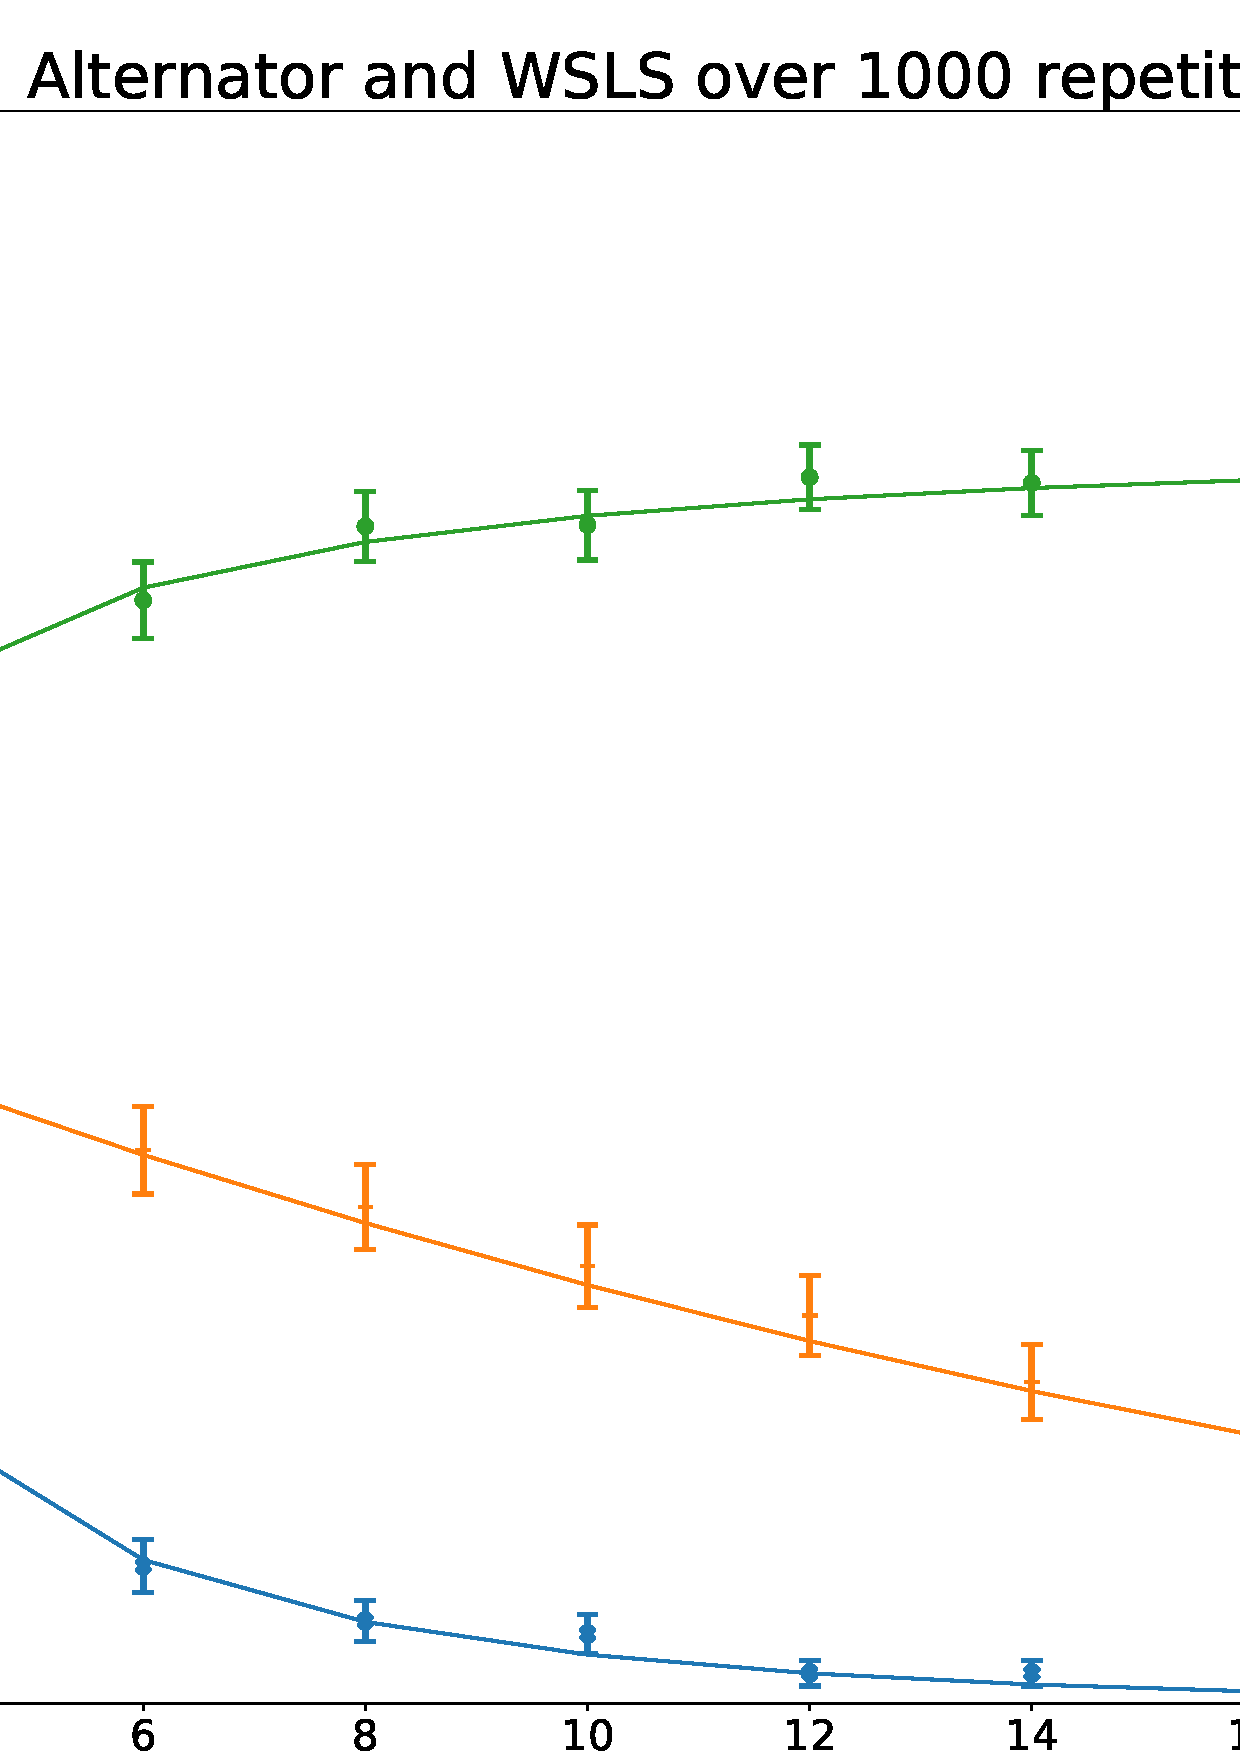
\includegraphics[width=.95\columnwidth]{./Alternator_v_WSLS.pdf}
    \caption{Comparison of theoretic and actual Moran Process fixation
             probabilities for \textit{deterministic} strategies: Alternator and
         Cooperator. 5\% confidence intervals calculated using an asymptotic
     normal approximation.
The top most line on all figures (in red and using a circle) corresponds to
\(x_{N-1}\), the middle line (in green and using a cross) corresponds to
\(x_{N/2}\) and the bottom line (in blue and using an x) corresponds to
\(x_{1}\).}
    \label{fig:comparison_deterministic}
\end{figure}

\begin{table}[!hbtp]
    \centering

        \begin{tabular}{rrrr}
        \toprule
          N &  $p_1$ $p$ Value &  $p_{N / 2}$ $p$ Value &  $p_{N - 1}$ $p$ Value \\
        \midrule
          2 &          0.89942 &                0.89942 &                0.89942 \\
          4 &          0.16344 &                0.74768 &                0.85877 \\
          6 &          0.65406 &                0.84051 &                0.51992 \\
          8 &          0.92617 &                0.45748 &                0.38604 \\
         10 &          0.03505 &                0.37115 &                0.60635 \\
         12 &          0.96697 &                0.20790 &                0.18124 \\
         14 &          0.08126 &                0.63771 &                0.76246 \\
         16 &          0.59434 &                0.07697 &                0.42520 \\
         18 &          0.05339 &                0.47126 &                0.94814 \\
         20 &          0.30805 &                0.79795 &                0.82381 \\
        \bottomrule
        \end{tabular}

    \caption{\(p\) values resulting from a $t$ test comparing the theoretic
        value with the simulated value of the Moran Process fixation
        probabilities for \textit{deterministic} strategies: Alternator and
    Cooperator.}
    \label{tab:comparison_deterministic}
\end{table}

\begin{figure}[!hbtp]
    \centering
    \includegraphics[width=.95\columnwidth]{./Calculator_v_Arrogant_QLearner.pdf}
    \caption{Comparison of theoretic and actual Moran Process
             fixation probabilities for \textit{stochastic} strategies:
             Calculator and Arrogant Q Learner. 5\% confidence intervals calculated using an asymptotic
     normal approximation.
The top most line on all figures (in red and using a circle) corresponds to
\(x_{N-1}\), the middle line (in green and using a cross) corresponds to
\(x_{N/2}\) and the bottom line (in blue and using an x) corresponds to
\(x_{1}\).}
    \label{fig:comparison_stochastic}
\end{figure}

\begin{table}[!hbtp]
    \centering
        \begin{tabular}{rrrr}
        \toprule
          N &  $p_1$ $p$ Value &  $p_{N / 2}$ $p$ Value &  $p_{N - 1}$ $p$ Value \\
        \midrule
          2 &          0.05372 &                0.05372 &                0.05372 \\
          4 &          0.34188 &                0.00940 &                0.00005 \\
          6 &          0.16510 &                0.00000 &                0.00000 \\
          8 &          0.03451 &                0.00000 &                0.00000 \\
         10 &          0.00543 &                0.00000 &                0.00000 \\
         12 &          0.19646 &                0.00000 &                0.00000 \\
         14 &          0.00814 &                0.00000 &                0.00000 \\
         16 &          0.01038 &                0.00000 &                0.00000 \\
         18 &          0.39556 &                0.00000 &                0.00000 \\
         20 &          0.00030 &                0.00000 &                0.00000 \\
        \bottomrule
        \end{tabular}
    \caption{\(p-\text{values}\) resulting from a \(t-\text{ test}\) comparing the theoretic
        value with the simulated value of the Moran Process fixation
        probabilities for \textit{stochastic} strategies: Calculator and
    Arrogant Q Learner.}
    \label{tab:comparison_stochastic}
\end{table}

\subsection*{Empirical results}

This section outlines the data analysis carried out, all data for this study is
available at~\cite{data}.

\begin{itemize}
    \item First the specific case of
        \(N=2\) is considered.
    \item The effect of
        population size on the ability of a strategy to invade another
        population is investigated. This will highlight how complex strategies with long
        memories outperform simpler strategies.
    \item Then a similar investigation of the
        ability to defend against an invasion is given.
    \item Finally the relationship
        between performance for differing population sizes as well as
        taking a close look at zero determinant strategies \cite{Press2012} is
        analysed.
\end{itemize}

\subsubsection*{The special case of \(N=2\)}

When $N=2$ the fixation probabilities of the Moran process are effectively measures
of the distribution of  relative
mean payoffs over all possible matches between two players. The strategy
that scores higher than the other more often will fixate more often. For \(N=2\)
the two cases of \(x_1\) and \(x_{N-1}\) coincide, but will be
considered separately for larger \(N\) in the following sections.
The top 16 (10\%) strategies are
shown in

Table~\ref{tbl:summary_top_2} and figures showing the performance of all
strategies are available in the appendix.
The top five ranking strategies are:

\begin{enumerate}
    \item The top strategy is the Collective Strategy (CS) which has a simple
        handshake mechanism described above.
    \item Defector: it always defects. Since it has no interactions with other
        defectors (recall that \(N=2\)), its aggressiveness is rewarded.
    \item Aggravater, which plays like Grudger (responding to any
        defections with unconditional defections throughout) however starts by
        playing 3 defections.
    \item Predator, a finite state machine described in \cite{Ashlock2006}.
    \item Handshake, a slightly less aggressive version of the Collective
        Strategy \cite{Robson1990}. As long as the initial sequence is played
        then it cooperates. Thus it will do well in a population consisting of
        many members of itself just as the Collective Strategy does. The
        difference is that CS will defect after the handshake if the opponent
        defects while Handshake will not.
\end{enumerate}

It is also noted that TF1, TF2 and TF3 all perform well. This is also the \(N\)
for which a zero determinant strategy does appear in the top 10\% ranking
strategies: ZD-extort-4. The performance of zero determinant strategies will be
examined more closely.

\begin{table}[!hbtp]
    \tiny
    \centering
    \scalebox{0.95}{
        \begin{tabular}{llrrrrrrr}
        \toprule
        {} &                  Player &    Min &   5th \% &    Mean &  Median &  95th \% &    Max &     Std \\
        \midrule
        1  &                      CS &  0.497 &  0.5020 &  0.6651 &   0.572 &  0.9908 &  0.993 &  0.1800 \\
        2  &                Defector &  0.502 &  0.5020 &  0.6496 &   0.518 &  1.0000 &  1.000 &  0.1767 \\
        3  &              Aggravater &  0.502 &  0.5020 &  0.6328 &   0.518 &  0.9790 &  0.999 &  0.1660 \\
        4  &                Predator &  0.319 &  0.4980 &  0.6301 &   0.551 &  0.9870 &  0.993 &  0.1676 \\
        5  &               Handshake &  0.006 &  0.4503 &  0.6240 &   0.524 &  0.9908 &  0.993 &  0.1889 \\
        6  &                Prober 4 &  0.431 &  0.4620 &  0.6183 &   0.534 &  0.9579 &  0.958 &  0.1656 \\
        7  &                     \textbf{TF1} &  0.430 &  0.4980 &  0.6171 &   0.544 &  0.9240 &  0.981 &  0.1345 \\
        8  &                Prober 3 &  0.497 &  0.5011 &  0.6044 &   0.505 &  0.9930 &  0.993 &  0.1683 \\
        9  &                     \textbf{TF2} &  0.324 &  0.5020 &  0.6026 &   0.565 &  0.8362 &  0.887 &  0.1092 \\
        10 &                 Grudger &  0.497 &  0.5020 &  0.5996 &   0.502 &  0.9840 &  0.989 &  0.1695 \\
        11 &       Better and Better &  0.388 &  0.3951 &  0.5980 &   0.514 &  0.9300 &  0.934 &  0.1865 \\
        12 &                    MEM2 &  0.497 &  0.5001 &  0.5942 &   0.502 &  0.9840 &  0.987 &  0.1656 \\
        13 &  Meta Hunter Aggressive &  0.247 &  0.2943 &  0.5933 &   0.517 &  0.9498 &  0.981 &  0.2013 \\
        14 &                     \textbf{TF3} &  0.344 &  0.4971 &  0.5927 &   0.502 &  0.9790 &  0.982 &  0.1617 \\
        15 &            Fool Me Once &  0.494 &  0.4980 &  0.5892 &   0.502 &  0.9790 &  0.982 &  0.1625 \\
        16 &             ZD-Extort-4 &  0.497 &  0.5020 &  0.5867 &   0.584 &  0.6900 &  0.695 &  0.0724 \\
        \bottomrule
        \end{tabular}
    }
    \caption{Top strategies for \(N=2\) (neutral fixation is \(p=0.5\))}
    \label{tbl:summary_top_2}
\end{table}

As will be demonstrated the results for
\(N=2\) differ from those of larger $N$. Hence these results do not concur with
the literature which suggests that zero determinant strategies should be
effective for larger population sizes, but these analyses consider stationary
behaviour, while this work runs for a fixed number of rounds \cite{stewart2013extortion}.
The stationarity assumption allows for a deterministic payoff matrix
leading to the conclusions about zero determinant strategies in the space
of memory-one strategies that do not generalize to this context.

% In the next sections close attention to
% strategies who are strong invaders/resistors is given.

\subsubsection*{Strong Invaders}

In this section the focus is on the ability of a mutant strategy to invade: the
probability of one individual of a given type successfully fixating in a
population of \(N - 1\) other individuals, denoted by \(x_1\). The ranks of each
strategy for all considered values of \(N\) according to mean \(x_1\) are shown
in Fig~\ref{fig:ranks_v_size_invade}.

\begin{figure}[!hbtp]
    \centering
    \includegraphics[width=\columnwidth]{./average_rank_vs_population_size_invade.pdf}
    \caption{\textbf{Invasion}: Ranks of all strategies according to \(x_1\) for different population sizes.}
    \label{fig:ranks_v_size_invade}
\end{figure}

The top 16 strategies are given in Table~\ref{tbl:top_invade}. A variety of
figures showing the performance of all strategies is available in the
appendix.

\begin{table}[!hbtp]
    \centering
    \tiny
    \begin{subfigure}[t]{\columnwidth}
        \centering
            \begin{tabular}{llrrrrrrr}
            \toprule
            {} &                   Player &    Min &   5th \% &    Mean &  Median &  95th \% &    Max &     Std \\
            \midrule
            1  &                       CS &  0.261 &  0.2620 &  0.4478 &   0.403 &  0.8105 &  0.908 &  0.1998 \\
            2  &                  Grudger &  0.259 &  0.2641 &  0.4313 &   0.338 &  0.8097 &  0.908 &  0.1699 \\
            3  &                     MEM2 &  0.258 &  0.2875 &  0.4278 &   0.338 &  0.7977 &  0.907 &  0.1636 \\
            4  &                      \textbf{TF3} &  0.248 &  0.2610 &  0.4267 &   0.338 &  0.7904 &  0.904 &  0.1624 \\
            5  &                 Prober 4 &  0.221 &  0.2400 &  0.4242 &   0.365 &  0.7723 &  0.891 &  0.1755 \\
            6  &             Fool Me Once &  0.257 &  0.2645 &  0.4242 &   0.338 &  0.7938 &  0.904 &  0.1620 \\
            7  &                    Davis &  0.234 &  0.2581 &  0.4218 &   0.338 &  0.7759 &  0.891 &  0.1590 \\
            8  &                 Predator &  0.173 &  0.2590 &  0.4210 &   0.374 &  0.7845 &  0.907 &  0.1824 \\
            9  &            Evolved ANN 5 &  0.255 &  0.3163 &  0.4163 &   0.338 &  0.7872 &  0.879 &  0.1530 \\
            10 &              Evolved ANN &  0.253 &  0.2789 &  0.4163 &   0.338 &  0.7938 &  0.906 &  0.1572 \\
            11 &           Evolved FSM 16 &  0.041 &  0.1391 &  0.4154 &   0.338 &  0.7977 &  0.907 &  0.1830 \\
            12 &              Meta Hunter &  0.123 &  0.2541 &  0.4140 &   0.338 &  0.7807 &  0.892 &  0.1614 \\
            13 &                      \textbf{TF1} &  0.257 &  0.2580 &  0.4139 &   0.398 &  0.7411 &  0.900 &  0.1529 \\
            14 &        PSO Gambler 2\_2\_2 &  0.073 &  0.2643 &  0.4134 &   0.338 &  0.7938 &  0.904 &  0.1727 \\
            15 &     EvolvedLookerUp1\_1\_1 &  0.258 &  0.3004 &  0.4113 &   0.338 &  0.7515 &  0.830 &  0.1369 \\
            16 &  Evolved FSM 16 Noise 05 &  0.247 &  0.3238 &  0.4107 &   0.338 &  0.7977 &  0.906 &  0.1540 \\
            \bottomrule
            \end{tabular}
        \caption{\(N=3\)}
    \end{subfigure}%

    \begin{subfigure}[t]{\columnwidth}
        \centering
            \begin{tabular}{llrrrrrrr}
            \toprule
            {} &                   Player &    Min &   5th \% &    Mean &  Median &  95th \% &    Max &     Std \\
            \midrule
            1  &           Evolved FSM 16 &  0.001 &  0.0313 &  0.2523 &   0.142 &  0.6389 &  0.826 &  0.1931 \\
            2  &        PSO Gambler 2\_2\_2 &  0.004 &  0.0588 &  0.2467 &   0.142 &  0.6096 &  0.826 &  0.1809 \\
            3  &             Fool Me Once &  0.044 &  0.0470 &  0.2459 &   0.142 &  0.6105 &  0.826 &  0.1792 \\
            4  &            Evolved ANN 5 &  0.044 &  0.1092 &  0.2450 &   0.142 &  0.6010 &  0.812 &  0.1722 \\
            5  &              Evolved ANN &  0.042 &  0.0615 &  0.2449 &   0.142 &  0.6104 &  0.826 &  0.1785 \\
            6  &     EvolvedLookerUp2\_2\_2 &  0.000 &  0.0618 &  0.2443 &   0.142 &  0.6380 &  0.824 &  0.1822 \\
            7  &                  Grudger &  0.044 &  0.0451 &  0.2442 &   0.142 &  0.6420 &  0.826 &  0.1830 \\
            8  &                     MEM2 &  0.044 &  0.0583 &  0.2436 &   0.142 &  0.6143 &  0.826 &  0.1760 \\
            9  &                      \textbf{TF3} &  0.044 &  0.0450 &  0.2430 &   0.142 &  0.6344 &  0.826 &  0.1779 \\
            10 &        PSO Gambler 1\_1\_1 &  0.021 &  0.1033 &  0.2404 &   0.142 &  0.6381 &  0.824 &  0.1710 \\
            11 &                       CS &  0.045 &  0.0450 &  0.2395 &   0.148 &  0.6385 &  0.826 &  0.2169 \\
            12 &  Evolved FSM 16 Noise 05 &  0.044 &  0.1298 &  0.2394 &   0.142 &  0.6143 &  0.826 &  0.1732 \\
            13 &            Evolved HMM 5 &  0.010 &  0.0611 &  0.2390 &   0.142 &  0.6115 &  0.826 &  0.1785 \\
            14 &              Meta Hunter &  0.015 &  0.0465 &  0.2385 &   0.142 &  0.5993 &  0.820 &  0.1751 \\
            15 &                    Davis &  0.036 &  0.0465 &  0.2379 &   0.142 &  0.5953 &  0.820 &  0.1732 \\
            16 &         PSO Gambler Mem1 &  0.018 &  0.1105 &  0.2348 &   0.142 &  0.6370 &  0.825 &  0.1671 \\
            \bottomrule
            \end{tabular}
        \caption{\(N=7\)}
    \end{subfigure}

    \begin{subfigure}[t]{\columnwidth}
        \centering
            \begin{tabular}{llrrrrrrr}
            \toprule
            {} &                   Player &    Min &   5th \% &    Mean &  Median &  95th \% &    Max &     Std \\
            \midrule
            1  &           Evolved FSM 16 &  0.000 &  0.0054 &  0.2096 &   0.079 &  0.7241 &  0.842 &  0.2172 \\
            2  &        PSO Gambler 2\_2\_2 &  0.000 &  0.0113 &  0.2042 &   0.079 &  0.5940 &  0.842 &  0.2045 \\
            3  &     EvolvedLookerUp2\_2\_2 &  0.000 &  0.0270 &  0.2014 &   0.079 &  0.6608 &  0.840 &  0.2097 \\
            4  &              Evolved ANN &  0.002 &  0.0164 &  0.2014 &   0.079 &  0.5939 &  0.842 &  0.2074 \\
            5  &            Evolved ANN 5 &  0.002 &  0.0505 &  0.2004 &   0.079 &  0.5940 &  0.834 &  0.2009 \\
            6  &            Evolved HMM 5 &  0.000 &  0.0321 &  0.1972 &   0.079 &  0.5940 &  0.842 &  0.2034 \\
            7  &        PSO Gambler 1\_1\_1 &  0.001 &  0.0455 &  0.1955 &   0.079 &  0.6150 &  0.841 &  0.1931 \\
            8  &             Fool Me Once &  0.002 &  0.0058 &  0.1955 &   0.079 &  0.5940 &  0.842 &  0.2032 \\
            9  &  Evolved FSM 16 Noise 05 &  0.003 &  0.0607 &  0.1943 &   0.079 &  0.5930 &  0.842 &  0.2005 \\
            10 &         PSO Gambler Mem1 &  0.000 &  0.0517 &  0.1920 &   0.079 &  0.6118 &  0.841 &  0.1907 \\
            11 &            Evolved FSM 4 &  0.000 &  0.0000 &  0.1918 &   0.079 &  0.5930 &  0.842 &  0.2049 \\
            12 &              Meta Hunter &  0.000 &  0.0049 &  0.1869 &   0.079 &  0.5883 &  0.840 &  0.1882 \\
            13 &   Evolved ANN 5 Noise 05 &  0.001 &  0.0303 &  0.1858 &   0.079 &  0.5930 &  0.840 &  0.1968 \\
            14 &                Omega TFT &  0.003 &  0.0704 &  0.1849 &   0.079 &  0.5939 &  0.840 &  0.1927 \\
            15 &                Fortress4 &  0.000 &  0.0000 &  0.1848 &   0.066 &  0.5919 &  0.840 &  0.2211 \\
            16 &                      \textbf{TF3} &  0.002 &  0.0041 &  0.1846 &   0.079 &  0.6190 &  0.842 &  0.1890 \\
            \bottomrule
            \end{tabular}
        \caption{\(N=14\)}
    \end{subfigure}
    \caption{Top invaders for \(N\in\{3, 7, 14\}\)}
    \label{tbl:top_invade}
\end{table}

It can be seen that apart from CS, none of the strategies for \(N=2\)
of Table~\ref{tbl:summary_top_2} perform well for \(N\in\{3, 7, 14\}\). The new
top performing strategies are:

\begin{itemize}
    \item Grudger (which only performs well for \(N=3\)), starts by cooperating
        but will defect if at any point the opponent has defected.
    \item MEM2, an infinite memory strategy that switches between TFT, TF2T, and
        Defector \cite{Li2014}.
    \item TF3, the finite state machine trained specifically for Moran processes
        described.
    \item Prober 4, a strategy which starts with a specific 20 move sequence of
        cooperations and defections \cite{Prison1998}. This initial sequence serves
        as approximate handshake.
    \item  PSO Gambler and Evolved Lookerup 2 2 2: strategies that make use
        of a lookup table mapping the first 2 moves of the opponent as well as
        the last 2 moves of both players to an action.  PSO gambler is a
        stochastic version of  Lookerup which maps those states to probabilities
       of cooperating. Lookerup was described in \cite{Knight2016}.
    \item The Evolved ANN strategies are neural networks that map a number of
	    attributes (first move, number of cooperations, last move, etc.) to
	    an action. Both of these have been trained using an evolutionary
	    algorithm.
    \item Evolved FSM 16 is a 16 state finite state machine trained to
        perform well in tournaments.
\end{itemize}

Only one of the above strategies is stochastic although close inspection of the
source code of PSO Gambler shows that it makes stochastic decisions rarely, and
is functionally very similar to its deterministic cousin Evolved Looker Up.
PSO Gambler Mem1 is a stochastic memory one strategy that has been trained to
maximise its utility and does perform well.
Apart from TF3, the finite state machines trained specifically for
Moran processes do not appear in the top 5, while strategies trained for
tournaments do. This is due to the nature of invasion: most of the opponents
will initially be different strategies. The next section will consider the
converse situation.

\subsubsection*{Strong Resistors}

In addition to identifying good invaders, strategies resistant to invasion by
other strategies are identified by examining the distribution of $x_{N-1}$ for
each strategy. The ranks of each strategy for all considered values of \(N\)
according to mean \(x_{N-1}\) are shown in Fig~\ref{fig:ranks_v_size_resist}.

\begin{figure}[!hbtp]
    \centering
    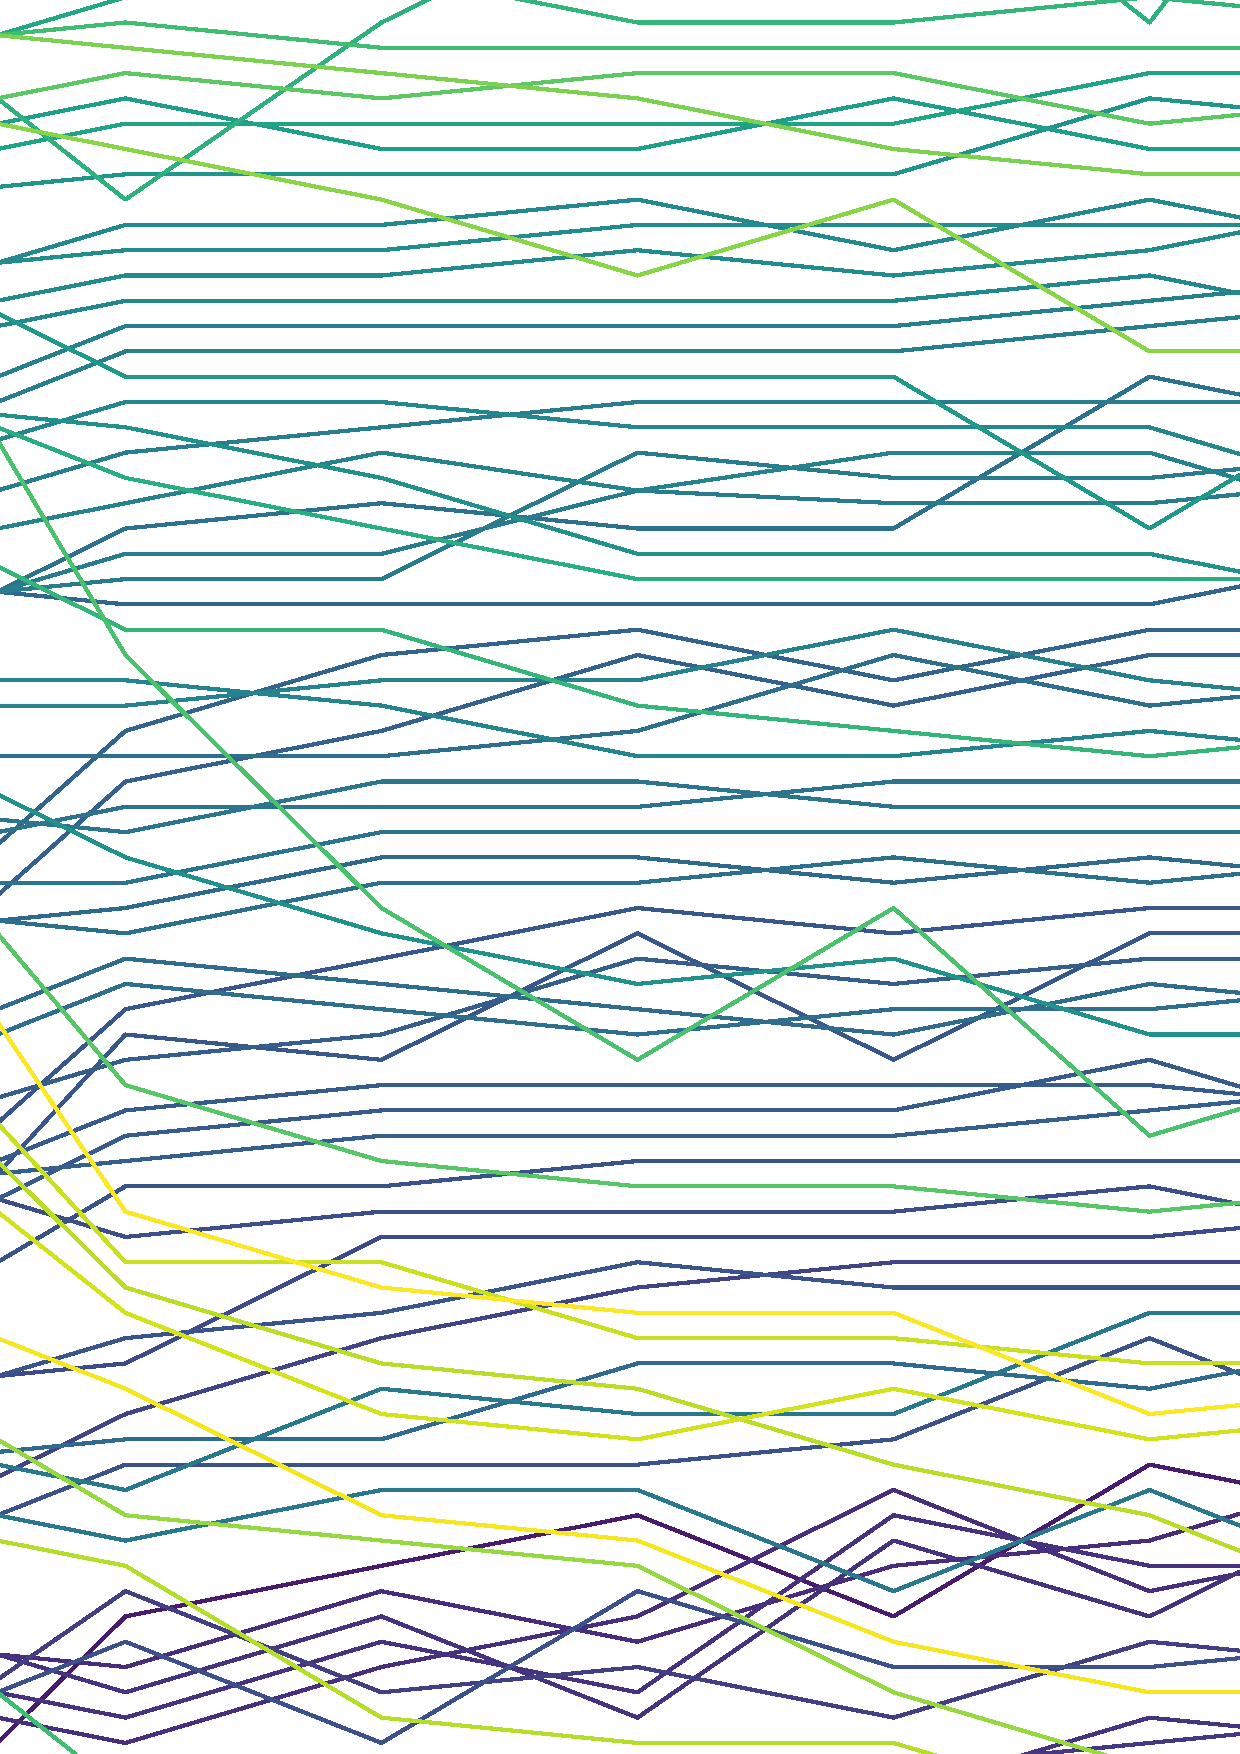
\includegraphics[width=\columnwidth]{./average_rank_vs_population_size_resist.pdf}
    \caption{\textbf{Resistance}: Ranks of all strategies according to \(x_{N-1}\) for different
    population sizes.}
    \label{fig:ranks_v_size_resist}
\end{figure}


Table~\ref{tbl:top_resist} shows the top strategies when ranked
according to \(x_{N-1}\) for \(N\in\{3, 7, 14\}\) and figures showing results
for all strategies are available in the supplementary materials.
Once again none of the short memory strategies previously discussed perform well for high \(N\).

\begin{table}[!hbtp]
    \tiny
    \centering
    \begin{subfigure}[t]{\columnwidth}
        \centering
            \begin{tabular}{llrrrrrrr}
            \toprule
            {} &                Player &    Min &   5th \% &    Mean &  Median &  95th \% &    Max &     Std \\
            \midrule
            1  &                    CS &  0.662 &  0.7410 &  0.8359 &   0.796 &  0.9980 &  1.000 &  0.0981 \\
            2  &              Predator &  0.530 &  0.7363 &  0.8121 &   0.789 &  0.9980 &  1.000 &  0.0983 \\
            3  &                   \textbf{TF1} &  0.648 &  0.7330 &  0.8087 &   0.791 &  0.9745 &  0.999 &  0.0775 \\
            4  &             Handshake &  0.225 &  0.6322 &  0.8014 &   0.779 &  0.9980 &  1.000 &  0.1293 \\
            5  &                   \textbf{TF2} &  0.572 &  0.7363 &  0.7957 &   0.790 &  0.9330 &  0.961 &  0.0672 \\
            6  &              Prober 4 &  0.646 &  0.6610 &  0.7905 &   0.750 &  0.9890 &  0.996 &  0.1070 \\
            7  &               Grudger &  0.662 &  0.6620 &  0.7612 &   0.662 &  0.9980 &  1.000 &  0.1224 \\
            8  &           Hard Prober &  0.661 &  0.6620 &  0.7582 &   0.732 &  0.9980 &  0.999 &  0.1079 \\
            9  &                   \textbf{TF3} &  0.594 &  0.6620 &  0.7570 &   0.662 &  0.9969 &  0.999 &  0.1197 \\
            10 &                  MEM2 &  0.662 &  0.6620 &  0.7554 &   0.662 &  0.9980 &  1.000 &  0.1210 \\
            11 &                 Davis &  0.662 &  0.6620 &  0.7536 &   0.662 &  0.9848 &  0.996 &  0.1164 \\
            12 &              Winner21 &  0.662 &  0.6630 &  0.7529 &   0.742 &  0.9218 &  0.948 &  0.0741 \\
            13 &          Fool Me Once &  0.661 &  0.6620 &  0.7489 &   0.662 &  0.9970 &  0.999 &  0.1191 \\
            14 &             Fortress4 &  0.552 &  0.5520 &  0.7467 &   0.707 &  1.0000 &  1.000 &  0.1676 \\
            15 &           Retaliate 3 &  0.662 &  0.6620 &  0.7448 &   0.662 &  0.9538 &  0.986 &  0.1032 \\
            16 &  EvolvedLookerUp1\_1\_1 &  0.662 &  0.6620 &  0.7422 &   0.662 &  0.9792 &  0.998 &  0.1062 \\
            \bottomrule
            \end{tabular}
        \caption{\(N=3\)}
    \end{subfigure}%

    \begin{subfigure}[t]{\columnwidth}
        \centering
            \begin{tabular}{llrrrrrrr}
            \toprule
            {} &       Player &    Min &   5th \% &    Mean &  Median &  95th \% &    Max &     Std \\
            \midrule
            1  &           CS &  0.858 &  0.9560 &  0.9765 &   0.981 &   1.000 &  1.000 &  0.0203 \\
            2  &          \textbf{TF1} &  0.866 &  0.9521 &  0.9714 &   0.979 &   1.000 &  1.000 &  0.0207 \\
            3  &          \textbf{TF2} &  0.840 &  0.9423 &  0.9677 &   0.976 &   0.998 &  1.000 &  0.0239 \\
            4  &     Predator &  0.741 &  0.9478 &  0.9677 &   0.970 &   1.000 &  1.000 &  0.0367 \\
            5  &    Handshake &  0.448 &  0.8261 &  0.9547 &   0.970 &   1.000 &  1.000 &  0.0848 \\
            6  &     Prober 4 &  0.837 &  0.8500 &  0.9540 &   0.955 &   1.000 &  1.000 &  0.0416 \\
            7  &     Winner21 &  0.858 &  0.8600 &  0.9392 &   0.956 &   0.996 &  0.999 &  0.0486 \\
            8  &  Hard Prober &  0.856 &  0.8560 &  0.9331 &   0.953 &   1.000 &  1.000 &  0.0521 \\
            9  &    Fortress4 &  0.829 &  0.8290 &  0.9255 &   0.925 &   1.000 &  1.000 &  0.0653 \\
            10 &      Grudger &  0.858 &  0.8580 &  0.9198 &   0.858 &   1.000 &  1.000 &  0.0642 \\
            11 &          \textbf{TF3} &  0.858 &  0.8580 &  0.9189 &   0.858 &   1.000 &  1.000 &  0.0638 \\
            12 &        Davis &  0.858 &  0.8580 &  0.9186 &   0.858 &   1.000 &  1.000 &  0.0633 \\
            13 &       Ripoff &  0.856 &  0.8560 &  0.9183 &   0.922 &   0.986 &  0.988 &  0.0484 \\
            14 &       Tester &  0.856 &  0.8560 &  0.9176 &   0.921 &   0.986 &  0.988 &  0.0486 \\
            15 &         MEM2 &  0.858 &  0.8580 &  0.9165 &   0.858 &   1.000 &  1.000 &  0.0636 \\
            16 &  Retaliate 3 &  0.858 &  0.8580 &  0.9161 &   0.858 &   0.999 &  1.000 &  0.0619 \\
            \bottomrule
            \end{tabular}
        \caption{\(N=7\)}
    \end{subfigure}

    \begin{subfigure}[t]{\columnwidth}
        \centering
        \begin{tabular}{llrrrrrrr}
        \toprule
        {} &       Player &    Min &   5th \% &    Mean &  Median &  95th \% &  Max &     Std \\
        \midrule
        1  &           CS &  0.921 &  0.9970 &  0.9984 &   1.000 &     1.0 &  1.0 &  0.0062 \\
        2  &          \textbf{TF1} &  0.938 &  0.9950 &  0.9973 &   0.999 &     1.0 &  1.0 &  0.0069 \\
        3  &          \textbf{TF2} &  0.925 &  0.9820 &  0.9949 &   0.996 &     1.0 &  1.0 &  0.0104 \\
        4  &     Predator &  0.836 &  0.9912 &  0.9941 &   0.999 &     1.0 &  1.0 &  0.0212 \\
        5  &     Prober 4 &  0.895 &  0.9110 &  0.9863 &   0.996 &     1.0 &  1.0 &  0.0250 \\
        6  &    Handshake &  0.514 &  0.9131 &  0.9812 &   0.999 &     1.0 &  1.0 &  0.0743 \\
        7  &     Winner21 &  0.921 &  0.9210 &  0.9778 &   0.996 &     1.0 &  1.0 &  0.0310 \\
        8  &  Hard Prober &  0.916 &  0.9160 &  0.9731 &   0.995 &     1.0 &  1.0 &  0.0327 \\
        9  &    Fortress4 &  0.929 &  0.9290 &  0.9726 &   0.981 &     1.0 &  1.0 &  0.0287 \\
        10 &       Ripoff &  0.919 &  0.9190 &  0.9669 &   0.978 &     1.0 &  1.0 &  0.0318 \\
        11 &       Tester &  0.919 &  0.9190 &  0.9662 &   0.977 &     1.0 &  1.0 &  0.0320 \\
        12 &      Grudger &  0.921 &  0.9210 &  0.9592 &   0.921 &     1.0 &  1.0 &  0.0390 \\
        13 &          \textbf{TF3} &  0.921 &  0.9210 &  0.9589 &   0.921 &     1.0 &  1.0 &  0.0388 \\
        14 &        Davis &  0.921 &  0.9210 &  0.9588 &   0.921 &     1.0 &  1.0 &  0.0387 \\
        15 &  Retaliate 3 &  0.921 &  0.9210 &  0.9580 &   0.921 &     1.0 &  1.0 &  0.0383 \\
        16 &    Retaliate &  0.921 &  0.9210 &  0.9576 &   0.921 &     1.0 &  1.0 &  0.0382 \\
        \bottomrule
        \end{tabular}
        \caption{\(N=14\)}
    \end{subfigure}
    \caption{Top resistors for \(N\in\{3, 7, 14\}\)}
    \label{tbl:top_resist}
\end{table}

Interestingly none of these strategies are stochastic: this is explained by the
value of not provoking typically cooperative opponent strategies with
speculative defections. This includes opponents using the same strategy.  Acting
stochastically increases the chance of reducing the score of individuals of the
same type in a Moran process.  However it is possible to design a strategy with
a stochastic or error-correcting handshake that is an excellent resistor even in
noisy environments \cite{Lee2015}.

There are only two new strategies that appear in the top ranks for
\(x_{N-1}\): TF1 and TF2. These two strategies are with CS the strongest
resistors. They all have handshakes, and whilst the handshakes of CS and
Handshake (which ranks highly for the smaller values of \(N\)) were
programmed, the handshakes of TF1 and TF2 evolved through an evolutionary
process without any priming.

As described previously the strategies trained with
the payoff maximizing objective are among the best invaders in the library
however they are not as resistant to invasion as the strategies trained using a
Moran objective function. These strategies include trained finite state machine
strategies, but they do not appear to have handshaking mechanisms. Therefore it
is reasonable to conclude that the objective function is the cause of the
emergence of handshaking mechanisms. More specifically, TF1 and TF2 evolved
handshakes for high invasion resistance. TF3 is a better total payoff maximizer
which makes it a better invader along with the strategies
trained to maximize total payoff since successful fitness proportionate selection
is necessary for invasion. Training with an objective with initial population
mix other than $(N/2, N/2)$ may favor invasion or resistance.

The payoff maximizing strategies typically will not defect before the opponent's
first defection, possibly because the training strategy collection contains some
strategies such as Grudger and Fool Me Once that retaliate harshly by defecting
for the remainder of the match if the opponent has more than a small number of
cumulative defections. Paradoxically for handshaking strategies
it is advantageous to defect (as a signal)
in order to achieve mutual cooperation with opponents using the same strategy
but not with other opponents. Nevertheless an evolutionary process is able to
tunnel through the costs and risks associated with early defections to find more
optimal solutions, so it is not surprising in hindsight that handshaking
strategies emerge from the evolutionary training process.

A handshake requires at least one defection and there is
selective pressure to defect as few times as possible to achieve the
self-recognition mechanism. It is also unwise to defect on the first move as
some strategies additionally retaliate in response to first round defections. So the
handshakes used by TF1, TF2, and CS are in some sense optimal.

It is evident through
the work presented that performance of strategies not only depends
on the initial population distribution but also that there seems to be a
difference depending on whether or not \(N>2\). This will be explored further in
the next section, looking not only at \(x_1\) and \(x_{N-1}\) but also
considering
\(x_{N/2}\).

\subsubsection*{The effect of population size}

Fig~\ref{fig:ranks_v_size_coexist} complements
Figs~\ref{fig:ranks_v_size_invade} and~\ref{fig:ranks_v_size_resist} showing the
ranks of each strategy for all considered even values of \(N\) according to mean
\(x_{N/2}\).

\begin{figure}[!hbtp]
    \centering
    \includegraphics[width=\columnwidth]{./average_rank_vs_population_size_coexist.pdf}
    \caption{Fixation ranks of all strategies according to \(x_{N/2}\) for different
    population sizes.}
    \label{fig:ranks_v_size_coexist}
\end{figure}

Tables~\ref{tbl:ranks_v_size_invade},~\ref{tbl:ranks_v_size_resist}
and~\ref{tbl:ranks_v_size_coexist} show the ranks for a selection of
strategies:

\begin{itemize}
    \item The strategies that ranked highly for \(N=2\);
    \item The strategies that ranked highly for \(N=14\);
    \item The zero determinant strategies.
\end{itemize}

The results for \(x_{N/2}\) show similarities to the results for \(x_{N-1}\) and
in particular TF1, TF2 and TF3 ranked one, three and eight. This is to be
expected since, as described previously these strategies
were trained in an initial population of \((N/2, N/2)\) individuals.

For all starting populations
\(i\in\{1, N/2, N-1\}\) the ranks of strategies are relatively stable across the
different values of \(N>2\) however for \(N=2\) there is a distinct difference.
This highlights that there is little that can be inferred about the evolutionary
performance of a strategy in a large population from its performance in a small
population. This is confirmed by the performance of the zero determinant strategies: while
some do rank relatively highly for \(N=2\) (ZD-Extort-4 has rank 16) this rank
does not translate to larger populations.

\begin{table}[!hbtp]
    \centering
    \scriptsize
    \scalebox{0.7}{
        \begin{tabular}{lrrrrrrrrrrrrr}
        \toprule
                         Size &      2 &      3 &      4 &      5 &      6 &      7 &      8 &      9 &     10 &     11 &     12 &     13 &     14 \\
        \midrule
                           CS &    1 &    1 &    2 &   11 &    9 &   11 &   13 &   21 &   16 &   22 &   17 &   25 &   23 \\
                     Defector &    2 &   43 &   80 &   91 &   89 &   87 &   87 &  103 &   97 &  105 &   94 &  103 &  101 \\
                   Aggravater &    3 &   50 &   89 &   99 &  102 &  103 &  108 &  113 &  114 &  115 &  115 &  116 &  117 \\
                     Predator &    4 &    8 &   24 &   35 &   28 &   33 &   31 &   43 &   36 &   43 &   34 &   45 &   35 \\
                    Handshake &    5 &   17 &   40 &   46 &   43 &   46 &   46 &   49 &   48 &   49 &   47 &   50 &   49 \\
        \midrule
               Evolved FSM 16 &   31 &   11 &    6 &    2 &    1 &    1 &    1 &    1 &    1 &    1 &    1 &    1 &    1 \\
            PSO Gambler 2\_2\_2 &   29 &   14 &   10 &    6 &    4 &    2 &    2 &    2 &    2 &    2 &    2 &    2 &    2 \\
         EvolvedLookerUp2\_2\_2 &   33 &   18 &   11 &    9 &   10 &    6 &    6 &    5 &    3 &    5 &    3 &    3 &    3 \\
                  Evolved ANN &   20 &   10 &    8 &    7 &    8 &    5 &    3 &    3 &    4 &    3 &    4 &    4 &    4 \\
                Evolved ANN 5 &   21 &    9 &    7 &    8 &    7 &    4 &    5 &    4 &    5 &    4 &    5 &    5 &    5 \\
        \midrule
                          \textbf{TF1} &    7 &   13 &   33 &   38 &   30 &   39 &   42 &   46 &   42 &   46 &   41 &   46 &   46 \\
                          \textbf{TF2} &    9 &   19 &   29 &   33 &   19 &   28 &   29 &   38 &   27 &   34 &   26 &   32 &   30 \\
                          \textbf{TF3} &   14 &    4 &    5 &    5 &    6 &    9 &   11 &   11 &   12 &   14 &   13 &   13 &   16 \\
        \midrule
                  ZD-Extort-4 &   16 &   81 &  107 &  120 &  135 &  136 &  142 &  140 &  142 &  142 &  144 &  144 &  145 \\
               ZD-Extort-2 v2 &   41 &  105 &  126 &  140 &  152 &  152 &  153 &  152 &  153 &  153 &  153 &  152 &  153 \\
                  ZD-Extort-2 &   43 &  107 &  125 &  139 &  151 &  151 &  152 &  153 &  152 &  152 &  152 &  153 &  152 \\
                     ZD-SET-2 &  100 &  111 &  117 &  117 &  122 &  127 &  131 &  128 &  131 &  131 &  130 &  132 &  131 \\
                    ZD-GTFT-2 &  112 &   92 &   82 &   80 &   81 &   82 &   84 &   72 &   81 &   71 &   78 &   72 &   70 \\
                     ZD-GEN-2 &  113 &   96 &   87 &   83 &   85 &   88 &   90 &   82 &   87 &   82 &   86 &   83 &   91 \\
        \bottomrule
        \end{tabular}
    }
    \caption{Invasion: Fixation ranks of a few selected strategies according to \(x_1\) for different
    population sizes}
    \label{tbl:ranks_v_size_invade}
\end{table}

\begin{table}[!hbtp]
    \centering
    \scriptsize
    \scalebox{0.7}{
        \begin{tabular}{lrrrrrrrrrrrrr}
        \toprule
                   Size &      2 &      3 &      4 &      5 &      6 &      7 &      8 &      9 &     10 &     11 &     12 &     13 &     14 \\
        \midrule
                     CS &    1 &    1 &    1 &    1 &    1 &    1 &    1 &    1 &    1 &    1 &    1 &    1 &    1 \\
               Defector &    2 &   29 &   55 &   79 &   94 &   97 &   98 &   98 &  102 &  101 &  103 &  100 &  102 \\
             Aggravater &    3 &   42 &   71 &   97 &  101 &  106 &  107 &  111 &  113 &  113 &  116 &  115 &  115 \\
               Predator &    4 &    2 &    3 &    3 &    3 &    4 &    4 &    4 &    4 &    4 &    4 &    4 &    4 \\
              Handshake &    5 &    4 &    5 &    5 &    5 &    5 &    5 &    6 &    6 &    6 &    6 &    6 &    6 \\
        \midrule
                    \textbf{TF1} &    7 &    3 &    2 &    2 &    2 &    2 &    2 &    2 &    2 &    2 &    2 &    2 &    2 \\
                    \textbf{TF2} &   10 &    5 &    4 &    4 &    4 &    3 &    3 &    3 &    3 &    3 &    3 &    3 &    3 \\
               Prober 4 &    6 &    6 &    6 &    6 &    6 &    6 &    6 &    5 &    5 &    5 &    5 &    5 &    5 \\
        \midrule
                    \textbf{TF3} &   13 &    9 &   10 &   11 &   11 &   11 &   13 &   14 &   13 &   13 &   13 &   13 &   13 \\
        \midrule
            ZD-Extort-4 &   19 &   68 &   98 &  106 &  108 &  114 &  115 &  115 &  118 &  118 &  117 &  118 &  117 \\
         ZD-Extort-2 v2 &   49 &   98 &  111 &  121 &  123 &  124 &  124 &  130 &  130 &  132 &  134 &  132 &  134 \\
            ZD-Extort-2 &   50 &   97 &  112 &  123 &  124 &  125 &  123 &  126 &  131 &  131 &  132 &  133 &  133 \\
               ZD-SET-2 &  108 &  105 &  104 &  104 &  103 &  103 &  100 &  100 &  101 &   99 &   98 &   98 &   98 \\
              ZD-GTFT-2 &  112 &   95 &   88 &   84 &   75 &   72 &   71 &   73 &   71 &   71 &   67 &   68 &   68 \\
               ZD-GEN-2 &  114 &   96 &   89 &   86 &   77 &   75 &   72 &   74 &   72 &   72 &   68 &   69 &   69 \\
        \bottomrule
        \end{tabular}
    }
    \caption{Resistance: Fixation ranks of a few selected strategies according to \(x_{N-1}\) for different
    population sizes}
    \label{tbl:ranks_v_size_resist}
\end{table}

\begin{table}[!hbtp]
    \centering
    \scriptsize
        \begin{tabular}{lrrrrrrr}
        \toprule
                   Size &      2 &      4 &      6 &      8 &     10 &     12 &     14 \\
        \midrule
                     CS &    1 &    1 &    1 &    1 &    1 &    1 &    2 \\
               Defector &    2 &   78 &   99 &  106 &  110 &  113 &  120 \\
             Aggravater &    3 &   91 &  105 &  111 &  122 &  125 &  128 \\
               Predator &    4 &    2 &    4 &    4 &    4 &    4 &    4 \\
              Handshake &    5 &    6 &    5 &    6 &    6 &    6 &    6 \\
        \midrule
                    \textbf{TF2} &    9 &    4 &    3 &    2 &    2 &    2 &    1 \\
                    \textbf{TF1} &    7 &    3 &    2 &    3 &    3 &    3 &    3 \\
               Prober 4 &    6 &    5 &    6 &    5 &    5 &    5 &    5 \\
        \midrule
                    \textbf{TF3} &   14 &    8 &    8 &    8 &    8 &    8 &    8 \\
        \midrule
            ZD-Extort-4 &   16 &  102 &  117 &  129 &  141 &  143 &  145 \\
         ZD-Extort-2 v2 &   41 &  118 &  135 &  151 &  152 &  152 &  153 \\
            ZD-Extort-2 &   43 &  117 &  136 &  149 &  151 &  151 &  152 \\
               ZD-SET-2 &  100 &  110 &  110 &  108 &  106 &  106 &  108 \\
              ZD-GTFT-2 &  112 &   82 &   80 &   77 &   75 &   75 &   74 \\
               ZD-GEN-2 &  113 &   85 &   81 &   82 &   79 &   77 &   76 \\
        \bottomrule
        \end{tabular}
    \caption{Ranks of a few selected strategies according to \(x_{N/2}\) for different
    population sizes}
    \label{tbl:ranks_v_size_coexist}
\end{table}


Fig~\ref{fig:correlation_coefficients} shows the correlation coefficients
of the ranks of strategies in differing population size. How well a strategy
performs in any Moran process for \(N>2\) has
little to do with the performance for \(N=2\). This illustrates why the strong
performance of zero determinant strategies predicted in \cite{Press2012} does
not extend to larger populations. This was discussed theoretically in
\cite{Adami2013} and observed empirically in these simulations.

\begin{figure}[!htbp]
    \centering
    \begin{subfigure}[t]{.3\columnwidth}
        \centering
        \includegraphics[width=\columnwidth]{./correlation_heatmap_invade.pdf}
        \caption{Rank based on \(x_1\)}
    \end{subfigure}
    ~
    \begin{subfigure}[t]{.3\columnwidth}
        \centering
        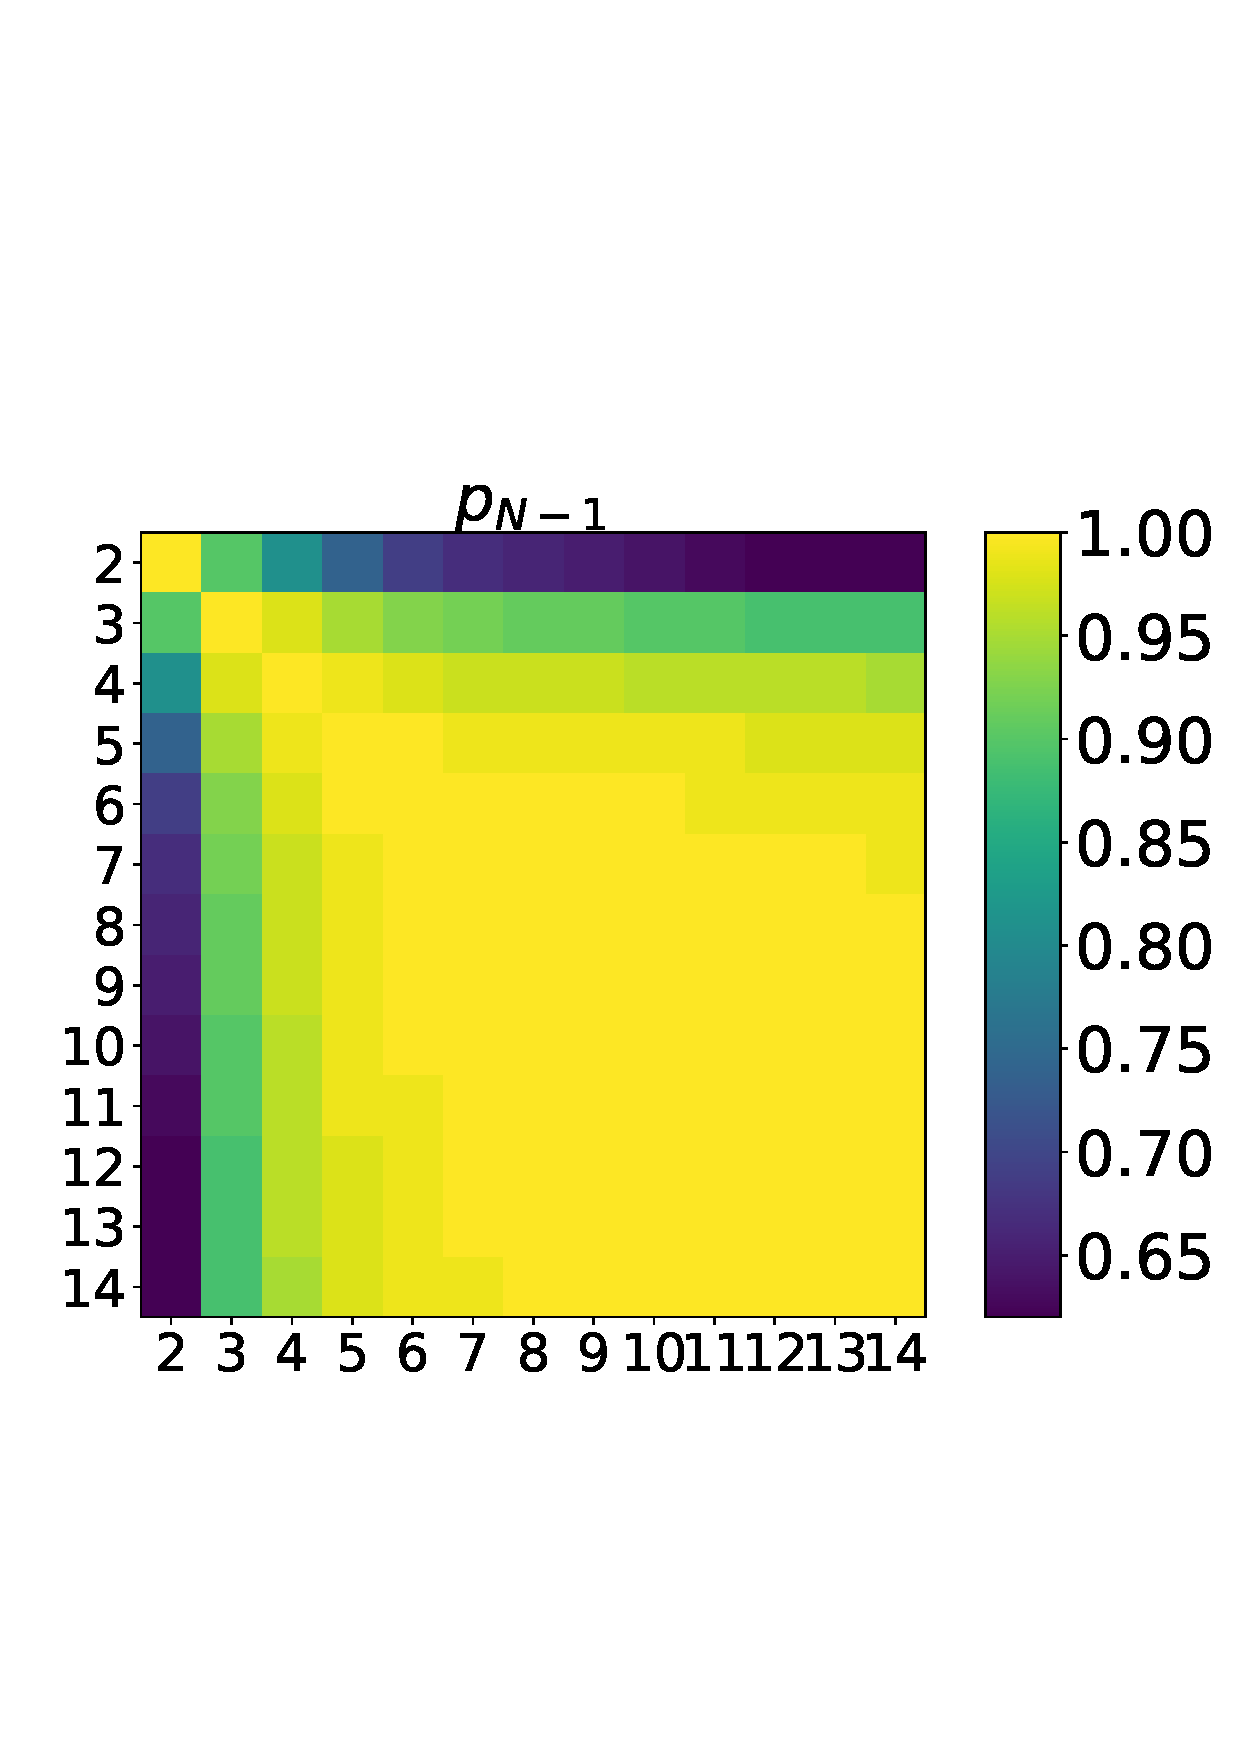
\includegraphics[width=\columnwidth]{./correlation_heatmap_resist.pdf}
        \caption{Rank based on \(x_{N - 1}\)}
    \end{subfigure}
    ~
    \begin{subfigure}[t]{.3\columnwidth}
        \centering
        \includegraphics[width=\columnwidth]{./correlation_heatmap_coexist.pdf}
        \caption{Rank based on \(x_{N/2}\)}
    \end{subfigure}
    \caption{Heatmap of correlation coefficients of rankings by population size.}
    \label{fig:correlation_coefficients}
\end{figure}


\section*{Discussion}

Training strategies to excel
at the Moran process leads to the evolution of cooperation, but only with like
individuals in the case of TF1 and TF2. This may have significant implications
for various biological and social phenomena such as
human social interactions, particularly the evolution of ingroup/outgroup mechanisms
and other sometimes costly rituals that reinforce group behavior.

While TF1 and TF2 are competent invaders, the best invaders
in the study do not appear to employ strict handshakes, and are generally
cooperative strategies. TF3, which does not use a handshake, is a better invader
than TF1 and TF2 but not as good a resistor. Nevertheless it was the result
of the same kind of training processes and is a better combined invader-resistor
than the invaders that were trained previously to maximize payout.

The strategies trained to maximize payoff in head-to-head matches are generally
cooperative and are effective invaders.
Combined with the fact that handshaking strategies are stronger resistors,
this suggests that while maximizing individual payoff can lead to the evolution
of cooperation, these strategies are not the most evolutionarily stable
in the long run. A strategy with a handshaking mechanism is still capable of
invading and is more resistant to subsequent invasions. Moreover, the
best resistor of the payoff maximally trained strategies (Evolved Looker Up
1\_1\_1),
which always defects if the opponent defects in the first round, is effectively
employing a one-shot handshake of C. Similarly, Grudger (also known as Grim),
which emerged from training memory one strategies for the Moran process,
also effectively employs a handshake of always cooperating, as it defects
for the remainder of the match if the opponent ever defects.

The insights that payoff maximizers are better invaders and that handshakers
are better resistors suggests that a strategy
aware of the population distribution could choose to become a handshaker at
a critical threshold and use a strategy better for invasion when in the
minority. Information about the population distribution was not available
to our strategies. Previous work has showed that strategies able to retain
memory across matches can infer the population distribution and act in such
a manner, resulting in a strategy effective at invasion and resistance
\cite{Lee2015}.

We did not attempt other objective functions that may serve to select for both
invasion and resistance better than training at a starting population of
$(N/2, N/2)$. Nevertheless our results suggest that there is not much room for
improvement. Any handshake more sophisticated than always cooperate necessarily involves
a defection. (A strategy with a handshake consisting of a long sequence of cooperations is
effectively a grudger.) For TF3 or EvolvedLookerUp1\_1\_1 to become better resistors
they need a longer or more strict handshake. But if this handshake involves
a defection then likely the invasion ability is diminished for $N > 2$: the top
invaders for larger $N$ are nice strategies that do not defect before their
opponents. This is because good invaders need to maximize match payoff to benefit
from fitness proportionate selection,
and so in the absence of a handshake mechanism, knowledge of the population
distribution, or some identifying label on the opponent,
a strategy must be generally cooperative. Aggressive strategies
are only effective invaders for the smallest $N$, dropping dramatically in rank
as the population size increases.

We did, however, attempt to evolve CS using finite state machines and lookup table
based players,
which resulted in some very similar strategies. In particular we evolved a
lookup strategy that had a handshake of DC and played TFT with other players
after a correct handshake while defecting otherwise, which is quite close in
function to CS (full grudging is not possible with a lookup table of limited
depth).

Finally we note that it may be possible to achieve similar results with smaller
capacity finite state machine players.

\section*{Conclusion}

A detailed empirical analysis of 164 strategies of the IPD within a pairwise
Moran process has been carried out. All \(\binom{164}{2}=13,366\) possible
ordered pairs of strategies have been placed in a Moran process with different
starting values allowing each strategy to attempt to invade the other.
This is the largest such experiment carried out and has led to many insights.

When studying evolutionary processes it is vital to consider \(N>2\) since
results for \(N=2\) cannot be used to extrapolate performance in larger
populations. This was shown both observationally
 but also by
considering the correlation of the ranks in different population sizes.

Memory one strategies do not perform as well as longer memory strategies in general
in this study. Several longer memory strategies were high performers for invasion,
particularly the strategies which have been trained using a number of reinforcement
learning algorithms. Interestingly they have been trained to perform well in
tournaments and not Moran processes specifically. In some cases these strategies
utilize all the history of play (the neural network strategies and the lookup
table strategies, the latter using the first round and some number of trailing rounds).

There are no memory one strategies in the top 5 performing strategies
for \(N>3\). Training memory-one strategies specifically for the Moran process
typically led to Grudger / Grim, a memory-one strategy with
four-vector (1, 0, 0, 0). It appears to be the best resistor of the memory-one strategies.
The highest performing memory-one strategy for invasion is PSO Gambler Mem 1,
training to maximize total payout, which has four-vector $(1, 0.52173487, 0, 0.12050939)$.
For comparison, training for maximum score difference between the player and the
opponent resulted in a strategy nearly the same as Grudger, with four-vector
$(0.9459, 0, 0, 0)$ (not included in the study).


One of the major findings discussed, is
the ability of strategies with a handshake mechanism to resist invasion. This
was not only revealed for CS (a human designed strategy) but also for
two FSM strategies (TF1 and TF2) specifically trained through an evolutionary
process. In these two cases, the handshake mechanism was a product of the
evolutionary process. Fig~\ref{fig:cooperation_rates} shows the cooperation
rate of TF1, TF2, TF3 and CS
for each round of a match against all the opponents in this study.
This corresponds to the fraction of cooperation played by that strategy observed
in a given round (out of the first 15) where each matchup is repeated 10000 times to
obtain the mean.

While TF3
does not have a strict handshake mechanism it is clear that all these strategies
start a match by cooperating. It is then evident that TF3 cooperates more than
the other strategies thus explaining the difference in performance. It is also
clear that CS only cooperates with itself and Handshake: it is a very aggressive
strategy.

\begin{figure}[!hbtp]
    \centering
    \begin{subfigure}[t]{.5\columnwidth}
        \centering
        \includegraphics[width=\columnwidth]{./cooperation_0_0_10000_TF1_array.pdf}
        \caption{TF1}
    \end{subfigure}%
    ~
    \begin{subfigure}[t]{.5\columnwidth}
        \centering
        \includegraphics[width=\columnwidth]{./cooperation_0_0_10000_TF2_array.pdf}
        \caption{TF2}
    \end{subfigure}

    \begin{subfigure}[t]{.5\columnwidth}
        \centering
        \includegraphics[width=\columnwidth]{./cooperation_0_0_10000_TF3_array.pdf}
        \caption{TF3}
    \end{subfigure}%
    ~
    \begin{subfigure}[t]{.5\columnwidth}
        \centering
        \includegraphics[width=\columnwidth]{./cooperation_0_0_10000_CS_array.pdf}
        \caption{CS}
    \end{subfigure}
    \caption{Cooperation rate per round (over 10000 repetitions). Rows
        correspond to all the strategies considered in this work (ordered
    alphabetically by name). Columns correspond to round of an IPD match.}
    \label{fig:cooperation_rates}
\end{figure}

These findings are important for the ongoing understanding of
population dynamics and offer evidence for some of the shortcomings of low
memory which has started to be recognised by the community \cite{Hilbe2017}.

All source code for this work has been written in a sustainable manner: it is
open source, under version control and tested which ensures that all results can
be reproduced \cite{Prlic2012, Sandve2013, Wilson2014}. The raw data as well as
the processed data has also been properly archived and can be found
at \cite{data}.

There are many opportunities to build on this work. In particular, an analysis
of the effect of noise should offer insights regarding the stability of the findings,
particularly for the handshaking strategies. They may be less dominant for
larger amounts of noise since the handshaking mechanisms may become brittle.
There are many other variations to explore including populations with more
than one type, spatial structure, and mutation.

One final point to recognise: the large set of strategies used here does not in
itself constitute an authoritative set. Whilst it is not only large but also very
diverse, the results (and rankings) presented might change given a different set
of strategies. A further piece of work could look at subgroups of strategies and
how they fair against other subgroups. Note that because of the open nature of
the work here (not only is the source code archived but so is the data) this and
any other further analysis is possible to carry out.


\section*{Acknowledgements}

This work was performed using the computational facilities of the Advanced
Research Computing @ Cardiff (ARCCA) Division, Cardiff University.

A variety of software libraries have been used in this work:

\begin{itemize}
    \item The Axelrod library (IPD strategies and Moran processes)
        \cite{axelrodproject}.
    \item The matplotlib library (visualisation) \cite{hunter2007matplotlib}.
    \item The pandas and numpy libraries (data manipulation)
        \cite{mckinney2010data, walt2011numpy}.
\end{itemize}

\nolinenumbers

\begin{thebibliography}{10}

\bibitem{Adami2013}
Christoph Adami and Arend Hintze.
\newblock {Evolutionary instability of zero-determinant strategies demonstrates
  that winning is not everything.}
\newblock {\em Nature communications}, 4(1):2193, 2013.

\bibitem{adami2016evolutionary}
Christoph Adami, Jory Schossau, and Arend Hintze.
\newblock {Evolutionary game theory using agent-based methods}.
\newblock {\em Physics of Life Reviews}, 19(Supplement C):1 -- 26, 2016.

\bibitem{affenzeller2009genetic}
Michael Affenzeller, Stefan Wagner, Stephan Winkler, and Andreas Beham.
\newblock {\em Genetic Algorithms and Genetic Programming: Modern Concepts and
  Practical Applications}.
\newblock Numerical Insights. CRC Press, 2009.

\bibitem{Nowak2017}
Benjamin Allen, Gabor Lippner, Yu-Ting Chen, Babak Fotouhi, Naghmeh Momeni,
  Shing-Tung Yau, and Martin~A Nowak.
\newblock {Evolutionary dynamics on any population structure}.
\newblock 544:227--230, March 2017.

\bibitem{Ashlock2015}
Daniel Ashlock, Joseph~Alexander Brown, and Philip Hingston.
\newblock {Multiple Opponent Optimization of Prisoner’s Dilemma Playing
  Agents}.
\newblock {\em IEEE Transactions on Computational Intelligence and AI in
  Games}, 7(1):53--65, 2015.

\bibitem{Ashlock2008}
Daniel Ashlock and Eun-Youn Kim.
\newblock {Fingerprinting: Visualization and automatic analysis of prisoner's
  dilemma strategies}.
\newblock {\em IEEE Transactions on Evolutionary Computation}, 12(5):647--659,
  2008.

\bibitem{Ashlock2006}
Wendy Ashlock and Daniel Ashlock.
\newblock {Changes in prisoner’s dilemma strategies over evolutionary time
  with different population sizes}.
\newblock In {\em Evolutionary Computation, 2006. CEC 2006. IEEE Congress on},
  pages 297--304. IEEE, 2006.

\bibitem{Ashlock2014}
Wendy Ashlock, Jeffrey Tsang, and Daniel Ashlock.
\newblock {The evolution of exploitation}.
\newblock In {\em Foundations of Computational Intelligence (FOCI), 2014 IEEE
  Symposium on}, pages 135--142. IEEE, 2014.

\bibitem{Axelrod1980a}
Robert Axelrod.
\newblock {Effective choice in the prisoner's dilemma}.
\newblock {\em Journal of conflict resolution}, 24(1):3--25, 1980.

\bibitem{Axelrod1980b}
Robert Axelrod.
\newblock {More Effective Choice in the Prisoner's Dilemma}.
\newblock {\em Journal of Conflict Resolution}, 24(3):379--403, 1980.

\bibitem{Axelrod1984}
Robert Axelrod.
\newblock {\em The Evolution of Cooperation}.
\newblock Basic books. Basic Books, 1984.

\bibitem{Baek2016}
{Baek, Seung Ki and Jeong, Hyeong-chai and Hilbe, Christian and Nowak, Martin
  A}.
\newblock {Comparing reactive and memory- one strategies of direct
  reciprocity}.
\newblock {\em Nature Publishing Group}, pages 1--13, 2016.

\bibitem{Banks1990}
Jeffrey~S Banks and Rangarajan~K Sundaram.
\newblock {Repeated games, finite automata, and complexity}.
\newblock {\em Games and Economic Behavior}, 2(2):97--117, 1990.

\bibitem{Beaufils1997}
Bruno Beaufils, Jean-Paul Delahaye, and Philippe Mathieu.
\newblock {Our meeting with gradual, a good strategy for the iterated
  prisoner’s dilemma}.
\newblock In {\em Proceedings of the Fifth International Workshop on the
  Synthesis and Simulation of Living Systems}, pages 202--209, 1997.

\bibitem{brown2001interval}
Lawrence~D Brown, T~Tony Cai, and Anirban DasGupta.
\newblock Interval estimation for a binomial proportion.
\newblock {\em Statistical science}, pages 101--117, 2001.

\bibitem{Andre2013}
Andre~LC Carvalho, Honovan~P Rocha, Felipe~T Amaral, and Frederico~G Guimaraes.
\newblock {Iterated Prisoner’s Dilemma-An extended analysis}.
\newblock pages 1--6, 2013.

\bibitem{Eckhart2015}
Arnold Eckhart.
\newblock Coopsim v0.9.9 beta 6.
\newblock https://github.com/jecki/CoopSim/, 2015.

\bibitem{Flood1958}
Merrill~M Flood.
\newblock {Some Experimental Games}, 1958.

\bibitem{Frean1994}
Marcus~R Frean.
\newblock {The prisoner's dilemma without synchrony}.
\newblock {\em Proceedings of the Royal Society of London B: Biological
  Sciences}, 257(1348):75--79, 1994.

\bibitem{Gaudesi2016}
Marco Gaudesi, Elio Piccolo, Giovanni Squillero, and Alberto Tonda.
\newblock {Exploiting evolutionary modeling to prevail in iterated prisoner’s
  dilemma tournaments}.
\newblock {\em IEEE Transactions on Computational Intelligence and AI in
  Games}, 8(3):288--300, 2016.

\bibitem{marc_harper_2017_824264}
Marc Harper, Vince Knight, and Martin Jones.
\newblock Axelrod-python/axelrod-dojo: v0.0.1.
\newblock https://doi.org/10.5281/zenodo.824264, July 2017.

\bibitem{Harper2017}
Marc Harper, Vincent Knight, Martin Jones, Georgios Koutsovoulos, Nikoleta~E
  Glynatsi, and Owen Campbell.
\newblock {Reinforcement Learning Produces Dominant Strategies for the Iterated
  Prisoner's Dilemma}.
\newblock arXiv:1707.06307, 2017.

\bibitem{Hilbe2017}
Christian Hilbe, Luis~A Martinez-Vaquero, Krishnendu Chatterjee, and Martin~A
  Nowak.
\newblock {Memory-n strategies of direct reciprocity}.
\newblock {\em Proceedings of the National Academy of Sciences}, page
  201621239, 2017.

\bibitem{Hilbe2013}
Christian Hilbe, Martin~A Nowak, and Arne Traulsen.
\newblock {Adaptive dynamics of extortion and compliance}.
\newblock {\em PloS one}, 8(11):e77886, 2013.

\bibitem{hunter2007matplotlib}
John~D Hunter.
\newblock {Matplotlib: A 2D graphics environment}.
\newblock {\em Computing In Science \& Engineering}, 9(3):90--95, 2007.

\bibitem{kendall2007iterated}
Graham Kendall, Xin Yao, and Siang~Y Chong.
\newblock {\em The Iterated Prisoners' Dilemma: 20 Years on}.
\newblock Advances in natural computation. World Scientific, 2007.

\bibitem{Knight2016}
Vincent Knight, Owen Campbell, Marc Harper, Karol~M Langner, James Campbell,
  Thomas Campbell, Alex Carney, Martin Chorley, Cameron Davidson-pilon,
  Nikoleta Glynatsi, Tom{\'{a}}{\v{s}} Ehrlich, Martin Jones, Georgios
  Koutsovoulos, Jochen Muller, Geraint Palmer, Piotr Petunov, Paul Slavin,
  Timothy Standen, Luis Visintini, and Karl Molden.
\newblock {An Open Framework for the Reproducible Study of the Iterated
  Prisoner ' s Dilemma}.
\newblock 2016.

\bibitem{data}
Vincent Knight, Marc Harper, and Nikoleta~E Glynatsi.
\newblock {Data for: Evolution Reinforces Cooperation with the Emergence of
  Self-Recognition Mechanisms: an empirical study of the Moran process for the
  iterated Prisoner's dilemma using reinforcement learning}.
\newblock https://doi.org/10.5281/zenodo.1040129, July 2017.

\bibitem{Kraines1989}
David Kraines and Vivian Kraines.
\newblock {Pavlov and the prisoner's dilemma}.
\newblock {\em Theory and decision}, 26(1):47--79, 1989.

\bibitem{Kuhn2017}
Steven Kuhn.
\newblock Prisoner's dilemma.
\newblock In Edward~N. Zalta, editor, {\em The Stanford Encyclopedia of
  Philosophy}. Metaphysics Research Lab, Stanford University, spring 2017
  edition, 2017.

\bibitem{Lee2015}
Christopher Lee, Marc Harper, and Dashiell Fryer.
\newblock {The Art of War: Beyond Memory-one Strategies in Population Games}.
\newblock {\em Plos One}, 10(3):e0120625, 2015.

\bibitem{Li2011}
Jiawei Li, Philip Hingston, and Graham Kendall.
\newblock {Engineering Design of Strategies for Winning Iterated Prisoner's
  Dilemma Competitions}.
\newblock {\em IEEE Transactions on Computational Intelligence and AI in
  Games}, 3(4):348--360, 2011.

\bibitem{Li2009}
Jiawei Li and Graham Kendall.
\newblock {A strategy with novel evolutionary features for the iterated
  prisoner's dilemma.}
\newblock {\em Evolutionary Computation}, 17(2):257--274, 2009.

\bibitem{Li2014}
Jiawei Li and Graham Kendall.
\newblock {The effect of memory size on the evolutionary stability of
  strategies in iterated prisoner's dilemma}.
\newblock {\em IEEE Transactions on Evolutionary Computation}, 18(6):819--826,
  2014.

\bibitem{Prison1998}
LIFL.
\newblock Prison.
\newblock http://www.lifl.fr/IPD/ipd.frame.html, 2008.

\bibitem{Mathieu2015}
Philippe Mathieu and Jean-Paul Delahaye.
\newblock {New Winning Strategies for the Iterated Prisoner's Dilemma (Extended
  Abstract)}.
\newblock {\em 14th International Conference on Autonomous Agents and
  Multiagent Systems (AAMAS 2015)}, pages 1665--1666, 2015.

\bibitem{mckinney2010data}
Wes McKinney et~al.
\newblock Data structures for statistical computing in python.
\newblock In {\em Proceedings of the 9th Python in Science Conference}, volume
  445, pages 51--56. van der Voort S, Millman J, 2010.

\bibitem{Mittal2009}
Shashi Mittal and Kalyanmoy Deb.
\newblock {Optimal strategies of the iterated prisoner's dilemma problem for
  multiple conflicting objectives}.
\newblock {\em IEEE Transactions on Evolutionary Computation}, 13(3):554--565,
  2009.

\bibitem{Moran1957}
Patrick A~P Moran.
\newblock {Random Processes in Genetics}.
\newblock {\em Mathematical Proceedings of the Cambridge Philosophical
  Society}, 54(1):60--71, 1957.

\bibitem{Nachbar1992}
John~H Nachbar.
\newblock {Evolution in the finitely repeated prisoner's dilemma}.
\newblock {\em Journal of Economic Behavior \& Organization}, 19(3):307--326,
  1992.

\bibitem{Nowak}
Martin~A Nowak.
\newblock {\em Evolutionary Dynamics: Exploring the Equations of Life}.
\newblock Cambridge: Harvard University Press.

\bibitem{Nowak1993}
Martin~A Nowak and Karl Sigmund.
\newblock {A strategy of win-stay, lose-shift that outperforms tit-for-tat in
  the Prisoner's Dilemma game.}
\newblock {\em Nature}, 364(6432):56--58, 1993.

\bibitem{Press2012}
William~H Press and Freeman~J Dyson.
\newblock {Iterated Prisoner's Dilemma contains strategies that dominate any
  evolutionary opponent.}
\newblock {\em Proceedings of the National Academy of Sciences of the United
  States of America}, 109(26):10409--13, 2012.

\bibitem{Prlic2012}
Andreas Prlić and James~B Procter.
\newblock {Ten Simple Rules for the Open Development of Scientific Software}.
\newblock {\em PLOS Computational Biology}, 8(12):1--3, 12 2012.

\bibitem{axelrodproject}
The~Axelrod project developers.
\newblock Axelrod: v2.9.0.
\newblock http://dx.doi.org/10.5281/zenodo.499122, April 2016.

\bibitem{Robson1990}
Arthur~J Robson.
\newblock {Efficiency in evolutionary games: Darwin, Nash and the secret
  handshake}.
\newblock {\em Journal of theoretical Biology}, 144(3):379--396, 1990.

\bibitem{Sandve2013}
Geir~Kjetil Sandve, Anton Nekrutenko, James Taylor, and Eivind Hovig.
\newblock {Ten Simple Rules for Reproducible Computational Research}.
\newblock {\em PLoS Computational Biology}, 9(10):1--4, 2013.

\bibitem{Stewart2012}
Alexander~J Stewart and Joshua~B Plotkin.
\newblock {Extortion and cooperation in the Prisoner’s Dilemma}.
\newblock {\em Proceedings of the National Academy of Sciences},
  109(26):10134--10135, 2012.

\bibitem{stewart2013extortion}
Alexander~J Stewart and Joshua~B Plotkin.
\newblock {From extortion to generosity, evolution in the iterated prisoner’s
  dilemma}.
\newblock {\em Proceedings of the National Academy of Sciences},
  110(38):15348--15353, 2013.

\bibitem{Tzafestas2000}
Elpida Tzafestas.
\newblock {Toward adaptive cooperative behavior}.
\newblock {\em From Animals to animals: Proceedings of the 6th International
  Conference on the Simulation of Adaptive Behavior {(SAB-2000)}}, 2:334--340,
  2000.

\bibitem{PD2017}
Unkwown.
\newblock www.prisoners-dilemma.com.
\newblock http://www.prisoners-dilemma.com/, 2017.

\bibitem{Berg2015}
Pieter Van~den Berg and Franz~J Weissing.
\newblock {The importance of mechanisms for the evolution of cooperation}.
\newblock In {\em Proc. R. Soc. B}, volume 282, page 20151382. The Royal
  Society, 2015.

\bibitem{walt2011numpy}
St{\'e}fan van~der Walt, S~Chris Colbert, and Gael Varoquaux.
\newblock {The NumPy array: a structure for efficient numerical computation}.
\newblock {\em Computing in Science \& Engineering}, 13(2):22--30, 2011.

\bibitem{West2016}
Jeffrey West, Zaki Hasnain, Jeremy Mason, and Paul~K Newton.
\newblock {The prisoner’s dilemma as a cancer model}.
\newblock {\em Convergent Science Physical Oncology}, 2(3):035002, 2016.

\bibitem{Wilson2014}
Greg Wilson, D~A Aruliah, C~Titus Brown, Neil~P Chue~Hong, Matt Davis,
  Richard~T Guy, Steven H~D Haddock, Kathryn~D Huff, Ian~M Mitchell, Mark~D
  Plumbley, Ben Waugh, Ethan~P White, and Paul Wilson.
\newblock {Best Practices for Scientific Computing}.
\newblock {\em PLOS Biology}, 12(1):1--7, 01 2014.

\bibitem{Axelrod1995}
Jianzhong Wu and Robert Axelrod.
\newblock {How to cope with noise in the iterated prisoner's dilemma}.
\newblock {\em Journal of Conflict resolution}, 39(1):183--189, 1995.

\end{thebibliography}

\appendix

\section{Appendix A: List of players}\label{app:list_of_players}

\footnotesize
\begin{enumerate}
\item $\phi$ - \textit{Deterministic} - \textit{Memory depth}: \(\infty\). \cite{axelrodproject}
\item $\pi$ - \textit{Deterministic} - \textit{Memory depth}: \(\infty\). \cite{axelrodproject}
\item $e$ - \textit{Deterministic} - \textit{Memory depth}: \(\infty\). \cite{axelrodproject}
\item ALLCorALLD - \textit{Stochastic} - \textit{Memory depth}: 1. \cite{axelrodproject}
\item Adaptive - \textit{Deterministic} - \textit{Memory depth}: \(\infty\). \cite{Li2011}
\item Adaptive Pavlov 2006 - \textit{Deterministic} - \textit{Memory depth}: \(\infty\). \cite{kendall2007iterated}
\item Adaptive Pavlov 2011 - \textit{Deterministic} - \textit{Memory depth}: \(\infty\). \cite{Li2011}
\item Adaptive Tit For Tat: 0.5 - \textit{Deterministic} - \textit{Memory depth}: \(\infty\). \cite{Tzafestas2000}
\item Aggravater - \textit{Deterministic} - \textit{Memory depth}: \(\infty\). \cite{axelrodproject}
\item Alternator - \textit{Deterministic} - \textit{Memory depth}: 1. \cite{Axelrod1984, Mittal2009}
\item Alternator Hunter - \textit{Deterministic} - \textit{Memory depth}: \(\infty\). \cite{axelrodproject}
\item Anti Tit For Tat - \textit{Deterministic} - \textit{Memory depth}: 1. \cite{Hilbe2013}
\item AntiCycler - \textit{Deterministic} - \textit{Memory depth}: \(\infty\). \cite{axelrodproject}
\item Appeaser - \textit{Deterministic} - \textit{Memory depth}: \(\infty\). \cite{axelrodproject}
\item Arrogant QLearner - \textit{Stochastic} - \textit{Memory depth}: \(\infty\). \cite{axelrodproject}
\item Average Copier - \textit{Stochastic} - \textit{Memory depth}: \(\infty\). \cite{axelrodproject}
\item Better and Better - \textit{Stochastic} - \textit{Memory depth}: \(\infty\). \cite{Prison1998}
\item Bully - \textit{Deterministic} - \textit{Memory depth}: 1. \cite{Nachbar1992}
\item Calculator - \textit{Stochastic} - \textit{Memory depth}: \(\infty\). \cite{Prison1998}
\item Cautious QLearner - \textit{Stochastic} - \textit{Memory depth}: \(\infty\). \cite{axelrodproject}
\item CollectiveStrategy(\textbf{CS}) - \textit{Deterministic} - \textit{Memory depth}: \(\infty\). \cite{Li2009}
\item Contrite Tit For Tat(\textbf{CTfT}) - \textit{Deterministic} - \textit{Memory depth}: 3. \cite{Axelrod1995}
\item Cooperator - \textit{Deterministic} - \textit{Memory depth}: 0. \cite{Axelrod1984, Mittal2009, Press2012}
\item Cooperator Hunter - \textit{Deterministic} - \textit{Memory depth}: \(\infty\). \cite{axelrodproject}
\item Cycle Hunter - \textit{Deterministic} - \textit{Memory depth}: \(\infty\). \cite{axelrodproject}
\item Cycler CCCCCD - \textit{Deterministic} - \textit{Memory depth}: 5. \cite{axelrodproject}
\item Cycler CCCD - \textit{Deterministic} - \textit{Memory depth}: 3. \cite{axelrodproject}
\item Cycler CCCDCD - \textit{Deterministic} - \textit{Memory depth}: 5. \cite{axelrodproject}
\item Cycler CCD - \textit{Deterministic} - \textit{Memory depth}: 2. \cite{Mittal2009}
\item Cycler DC - \textit{Deterministic} - \textit{Memory depth}: 1. \cite{axelrodproject}
\item Cycler DDC - \textit{Deterministic} - \textit{Memory depth}: 2. \cite{Mittal2009}
\item Davis: 10 - \textit{Deterministic} - \textit{Memory depth}: \(\infty\). \cite{Axelrod1980a}
\item Defector - \textit{Deterministic} - \textit{Memory depth}: 0. \cite{Axelrod1984, Mittal2009, Press2012}
\item Defector Hunter - \textit{Deterministic} - \textit{Memory depth}: \(\infty\). \cite{axelrodproject}
\item Desperate - \textit{Stochastic} - \textit{Memory depth}: 1. \cite{Berg2015}
\item Doubler - \textit{Deterministic} - \textit{Memory depth}: \(\infty\). \cite{Prison1998}
\item EasyGo - \textit{Deterministic} - \textit{Memory depth}: \(\infty\). \cite{Li2011, Prison1998}
\item Eatherley - \textit{Stochastic} - \textit{Memory depth}: \(\infty\). \cite{Axelrod1980b}
\item Eventual Cycle Hunter - \textit{Deterministic} - \textit{Memory depth}: \(\infty\). \cite{axelrodproject}
\item Evolved ANN - \textit{Deterministic} - \textit{Memory depth}: \(\infty\). \cite{axelrodproject}
\item Evolved ANN 5 - \textit{Deterministic} - \textit{Memory depth}: \(\infty\). \cite{axelrodproject}
\item Evolved ANN 5 Noise 05 - \textit{Deterministic} - \textit{Memory depth}: \(\infty\). \cite{axelrodproject}
\item Evolved FSM 16 - \textit{Deterministic} - \textit{Memory depth}: 16 - \textit{Number of states}: 14. \cite{axelrodproject}
\item Evolved FSM 16 Noise 05 - \textit{Deterministic} - \textit{Memory depth}: 16 - \textit{Number of states}: 14. \cite{axelrodproject}
\item Evolved FSM 4 - \textit{Deterministic} - \textit{Memory depth}: 4 - \textit{Number of states}: 4. \cite{axelrodproject}
\item Evolved HMM 5 - \textit{Stochastic} - \textit{Memory depth}: 5. \cite{axelrodproject}
\item EvolvedLookerUp1\_1\_1 - \textit{Deterministic} - \textit{Memory depth}: \(\infty\). \cite{axelrodproject}
\item EvolvedLookerUp2\_2\_2 - \textit{Deterministic} - \textit{Memory depth}: \(\infty\). \cite{axelrodproject}
\item FSM Player: [(0, 'C', 0, 'C'), (0, 'D', 3, 'C'), (1, 'C', 5, 'D'), (1, 'D', 0, 'C'), (2, 'C', 3, 'C'), (2, 'D', 2, 'D'), (3, 'C', 4, 'D'), (3, 'D', 6, 'D'), (4, 'C', 3, 'C'), (4, 'D', 1, 'D'), (5, 'C', 6, 'C'), (5, 'D', 3, 'D'), (6, 'C', 6, 'D'), (6, 'D', 6, 'D'), (7, 'C', 7, 'D'), (7, 'D', 5, 'C')], 0, C(\textbf{TF3}) - \textit{Deterministic} - \textit{Memory depth}: \(\infty\) - \textit{Number of states}: 8.
\item FSM Player: [(0, 'C', 13, 'D'), (0, 'D', 12, 'D'), (1, 'C', 3, 'D'), (1, 'D', 4, 'D'), (2, 'C', 14, 'D'), (2, 'D', 9, 'D'), (3, 'C', 0, 'C'), (3, 'D', 1, 'D'), (4, 'C', 1, 'D'), (4, 'D', 2, 'D'), (5, 'C', 12, 'C'), (5, 'D', 6, 'C'), (6, 'C', 1, 'C'), (6, 'D', 14, 'D'), (7, 'C', 12, 'D'), (7, 'D', 2, 'D'), (8, 'C', 7, 'D'), (8, 'D', 9, 'D'), (9, 'C', 8, 'D'), (9, 'D', 0, 'D'), (10, 'C', 2, 'C'), (10, 'D', 15, 'C'), (11, 'C', 7, 'D'), (11, 'D', 13, 'D'), (12, 'C', 3, 'C'), (12, 'D', 8, 'D'), (13, 'C', 7, 'C'), (13, 'D', 10, 'D'), (14, 'C', 10, 'D'), (14, 'D', 7, 'D'), (15, 'C', 15, 'C'), (15, 'D', 11, 'D')], 0, C(\textbf{TF2}) - \textit{Deterministic} - \textit{Memory depth}: \(\infty\) - \textit{Number of states}: 16.
\item FSM Player: [(0, 'C', 7, 'C'), (0, 'D', 1, 'C'), (1, 'C', 11, 'D'), (1, 'D', 11, 'D'), (2, 'C', 8, 'D'), (2, 'D', 8, 'C'), (3, 'C', 3, 'C'), (3, 'D', 12, 'D'), (4, 'C', 6, 'C'), (4, 'D', 3, 'C'), (5, 'C', 11, 'C'), (5, 'D', 8, 'D'), (6, 'C', 13, 'D'), (6, 'D', 14, 'C'), (7, 'C', 4, 'D'), (7, 'D', 2, 'D'), (8, 'C', 14, 'D'), (8, 'D', 8, 'D'), (9, 'C', 0, 'C'), (9, 'D', 10, 'D'), (10, 'C', 8, 'C'), (10, 'D', 15, 'C'), (11, 'C', 6, 'D'), (11, 'D', 5, 'D'), (12, 'C', 6, 'D'), (12, 'D', 9, 'D'), (13, 'C', 9, 'D'), (13, 'D', 8, 'D'), (14, 'C', 8, 'D'), (14, 'D', 13, 'D'), (15, 'C', 4, 'C'), (15, 'D', 5, 'C')], 0, C(\textbf{TF1}) - \textit{Deterministic} - \textit{Memory depth}: \(\infty\) - \textit{Number of states}: 16.
\item Feld: 1.0, 0.5, 200 - \textit{Stochastic} - \textit{Memory depth}: 200. \cite{Axelrod1980a}
\item Firm But Fair - \textit{Stochastic} - \textit{Memory depth}: 1. \cite{Frean1994}
\item Fool Me Forever - \textit{Deterministic} - \textit{Memory depth}: \(\infty\). \cite{axelrodproject}
\item Fool Me Once - \textit{Deterministic} - \textit{Memory depth}: \(\infty\). \cite{axelrodproject}
\item Forgetful Fool Me Once: 0.05 - \textit{Stochastic} - \textit{Memory depth}: \(\infty\). \cite{axelrodproject}
\item Forgetful Grudger - \textit{Deterministic} - \textit{Memory depth}: 10. \cite{axelrodproject}
\item Forgiver - \textit{Deterministic} - \textit{Memory depth}: \(\infty\). \cite{axelrodproject}
\item Forgiving Tit For Tat(\textbf{FTfT}) - \textit{Deterministic} - \textit{Memory depth}: \(\infty\). \cite{axelrodproject}
\item Fortress3 - \textit{Deterministic} - \textit{Memory depth}: 3 - \textit{Number of states}: 3. \cite{Ashlock2006}
\item Fortress4 - \textit{Deterministic} - \textit{Memory depth}: 4 - \textit{Number of states}: 4. \cite{Ashlock2006}
\item GTFT: 0.33 - \textit{Stochastic} - \textit{Memory depth}: 1. \cite{Gaudesi2016, Nowak1993}
\item General Soft Grudger: n=1,d=4,c=2 - \textit{Deterministic} - \textit{Memory depth}: \(\infty\). \cite{axelrodproject}
\item Gradual - \textit{Deterministic} - \textit{Memory depth}: \(\infty\). \cite{Beaufils1997}
\item Gradual Killer: ('D', 'D', 'D', 'D', 'D', 'C', 'C') - \textit{Deterministic} - \textit{Memory depth}: \(\infty\). \cite{Prison1998}
\item Grofman - \textit{Stochastic} - \textit{Memory depth}: \(\infty\). \cite{Axelrod1980a}
\item Grudger - \textit{Deterministic} - \textit{Memory depth}: 1. \cite{Axelrod1980a, Banks1990, Beaufils1997, Berg2015, Li2011}
\item GrudgerAlternator - \textit{Deterministic} - \textit{Memory depth}: \(\infty\). \cite{Prison1998}
\item Grumpy: Nice, 10, -10 - \textit{Deterministic} - \textit{Memory depth}: \(\infty\). \cite{axelrodproject}
\item Handshake - \textit{Deterministic} - \textit{Memory depth}: \(\infty\). \cite{Robson1990}
\item Hard Go By Majority - \textit{Deterministic} - \textit{Memory depth}: \(\infty\). \cite{Mittal2009}
\item Hard Go By Majority: 10 - \textit{Deterministic} - \textit{Memory depth}: 10. \cite{axelrodproject}
\item Hard Go By Majority: 20 - \textit{Deterministic} - \textit{Memory depth}: 20. \cite{axelrodproject}
\item Hard Go By Majority: 40 - \textit{Deterministic} - \textit{Memory depth}: 40. \cite{axelrodproject}
\item Hard Go By Majority: 5 - \textit{Deterministic} - \textit{Memory depth}: 5. \cite{axelrodproject}
\item Hard Prober - \textit{Deterministic} - \textit{Memory depth}: \(\infty\). \cite{Prison1998}
\item Hard Tit For 2 Tats(\textbf{HTf2T}) - \textit{Deterministic} - \textit{Memory depth}: 3. \cite{Stewart2012}
\item Hard Tit For Tat(\textbf{HTfT}) - \textit{Deterministic} - \textit{Memory depth}: 3. \cite{PD2017}
\item Hesitant QLearner - \textit{Stochastic} - \textit{Memory depth}: \(\infty\). \cite{axelrodproject}
\item Hopeless - \textit{Stochastic} - \textit{Memory depth}: 1. \cite{Berg2015}
\item Inverse - \textit{Stochastic} - \textit{Memory depth}: \(\infty\). \cite{axelrodproject}
\item Inverse Punisher - \textit{Deterministic} - \textit{Memory depth}: \(\infty\). \cite{axelrodproject}
\item Joss: 0.9 - \textit{Stochastic} - \textit{Memory depth}: 1. \cite{Axelrod1980a, Stewart2012}
\item Level Punisher - \textit{Deterministic} - \textit{Memory depth}: \(\infty\). \cite{Eckhart2015}
\item Limited Retaliate 2: 0.08, 15 - \textit{Deterministic} - \textit{Memory depth}: \(\infty\). \cite{axelrodproject}
\item Limited Retaliate 3: 0.05, 20 - \textit{Deterministic} - \textit{Memory depth}: \(\infty\). \cite{axelrodproject}
\item Limited Retaliate: 0.1, 20 - \textit{Deterministic} - \textit{Memory depth}: \(\infty\). \cite{axelrodproject}
\item MEM2 - \textit{Deterministic} - \textit{Memory depth}: \(\infty\). \cite{Li2014}
\item Math Constant Hunter - \textit{Deterministic} - \textit{Memory depth}: \(\infty\). \cite{axelrodproject}
\item Meta Hunter Aggressive: 7 players - \textit{Deterministic} - \textit{Memory depth}: \(\infty\). \cite{axelrodproject}
\item Meta Hunter: 6 players - \textit{Deterministic} - \textit{Memory depth}: \(\infty\). \cite{axelrodproject}
\item Naive Prober: 0.1 - \textit{Stochastic} - \textit{Memory depth}: 1. \cite{Li2011}
\item Negation - \textit{Stochastic} - \textit{Memory depth}: 1. \cite{PD2017}
\item Nice Average Copier - \textit{Stochastic} - \textit{Memory depth}: \(\infty\). \cite{axelrodproject}
\item Nydegger - \textit{Deterministic} - \textit{Memory depth}: 3. \cite{Axelrod1980a}
\item Omega TFT: 3, 8 - \textit{Deterministic} - \textit{Memory depth}: \(\infty\). \cite{kendall2007iterated}
\item Once Bitten - \textit{Deterministic} - \textit{Memory depth}: 12. \cite{axelrodproject}
\item Opposite Grudger - \textit{Deterministic} - \textit{Memory depth}: \(\infty\). \cite{axelrodproject}
\item PSO Gambler 1\_1\_1 - \textit{Stochastic} - \textit{Memory depth}: \(\infty\). \cite{axelrodproject}
\item PSO Gambler 2\_2\_2 - \textit{Stochastic} - \textit{Memory depth}: \(\infty\). \cite{axelrodproject}
\item PSO Gambler 2\_2\_2 Noise 05 - \textit{Stochastic} - \textit{Memory depth}: \(\infty\). \cite{axelrodproject}
\item PSO Gambler Mem1 - \textit{Stochastic} - \textit{Memory depth}: 1. \cite{axelrodproject}
\item Predator - \textit{Deterministic} - \textit{Memory depth}: 9 - \textit{Number of states}: 9. \cite{Ashlock2006}
\item Prober - \textit{Deterministic} - \textit{Memory depth}: \(\infty\). \cite{Li2011}
\item Prober 2 - \textit{Deterministic} - \textit{Memory depth}: \(\infty\). \cite{Prison1998}
\item Prober 3 - \textit{Deterministic} - \textit{Memory depth}: \(\infty\). \cite{Prison1998}
\item Prober 4 - \textit{Deterministic} - \textit{Memory depth}: \(\infty\). \cite{Prison1998}
\item Pun1 - \textit{Deterministic} - \textit{Memory depth}: 2 - \textit{Number of states}: 2. \cite{Ashlock2006}
\item Punisher - \textit{Deterministic} - \textit{Memory depth}: \(\infty\). \cite{axelrodproject}
\item Raider - \textit{Deterministic} - \textit{Memory depth}: 3 - \textit{Number of states}: 4. \cite{Ashlock2014}
\item Random Hunter - \textit{Deterministic} - \textit{Memory depth}: \(\infty\). \cite{axelrodproject}
\item Random: 0.5 - \textit{Stochastic} - \textit{Memory depth}: 0. \cite{Axelrod1980a, Tzafestas2000}
\item Remorseful Prober: 0.1 - \textit{Stochastic} - \textit{Memory depth}: 2. \cite{Li2011}
\item Resurrection - \textit{Deterministic} - \textit{Memory depth}: 1. \cite{Eckhart2015}
\item Retaliate 2: 0.08 - \textit{Deterministic} - \textit{Memory depth}: \(\infty\). \cite{axelrodproject}
\item Retaliate 3: 0.05 - \textit{Deterministic} - \textit{Memory depth}: \(\infty\). \cite{axelrodproject}
\item Retaliate: 0.1 - \textit{Deterministic} - \textit{Memory depth}: \(\infty\). \cite{axelrodproject}
\item Revised Downing: True - \textit{Deterministic} - \textit{Memory depth}: \(\infty\). \cite{Axelrod1980a}
\item Ripoff - \textit{Deterministic} - \textit{Memory depth}: 2 - \textit{Number of states}: 3. \cite{Ashlock2008}
\item Risky QLearner - \textit{Stochastic} - \textit{Memory depth}: \(\infty\). \cite{axelrodproject}
\item SelfSteem - \textit{Stochastic} - \textit{Memory depth}: \(\infty\). \cite{Andre2013}
\item ShortMem - \textit{Deterministic} - \textit{Memory depth}: 10. \cite{Andre2013}
\item Shubik - \textit{Deterministic} - \textit{Memory depth}: \(\infty\). \cite{Axelrod1980a}
\item Slow Tit For Two Tats - \textit{Deterministic} - \textit{Memory depth}: 2. \cite{axelrodproject}
\item Slow Tit For Two Tats 2 - \textit{Deterministic} - \textit{Memory depth}: 2. \cite{Prison1998}
\item Sneaky Tit For Tat - \textit{Deterministic} - \textit{Memory depth}: \(\infty\). \cite{axelrodproject}
\item Soft Go By Majority - \textit{Deterministic} - \textit{Memory depth}: \(\infty\). \cite{Axelrod1984, Mittal2009}
\item Soft Go By Majority: 10 - \textit{Deterministic} - \textit{Memory depth}: 10. \cite{axelrodproject}
\item Soft Go By Majority: 20 - \textit{Deterministic} - \textit{Memory depth}: 20. \cite{axelrodproject}
\item Soft Go By Majority: 40 - \textit{Deterministic} - \textit{Memory depth}: 40. \cite{axelrodproject}
\item Soft Go By Majority: 5 - \textit{Deterministic} - \textit{Memory depth}: 5. \cite{axelrodproject}
\item Soft Grudger - \textit{Deterministic} - \textit{Memory depth}: 6. \cite{Li2011}
\item Soft Joss: 0.9 - \textit{Stochastic} - \textit{Memory depth}: 1. \cite{Prison1998}
\item SolutionB1 - \textit{Deterministic} - \textit{Memory depth}: 3 - \textit{Number of states}: 3. \cite{Ashlock2015}
\item SolutionB5 - \textit{Deterministic} - \textit{Memory depth}: 5 - \textit{Number of states}: 6. \cite{Ashlock2015}
\item Spiteful Tit For Tat - \textit{Deterministic} - \textit{Memory depth}: \(\infty\). \cite{Prison1998}
\item Stochastic Cooperator - \textit{Stochastic} - \textit{Memory depth}: 1. \cite{Adami2013}
\item Stochastic WSLS: 0.05 - \textit{Stochastic} - \textit{Memory depth}: 1. \cite{axelrodproject}
\item Suspicious Tit For Tat - \textit{Deterministic} - \textit{Memory depth}: 1. \cite{Beaufils1997, Hilbe2013}
\item Tester - \textit{Deterministic} - \textit{Memory depth}: \(\infty\). \cite{Axelrod1980b}
\item ThueMorse - \textit{Deterministic} - \textit{Memory depth}: \(\infty\). \cite{axelrodproject}
\item ThueMorseInverse - \textit{Deterministic} - \textit{Memory depth}: \(\infty\). \cite{axelrodproject}
\item Thumper - \textit{Deterministic} - \textit{Memory depth}: 2 - \textit{Number of states}: 2. \cite{Ashlock2008}
\item Tit For 2 Tats(\textbf{Tf2T}) - \textit{Deterministic} - \textit{Memory depth}: 2. \cite{Axelrod1984}
\item Tit For Tat(\textbf{TfT}) - \textit{Deterministic} - \textit{Memory depth}: 1. \cite{Axelrod1980a}
\item Tricky Cooperator - \textit{Deterministic} - \textit{Memory depth}: 10. \cite{axelrodproject}
\item Tricky Defector - \textit{Deterministic} - \textit{Memory depth}: \(\infty\). \cite{axelrodproject}
\item Tullock: 11 - \textit{Stochastic} - \textit{Memory depth}: 11. \cite{Axelrod1980a}
\item Two Tits For Tat(\textbf{2TfT}) - \textit{Deterministic} - \textit{Memory depth}: 2. \cite{Axelrod1984}
\item VeryBad - \textit{Deterministic} - \textit{Memory depth}: \(\infty\). \cite{Andre2013}
\item Willing - \textit{Stochastic} - \textit{Memory depth}: 1. \cite{Berg2015}
\item Win-Shift Lose-Stay: D(\textbf{WShLSt}) - \textit{Deterministic} - \textit{Memory depth}: 1. \cite{Li2011}
\item Win-Stay Lose-Shift: C(\textbf{WSLS}) - \textit{Deterministic} - \textit{Memory depth}: 1. \cite{Kraines1989, Nowak1993, Stewart2012}
\item Winner12 - \textit{Deterministic} - \textit{Memory depth}: 2. \cite{Mathieu2015}
\item Winner21 - \textit{Deterministic} - \textit{Memory depth}: 2. \cite{Mathieu2015}
\item Worse and Worse - \textit{Stochastic} - \textit{Memory depth}: \(\infty\). \cite{Prison1998}
\item Worse and Worse 2 - \textit{Stochastic} - \textit{Memory depth}: \(\infty\). \cite{Prison1998}
\item Worse and Worse 3 - \textit{Stochastic} - \textit{Memory depth}: \(\infty\). \cite{Prison1998}
\item ZD-Extort-2 v2: 0.125, 0.5, 1 - \textit{Stochastic} - \textit{Memory depth}: 1. \cite{Kuhn2017}
\item ZD-Extort-2: 0.1111111111111111, 0.5 - \textit{Stochastic} - \textit{Memory depth}: 1. \cite{Stewart2012}
\item ZD-Extort-4: 0.23529411764705882, 0.25, 1 - \textit{Stochastic} - \textit{Memory depth}: 1. \cite{axelrodproject}
\item ZD-GEN-2: 0.125, 0.5, 3 - \textit{Stochastic} - \textit{Memory depth}: 1. \cite{Kuhn2017}
\item ZD-GTFT-2: 0.25, 0.5 - \textit{Stochastic} - \textit{Memory depth}: 1. \cite{Stewart2012}
\item ZD-SET-2: 0.25, 0.0, 2 - \textit{Stochastic} - \textit{Memory depth}: 1. \cite{Kuhn2017}
\end{enumerate}

\section{Appendix B: Supplementary figures}

\begin{itemize}
    \item Figures~\ref{invasion-3}-\ref{invasion-14} show the fixation probability \(x_1\)
for each strategy. The mean and error bars are shown against the collection of
all opponents.

    \item Figures~\ref{resistance-3}-\ref{resistance-14} show the fixation probability
\(x_{N-1}\) for each strategy. Again, the mean and error bars are shown against
the collection of all opponents.

    \item Figures~\ref{fig:ranks_v_size_invade}-\ref{fig:ranks_v_size_coexist} show the
ranks of each strategy according to mean absorption probability across all
population sizes.
\end{itemize}

\begin{figure}[!hbtp]
    \centering
    \includegraphics[width=\textwidth]{./boxplot_3_invade.pdf}
    \caption{The fixation probabilities \(x_1\) for \(N=3\)}
    \label{invasion-3}
\end{figure}

\begin{figure}[!hbtp]
    \centering
    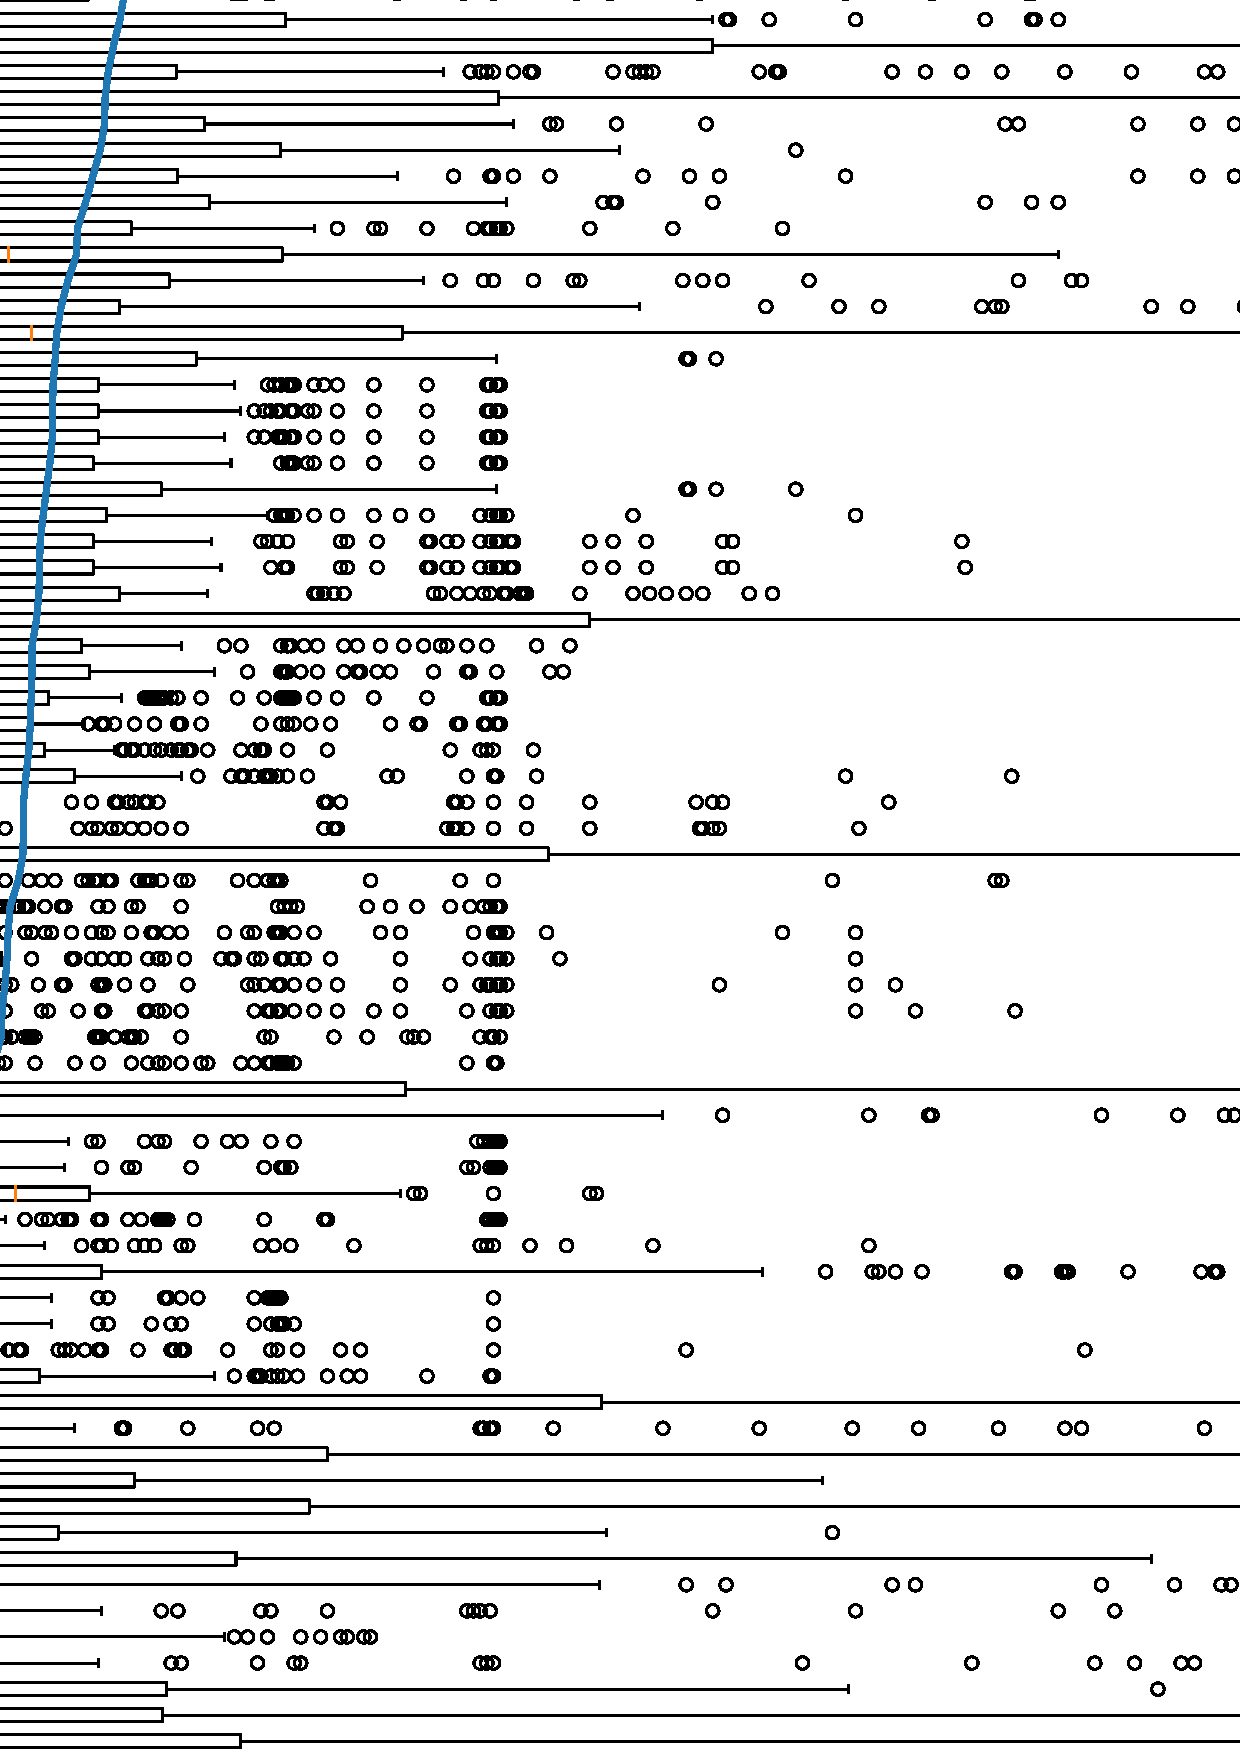
\includegraphics[width=\textwidth]{./boxplot_4_invade.pdf}
    \caption{The fixation probabilities \(x_1\) for \(N=4\)}
\end{figure}

\begin{figure}[!hbtp]
    \centering
    \includegraphics[width=\textwidth]{./boxplot_5_invade.pdf}
    \caption{The fixation probabilities \(x_1\) for \(N=5\)}
\end{figure}

\begin{figure}[!hbtp]
    \centering
    \includegraphics[width=\textwidth]{./boxplot_6_invade.pdf}
    \caption{The fixation probabilities \(x_1\) for \(N=6\)}
\end{figure}

\begin{figure}[!hbtp]
    \centering
    \includegraphics[width=\textwidth]{./boxplot_7_invade.pdf}
    \caption{The fixation probabilities \(x_1\) for \(N=7\)}
\end{figure}

\begin{figure}[!hbtp]
    \centering
    \includegraphics[width=\textwidth]{./boxplot_8_invade.pdf}
    \caption{The fixation probabilities \(x_1\) for \(N=8\)}
\end{figure}

\begin{figure}[!hbtp]
    \centering
    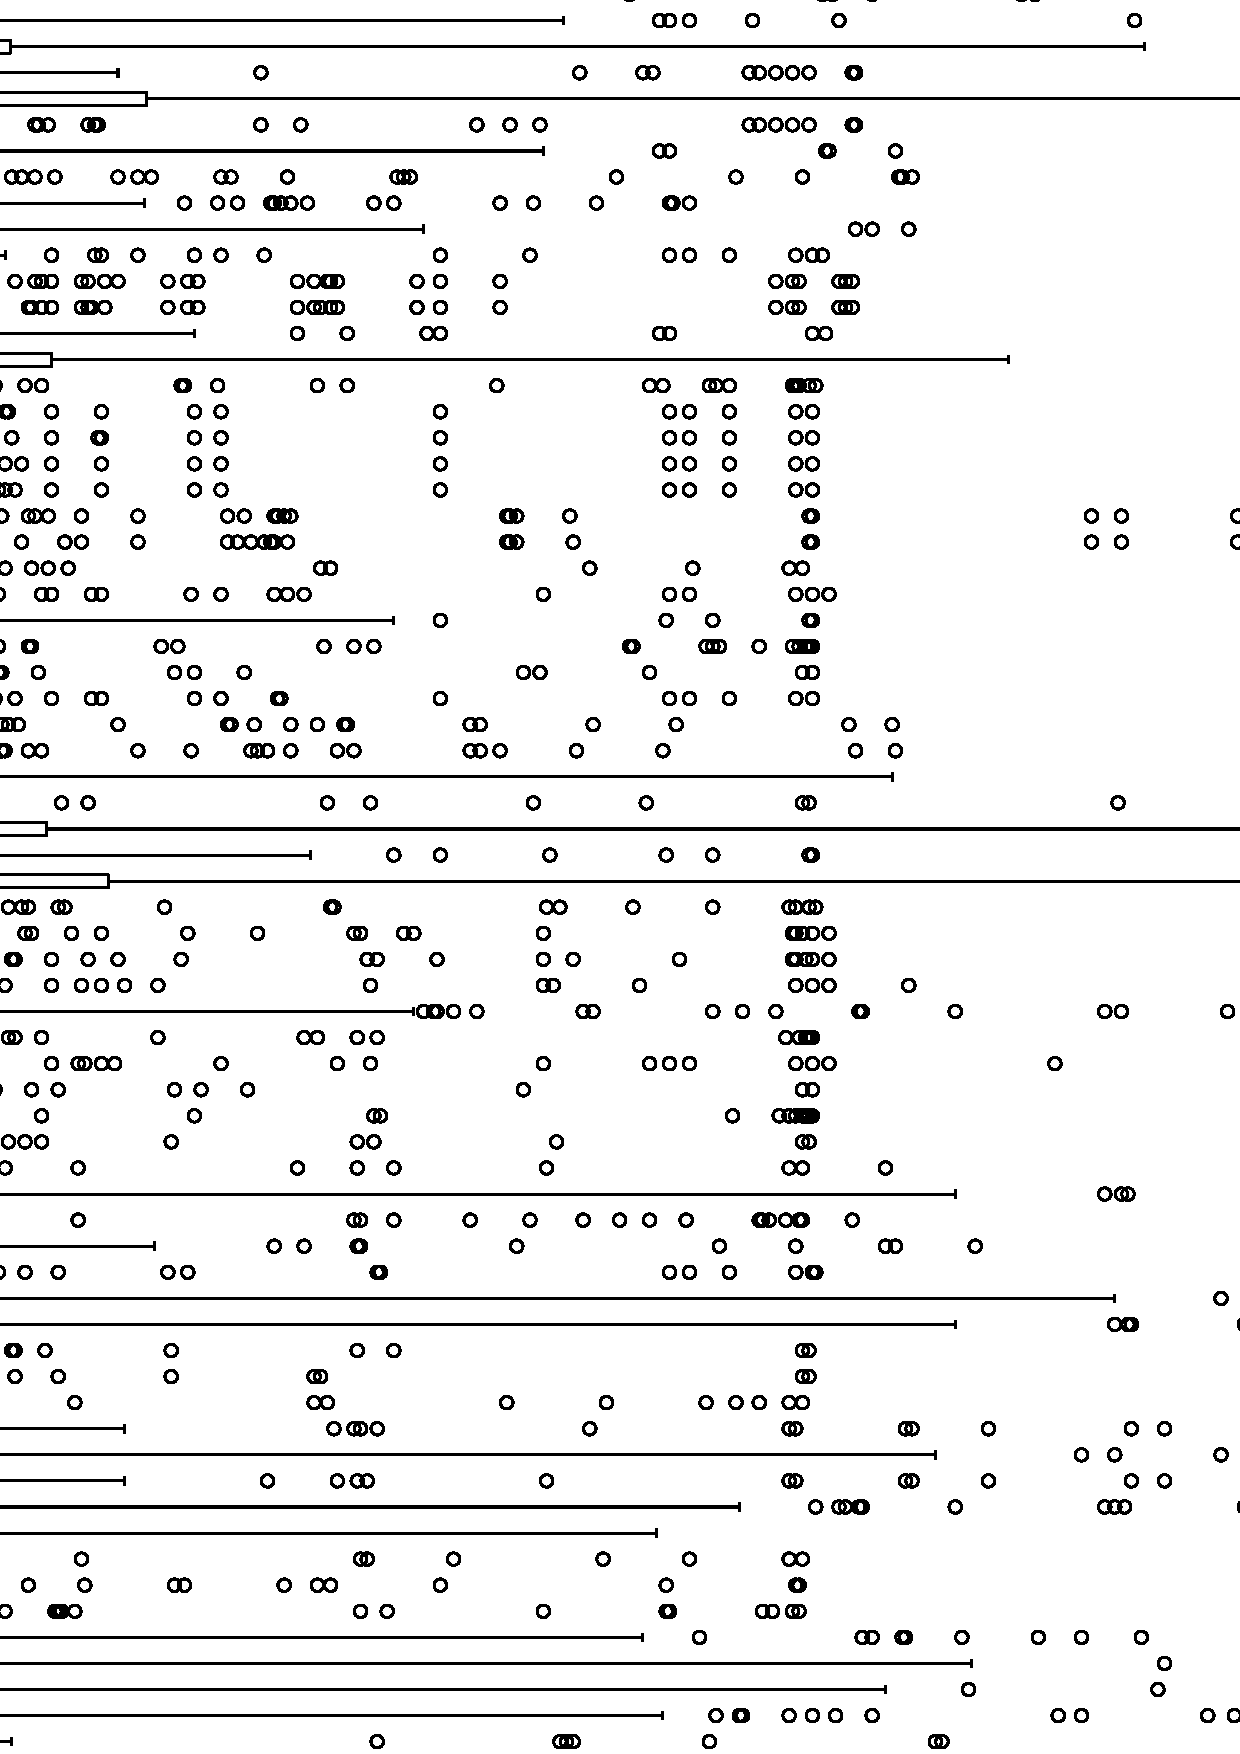
\includegraphics[width=\textwidth]{./boxplot_9_invade.pdf}
    \caption{The fixation probabilities \(x_1\) for \(N=9\)}
\end{figure}

\begin{figure}[!hbtp]
    \centering
    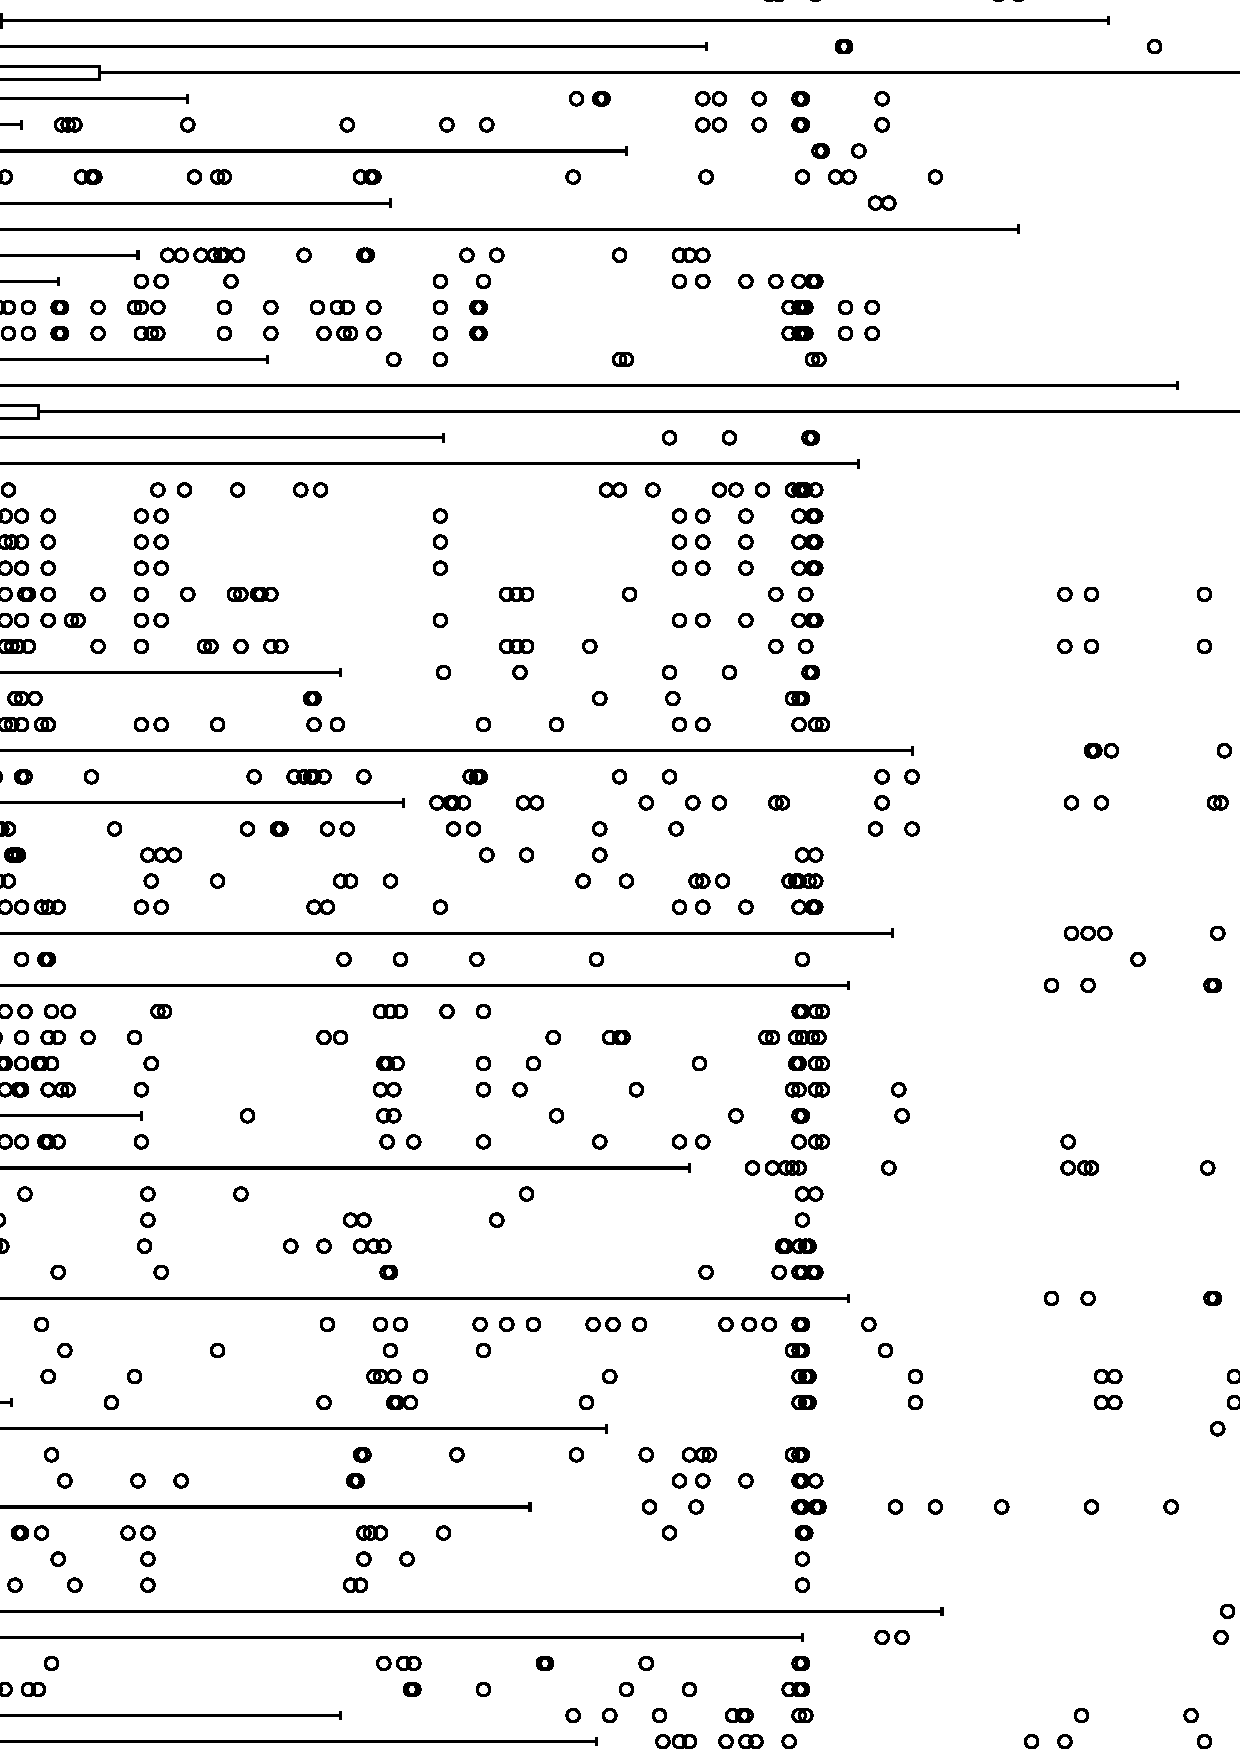
\includegraphics[width=\textwidth]{./boxplot_10_invade.pdf}
    \caption{The fixation probabilities \(x_1\) for \(N=10\)}
\end{figure}

\begin{figure}[!hbtp]
    \centering
    \includegraphics[width=\textwidth]{./boxplot_11_invade.pdf}
    \caption{The fixation probabilities \(x_1\) for \(N=11\)}
\end{figure}

\begin{figure}[!hbtp]
    \centering
    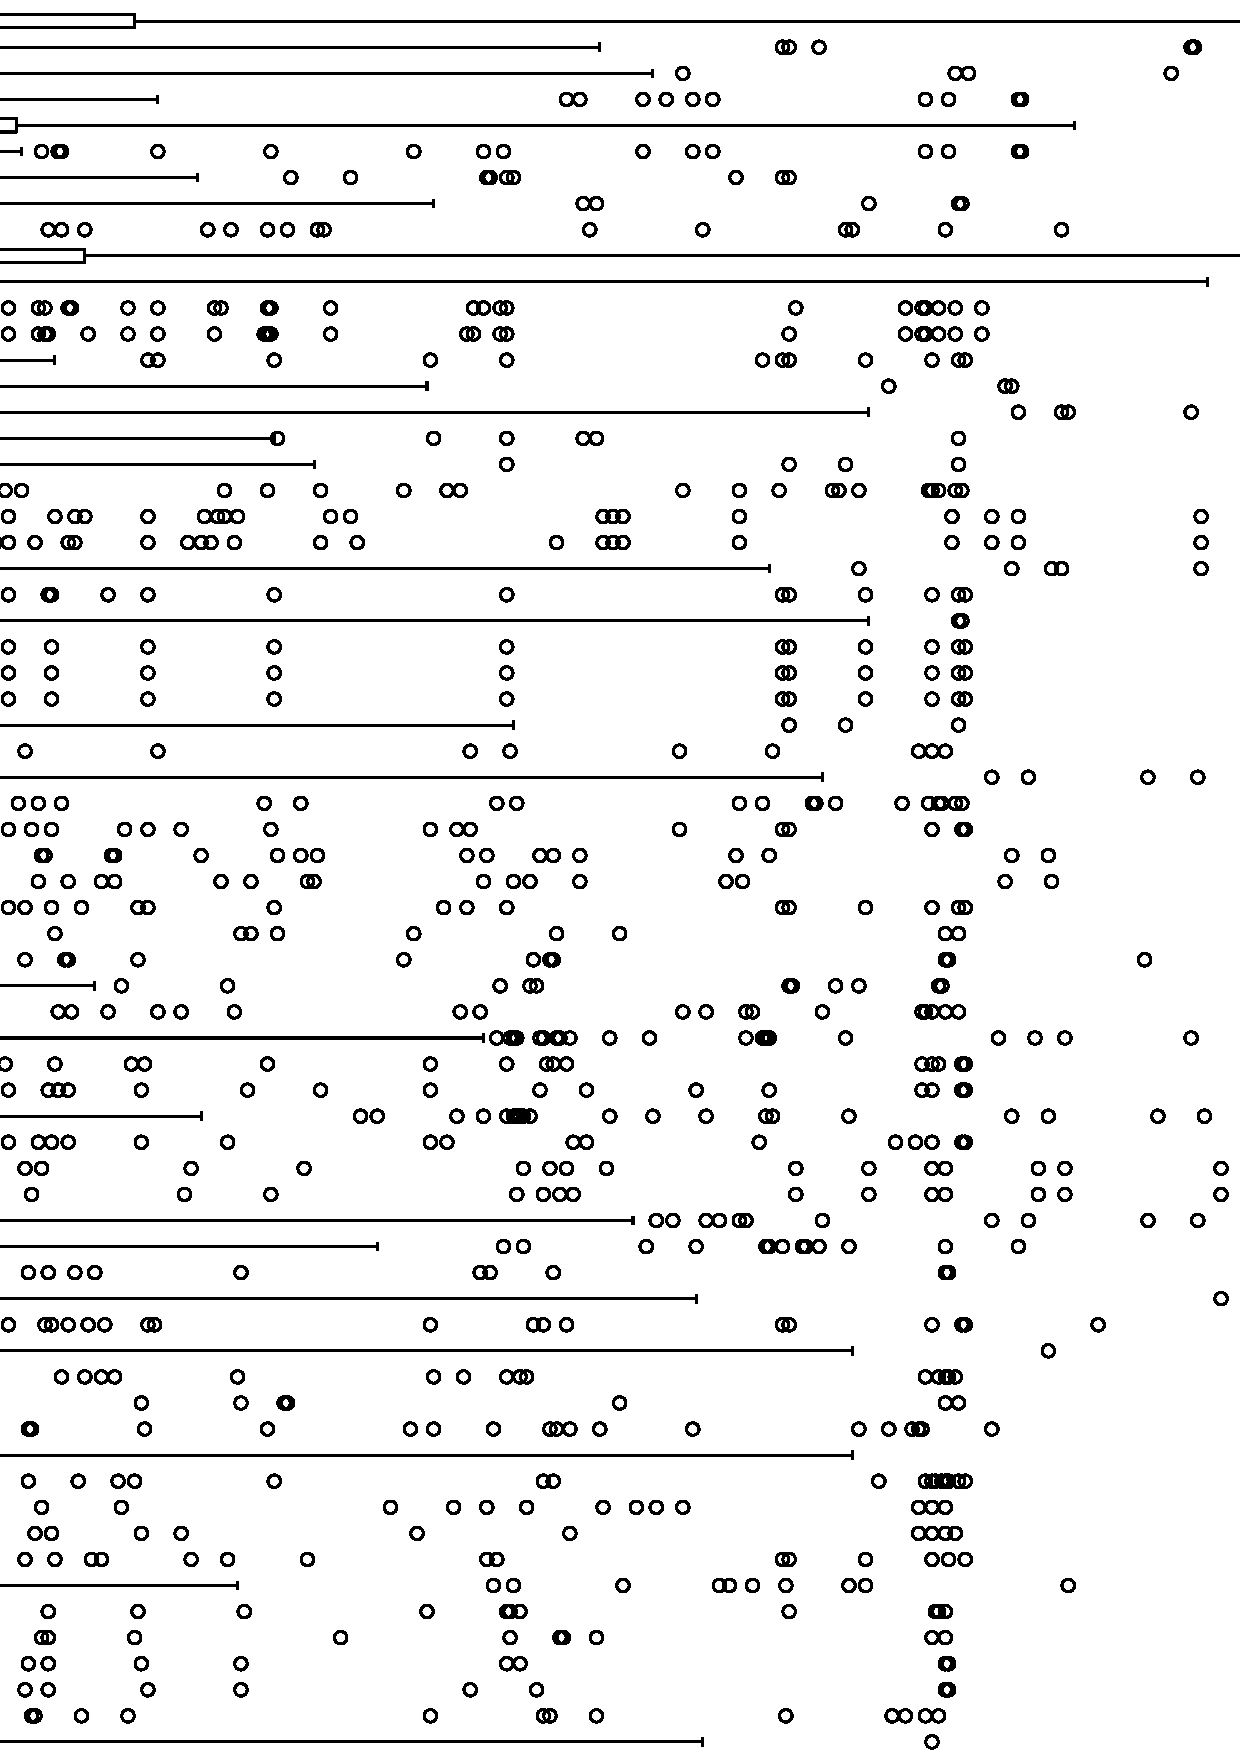
\includegraphics[width=\textwidth]{./boxplot_12_invade.pdf}
    \caption{The fixation probabilities \(x_1\) for \(N=12\)}
\end{figure}

\begin{figure}[!hbtp]
    \centering
    \includegraphics[width=\textwidth]{./boxplot_13_invade.pdf}
    \caption{The fixation probabilities \(x_1\) for \(N=13\)}
\end{figure}

\begin{figure}[!hbtp]
    \centering
    \includegraphics[width=\textwidth]{./boxplot_14_invade.pdf}
    \caption{The fixation probabilities \(x_1\) for \(N=14\)}
    \label{invasion-14}
\end{figure}


\begin{figure}[!hbtp]
    \centering
    \includegraphics[width=\textwidth]{./boxplot_3_resist.pdf}
    \caption{The fixation probabilities \(x_{N-1}\) for \(N=3\)}
    \label{resistance-3}
\end{figure}

\begin{figure}[!hbtp]
    \centering
    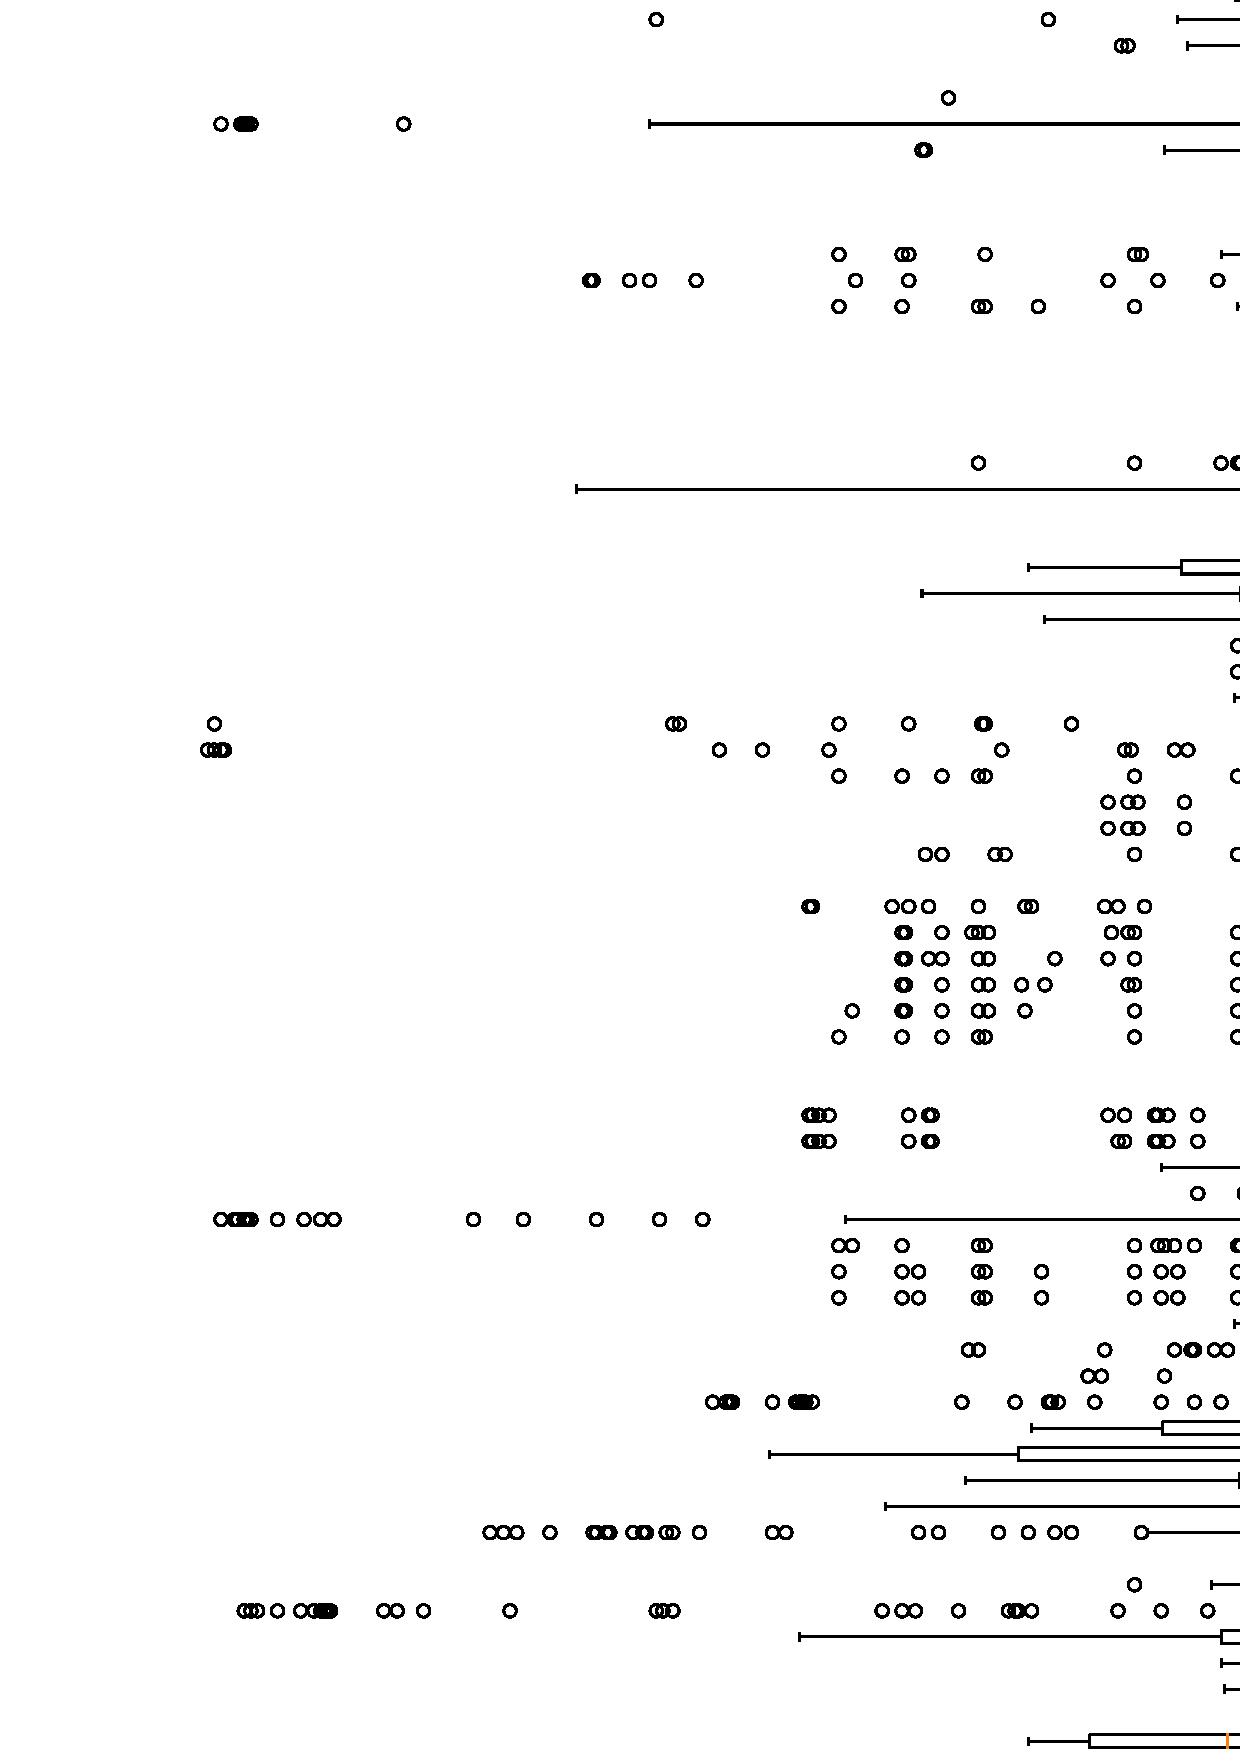
\includegraphics[width=\textwidth]{./boxplot_4_resist.pdf}
    \caption{The fixation probabilities \(x_{N-1}\) for \(N=4\)}
\end{figure}

\begin{figure}[!hbtp]
    \centering
    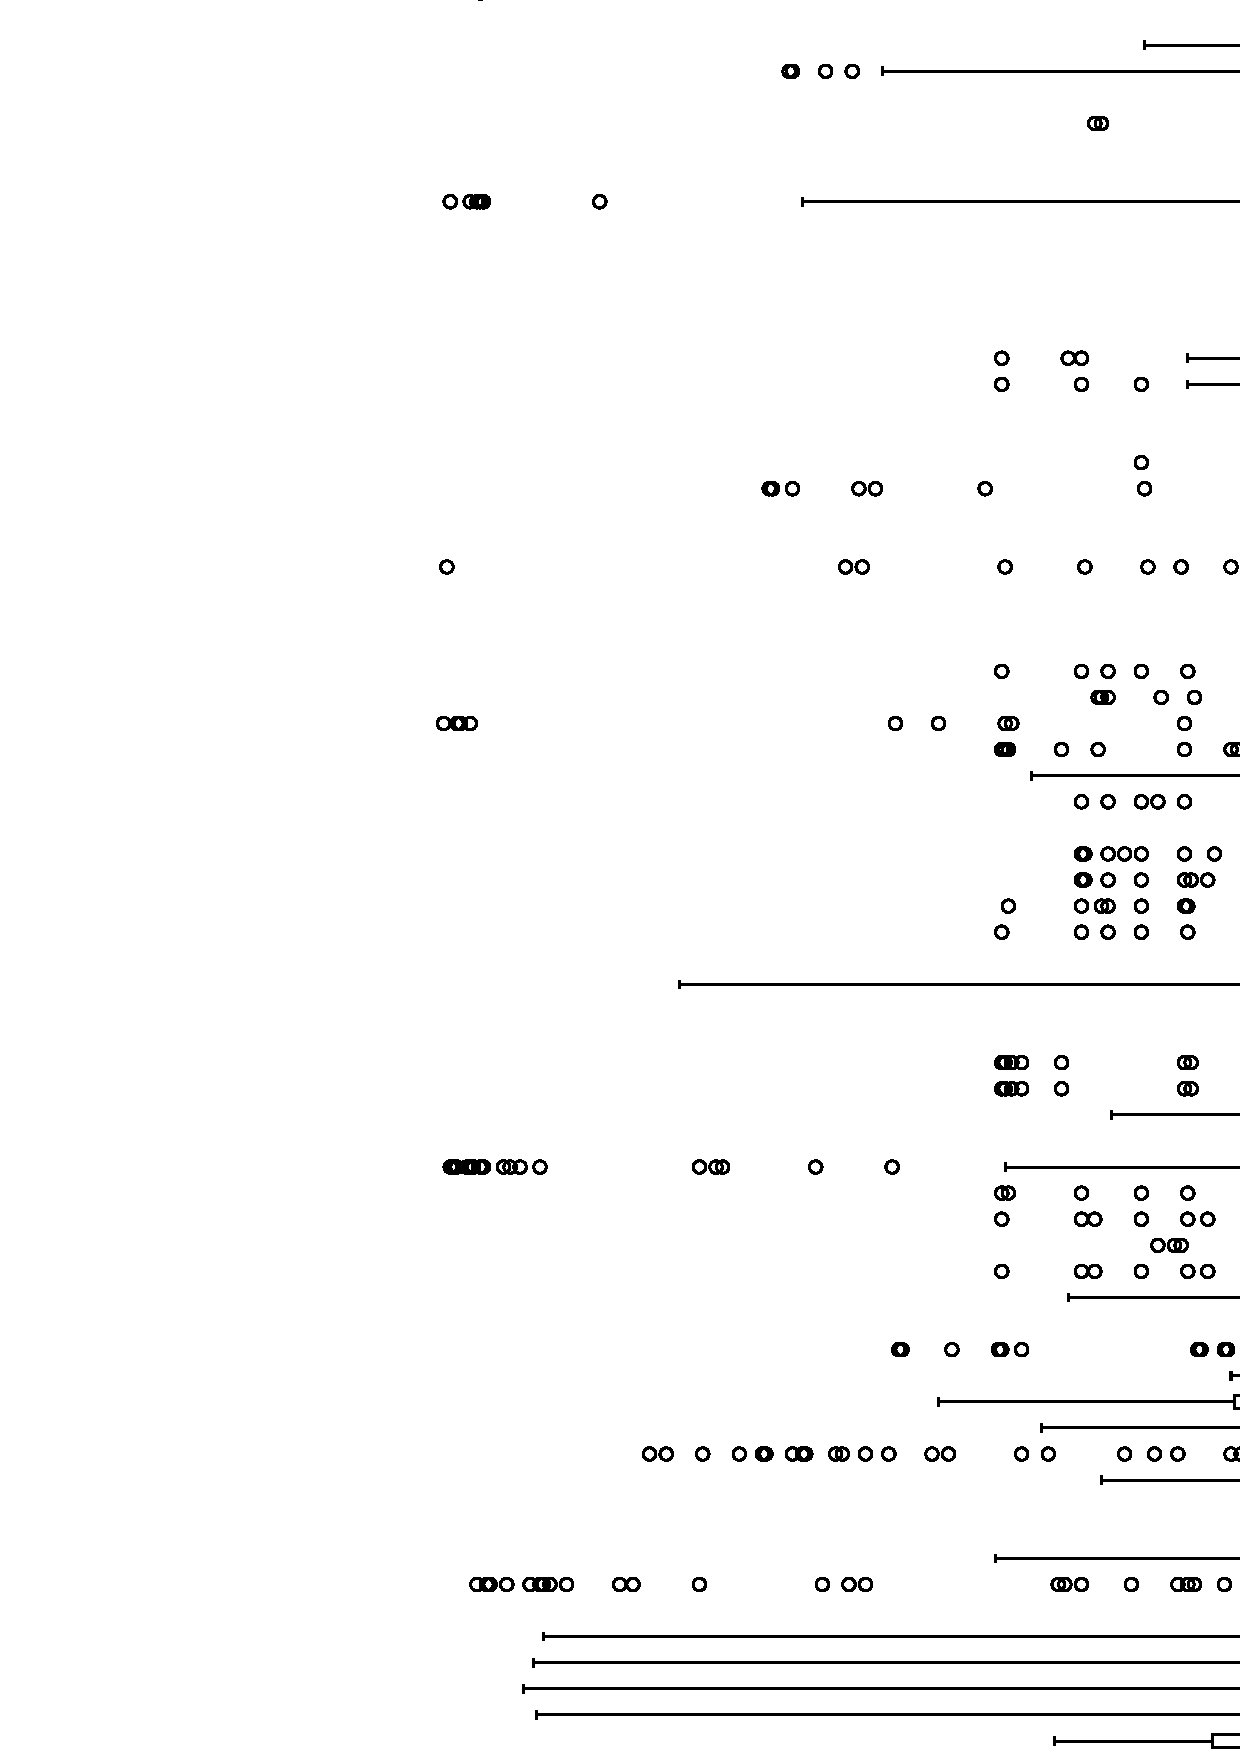
\includegraphics[width=\textwidth]{./boxplot_5_resist.pdf}
    \caption{The fixation probabilities \(x_{N-1}\) for \(N=5\)}
\end{figure}

\begin{figure}[!hbtp]
    \centering
    \includegraphics[width=\textwidth]{./boxplot_6_resist.pdf}
    \caption{The fixation probabilities \(x_{N-1}\) for \(N=6\)}
\end{figure}

\begin{figure}[!hbtp]
    \centering
    \includegraphics[width=\textwidth]{./boxplot_7_resist.pdf}
    \caption{The fixation probabilities \(x_{N-1}\) for \(N=7\)}
\end{figure}

\begin{figure}[!hbtp]
    \centering
    \includegraphics[width=\textwidth]{./boxplot_8_resist.pdf}
    \caption{The fixation probabilities \(x_{N-1}\) for \(N=8\)}
\end{figure}

\begin{figure}[!hbtp]
    \centering
    \includegraphics[width=\textwidth]{./boxplot_9_resist.pdf}
    \caption{The fixation probabilities \(x_{N-1}\) for \(N=9\)}
\end{figure}

\begin{figure}[!hbtp]
    \centering
    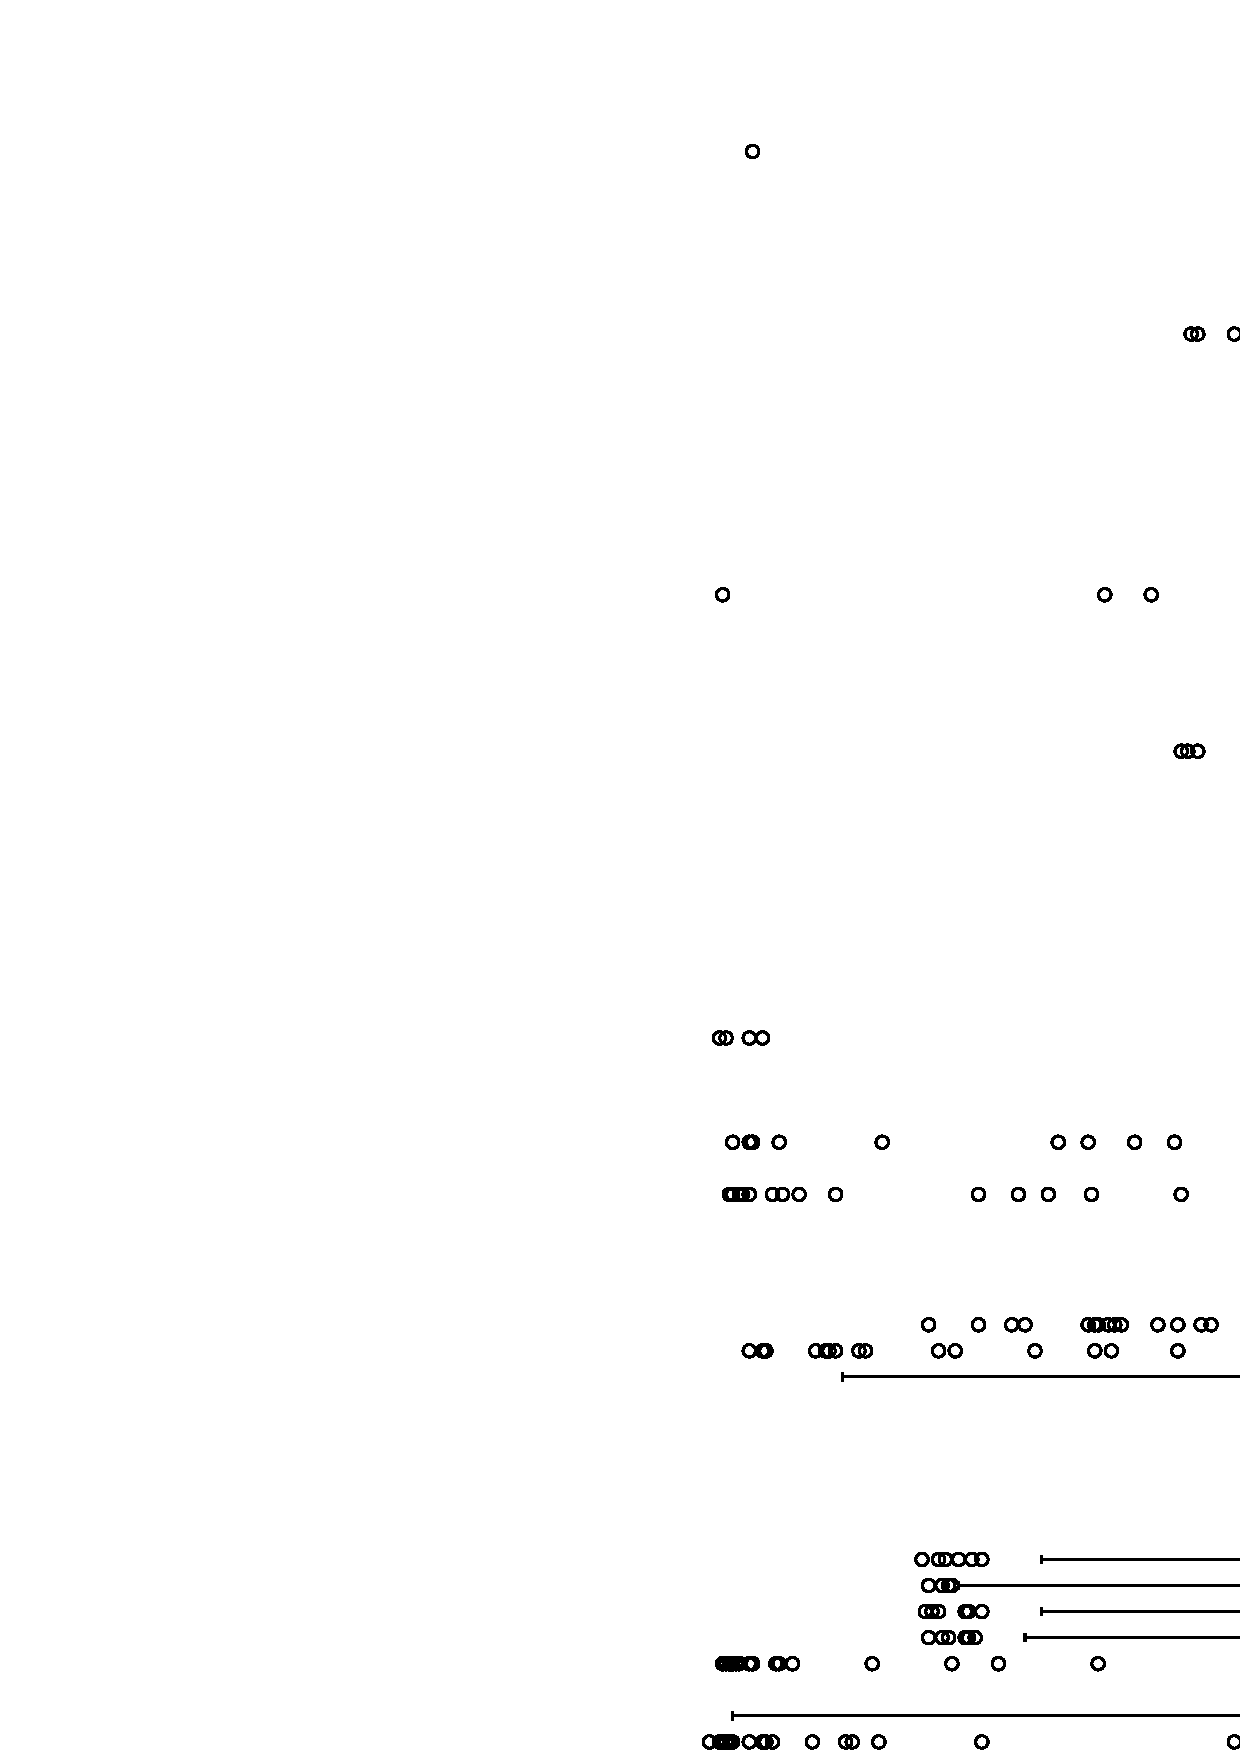
\includegraphics[width=\textwidth]{./boxplot_10_resist.pdf}
    \caption{The fixation probabilities \(x_{N-1}\) for \(N=10\)}
\end{figure}

\begin{figure}[!hbtp]
    \centering
    \includegraphics[width=\textwidth]{./boxplot_11_resist.pdf}
    \caption{The fixation probabilities \(x_{N-1}\) for \(N=11\)}
\end{figure}

\begin{figure}[!hbtp]
    \centering
    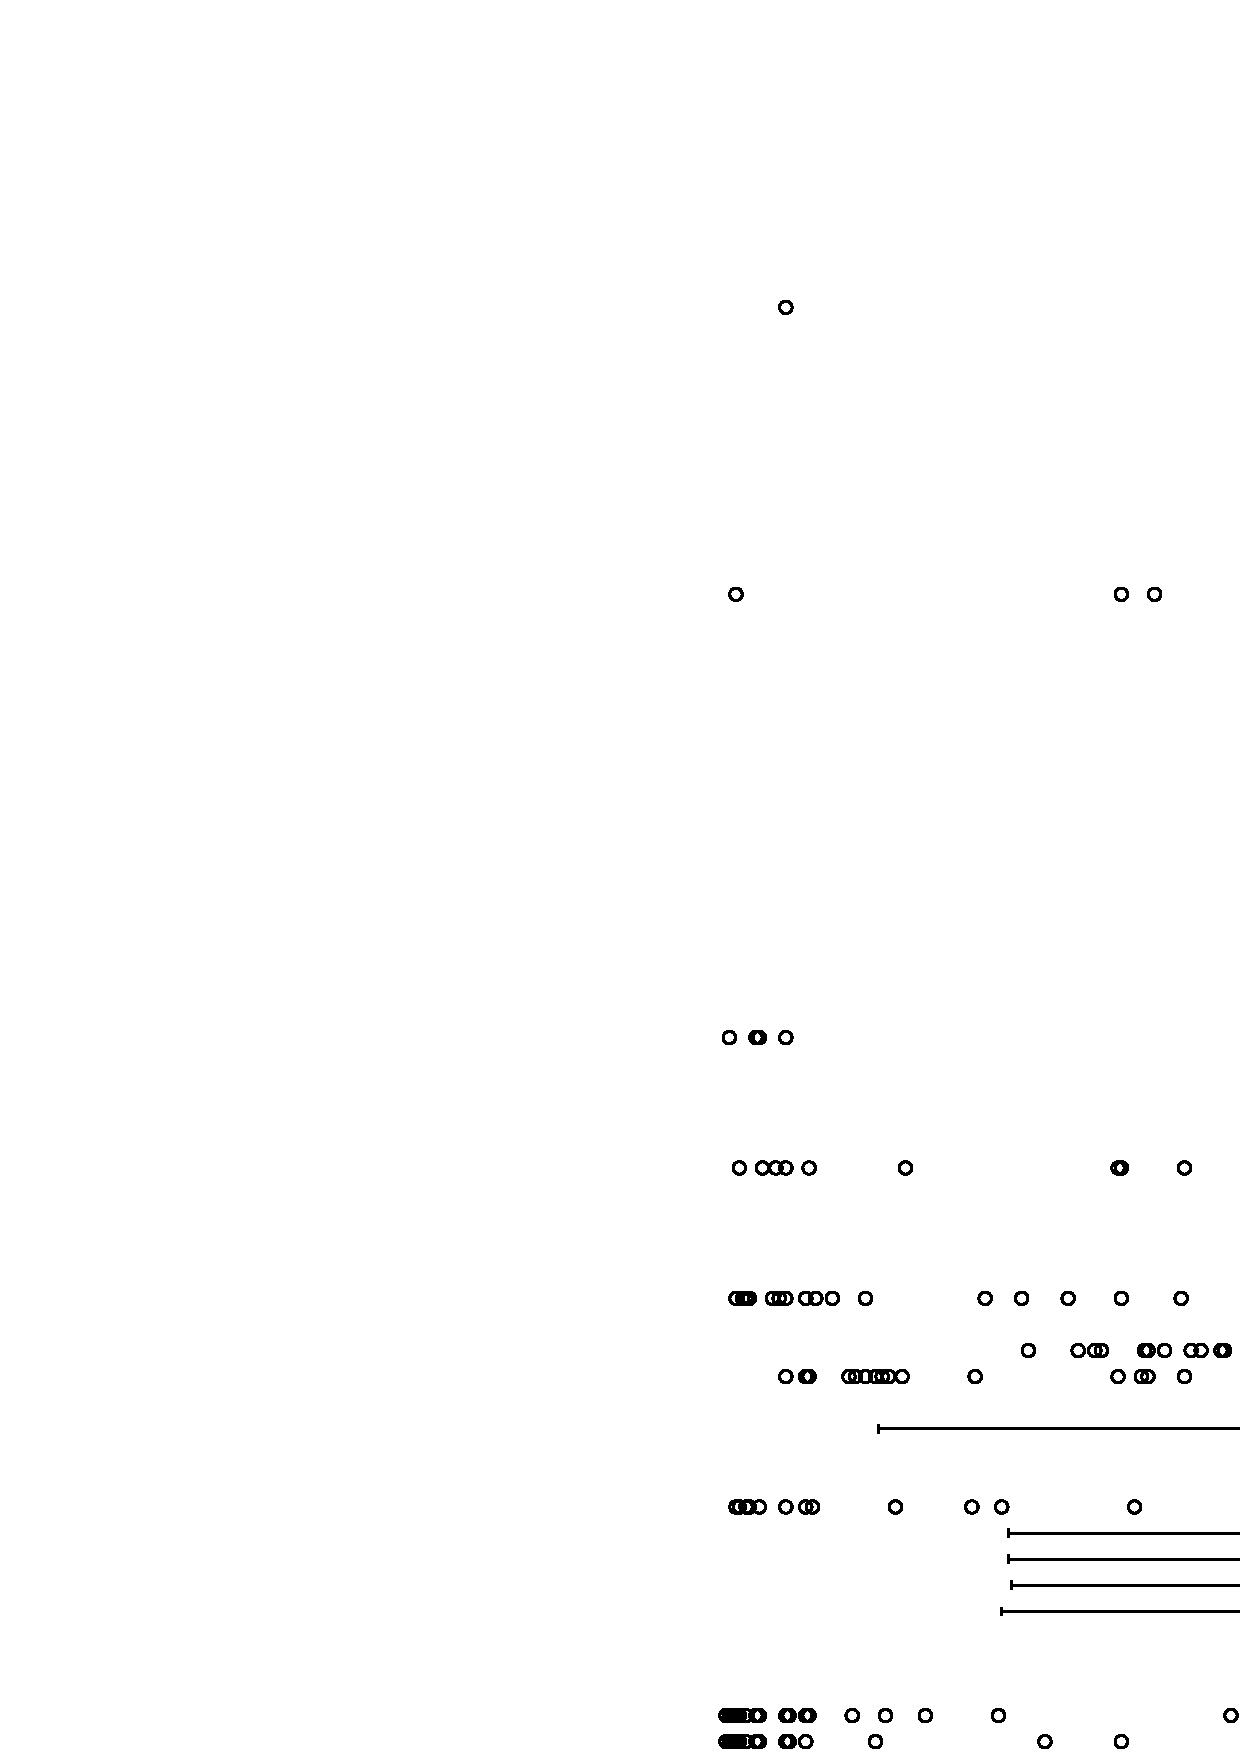
\includegraphics[width=\textwidth]{./boxplot_12_resist.pdf}
    \caption{The fixation probabilities \(x_{N-1}\) for \(N=12\)}
\end{figure}

\begin{figure}[!hbtp]
    \centering
    \includegraphics[width=\textwidth]{./boxplot_13_resist.pdf}
    \caption{The fixation probabilities \(x_{N-1}\) for \(N=13\)}
\end{figure}

\begin{figure}[!hbtp]
    \centering
    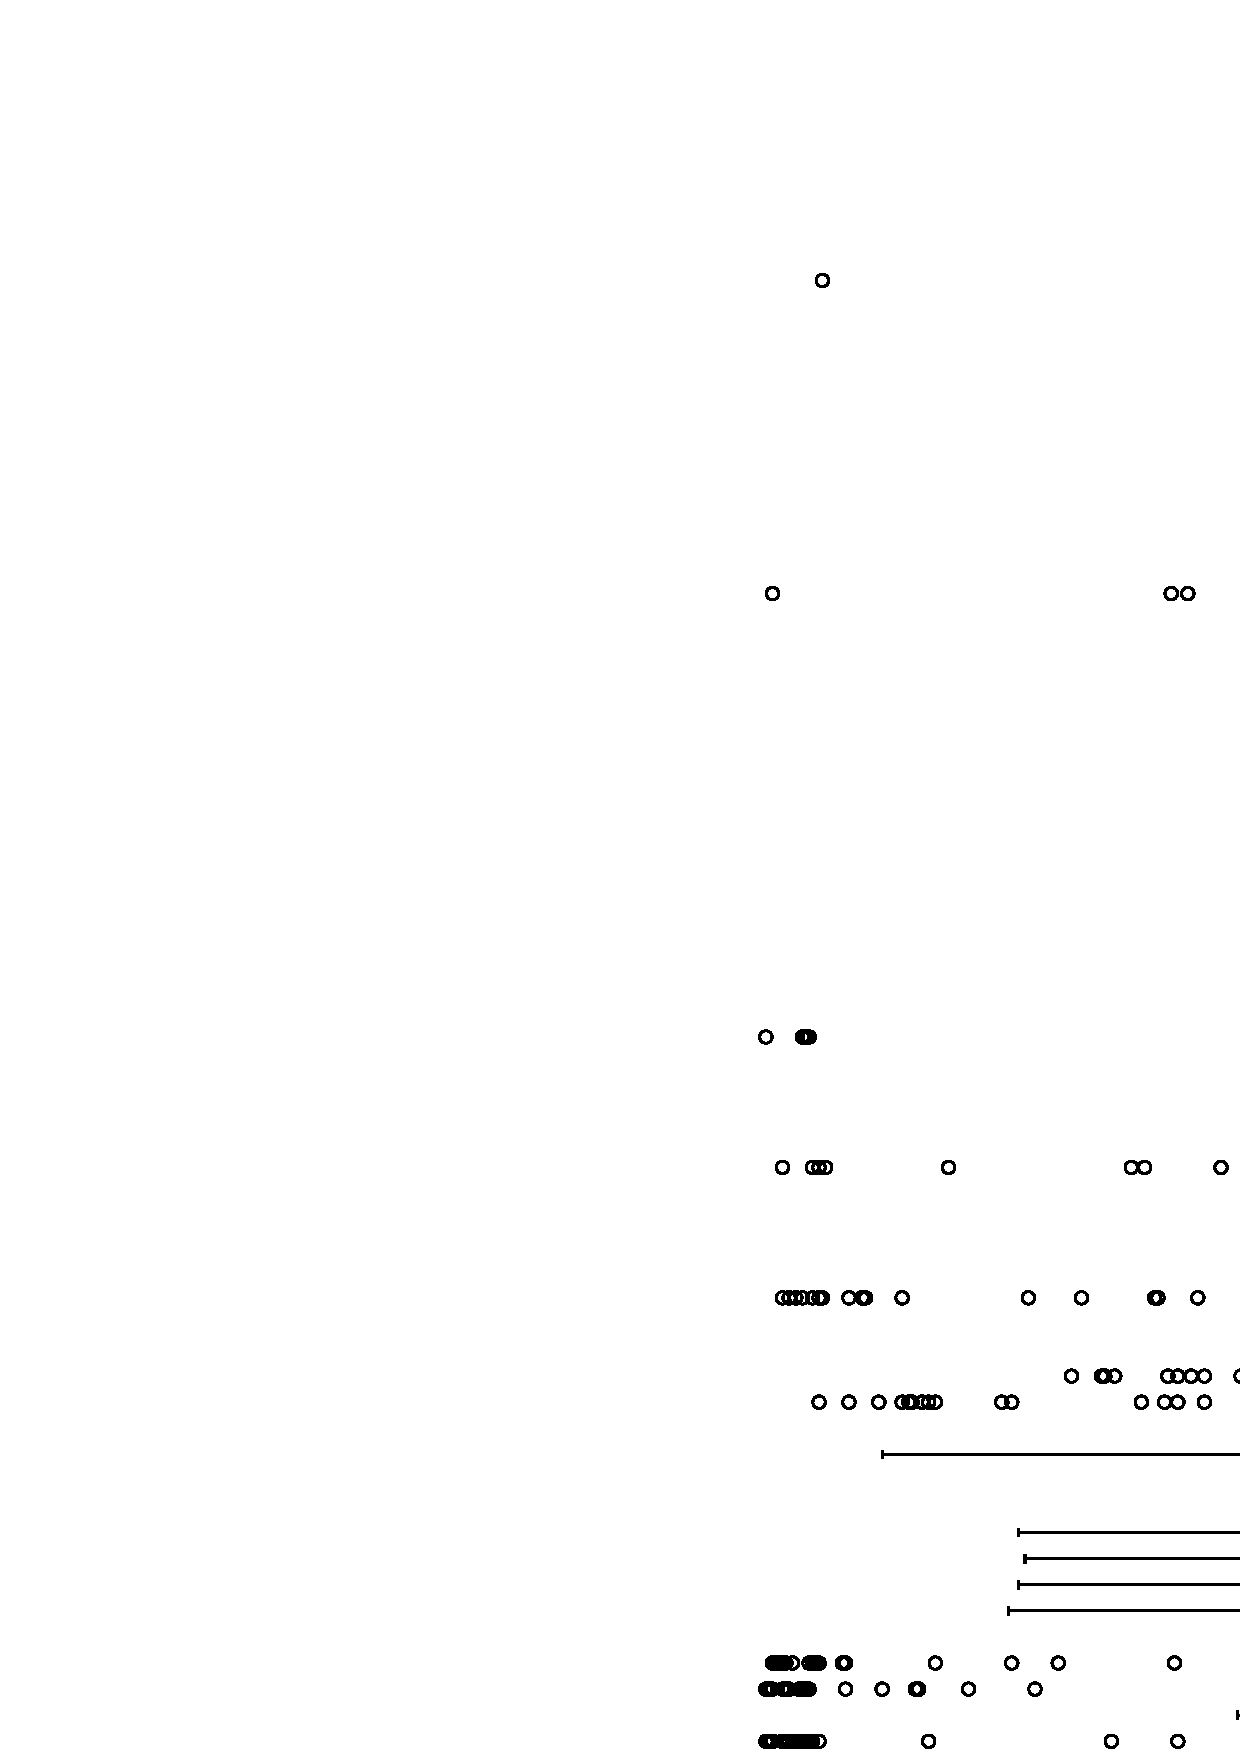
\includegraphics[width=\textwidth]{./boxplot_14_resist.pdf}
    \caption{The fixation probabilities \(x_{N-1}\) for \(N=14\)}
    \label{resistance-14}
\end{figure}

\end{document}

